%%%% IMPORTANT: to generate the nomenclature
%% makeindex main-survey-fnt.nlo -s nomencl.ist -o main-survey-fnt.nls


% !Mode:: "TeX:DE:UTF-8:Main"
%
%
%JOURNAL CODE  SEE DOCUMENTATION
\documentclass[biber]{nowfnt} % creates the journal version, needs biber version
%wrapper for book and ebook are created automatically.
\usepackage{imakeidx}
\usepackage[utf8]{inputenc}

%\usepackage{draftwatermark}
%\SetWatermarkLightness{0.95}

\def\withcolors{1}
\def\withnotes{0}
\usepackage{ccanonne}

\usetikzlibrary{shadows}
\usepackage{framed}
\usepackage{tabularx}
\usepackage[nocfg]{nomencl}
\makenomenclature

% Footnote without marker
\newcommand\extrafootertext[1]{%
    \bgroup
    \renewcommand\thefootnote{\fnsymbol{footnote}}%
    \renewcommand\thempfootnote{\fnsymbol{mpfootnote}}%
    \footnotetext[0]{#1}%
    \egroup
}

%%%%%%%%%%%%%%%%% Exercises %%%%%%%%%%%%%%%%%
\newtheorem{question}{Exercise}[chapter]

%\newcommand{\exinline}[1]{(\refstepcounter{question}Exercise~\thequestion\label{#1})}

\crefname{question}{Exercise}{Exercises}
\Crefname{question}{Exercise}{Exercises}
\crefname{claim}{Claim}{Claims}
%%%%%%%%%%%%%%%%%%%%%%%%%%%%%%%%%%%%%%%%%%%%


\newcolumntype{Y}{>{\centering\arraybackslash}X}
\renewcommand\tabularxcolumn[1]{m{#1}}% for vertical centering text in X column


\usepackage{physics} %% <- redefines var
\usepackage[fulladjust]{marginnote}
\renewcommand*{\marginfont}{\scriptsize}
\setlength{\marginparwidth}{15mm}
\newcommand{\exercise}[1]{\marginnote{\textbf{E:} #1}}

\ifnum\withnotes=1
\newcommand{\tbc}{\noindent\hl{\sc{}to be continued}\xspace}
\else
\newcommand{\tbc}{}
\fi


\newcommand{\nss}{\textcolor{red}{\ns_1}}
\newcommand{\nst}{\textcolor{red}{\ns_2}}
\newcommand{\nsu}{\textcolor{red}{\ns_3}}
\newcommand{\occur}{\textcolor{red}{N}}
\newcommand{\freq}{\textcolor{purple}{F}}


%% Subsections in the ToC (set to 1 for sections only)
\setcounter{tocdepth}{2}

%ARTICLE TITLE
\title{Topics and Techniques in Distribution Testing}


%ARTICLE SUB-TITLE
\subtitle{A Biased but Representative Sample}


%AUTHORS FOR COVER PAGE 
% separate authors by \and, item by \\
% Don't use verbatim or problematic symbols.
% _ in mail address should be entered as \_
% Pay attention to large mail-addresses ...

%if there are many author twocolumn mode can be activated.
%\booltrue{authortwocolumn} %SEE DOCUMENTATION
\maintitleauthorlist{
Cl\'ement L. Canonne \\
University of Sydney\\
clement.canonne@sydney.edu.au
}

%ISSUE DATA AS PROVIDED BY NOW
\issuesetup
{%
 copyrightowner={A.~Heezemans and M.~Casey},
 volume        = xx,
 issue         = xx,
 pubyear       = 2018,
 isbn          = xxx-x-xxxxx-xxx-x,
 eisbn         = xxx-x-xxxxx-xxx-x,
 doi           = 10.1561/XXXXXXXXX,
 firstpage     = 1, %Explain
 lastpage      = 18
 }

%BIBLIOGRAPHY FILE
\addbibresource{bibliography.bib}

% \usepackage{mwe}

%AUTHORS FOR ABSTRACT PAGE
\author[1]{Cl\'ement L. Canonne}

\affil[1]{University of Sydney; clement.canonne@sydney.edu.au}

\articledatabox{\nowfntstandardcitation}

\begin{document}
\makeabstracttitle
\begin{abstract}
We focus on some specific problems in distribution testing,
taking goodness-of-fit as a running example. In particular,
we do not aim to provide a comprehensive summary of all
the topics in the area; but will provide self-contained proofs and derivations of the main results, trying
to highlight the unifying techniques.
\end{abstract}

%%%%%%%%%%%%%%%%%%%%%%%%%%%%%%%%%%%%%%%%%%%%%%%%%%%%%%%%%%%%%%
%%%%%%%%%%%%%%%%%%%%%%%%%%%%%%%%%%%%%%%%%%%%%%%%%%%%%%%%%%%%%%
\nomenclature[1]{$a_n \lesssim b_n$}{There exists a constant $C>0$ such that $a_n\leq C\cdot b_n$ for every $n$. Similar to $a_n = O(b_n)$, but not necessarily asymptotic, and easier to write.}
\nomenclature[2]{$a_n \asymp b_n$}{Both $a_n \lesssim b_n$ and $b_n \lesssim a_n$. Similar to $a_n = \Theta(b_n)$, but not necessarily asymptotic, and easier to write.}
\nomenclature[3]{$a_n = O(b_n)$}{There exist a constant $C>0$ and a value $n_0$ such that $a_n\leq C\cdot b_n$ for every $n \geq n_0$.}
\nomenclature[4]{$a_n = \Omega(b_n)$}{There exist a constant $C>0$ and a value $n_0$ such that $a_n\geq C\cdot b_n$ for every $n \geq n_0$. This is equivalent to $b_n = O(a_n)$.}
\nomenclature[5]{$a_n = \Theta(b_n)$}{Both $a_n = \Omega(b_n)$ and $a_n = O(b_n)$.}
%\nomenclature{$x\sim \p$}{$x$ is sampled from the probability distribution $\p$}
\nomenclature[6]{$a_n {\displaystyle\operatorname*{\sim}_{n\to \infty}} b_n$}{Asymptotic equivalence: $\lim_{n\to\infty} \frac{a_n}{b_n} = 1$ (stronger than $a_n = \Theta(b_n)$, as the ``hidden constant'' is $1$).}
\nomenclature[7]{$a_n \gg b_n$}{(Informal) $a_n$ is much larger than, or ``sufficiently'' large compared to, $b_n$.}
\nomenclature[8]{$\log$, $\ln$}{Throughout, $\log$ denotes the logarithm in base 2 and $\ln$ the natural logarithm.}
\printnomenclature
%%%%%%%%%%%%%%%%%%%%%%%%%%%%%%%%%%%%%%%%%%%%%%%%%%%%%%%%%%%%%%
%%%%%%%%%%%%%%%%%%%%%%%%%%%%%%%%%%%%%%%%%%%%%%%%%%%%%%%%%%%%%%
\chapter{What is distribution testing?}
  \label{chap:what}
This survey serves as an introduction and detailed overview of some topics in (probability) distribution testing, an area of theoretical computer science which falls under the general umbrella of \emph{property testing}, and sits at the intersection of computational learning, statistical learning and hypothesis testing, information theory, and (depending whom one asks) the theory of machine learning. Broadly speaking, distribution testing is concerned with the following type of questions: 
\begin{framed}
 Given a \textbf{small} number of independent data points from some blackbox random source, can we \textbf{efficiently} decide whether the distribution of the data follows some purported model (``property''), or is statistically far from doing so?
\end{framed}

Of course, there are many details to be made precise here. What type of assumptions on the data do we make -- is it discrete, continuous, univariate, high-dimensional?  What do we mean by ``efficiently'' -- the number of data points (data efficiency), the running time of our algorithms (time efficiency), both? What do we mean by ``far'' -- what notion of distance are we considering? And what type of error do we allow -- false positives (Type I), false negative (Type II)?

Some of these are left flexible, as we will see below when formally introducing the setting of distribution testing. However, the general idea is to focus on \emph{finite sample guarantees} (no qualitative limiting statements as data size grows to infinity), for a \emph{fixed error probability target} $\errprob$ controlling both Type I and Type II, and making \emph{as few assumptions as possible} under the (composite) alternative hypothesis. That is, we will answer questions of the form ``either the distribution of the data satisfies the property, or it is \emph{pretty much anything} far from that.''


Adopting a Computer Science viewpoint, we will also assume that the ``size'' of the object considered -- typically, the domain size for discrete data -- is large, which allows us to focus on the first-order dependence on this quantity. This also implies we typically consider a \emph{worst-case} (minimax) setting with respect to this quantity, making statements about the worst-case data size, or time, required to achieve our goal. This does not means the algorithms and ideas obtained do not lead to ``practical'' algorithms: rather, that people working in distribution testing are quite pessimistic and paranoid in nature, and want the guarantee that things are \emph{never} too slow before the promise that they \emph{often} are quite fast. (Moreover, as we will see later, the worst-case instances for most of our testing tasks are actually quite natural, and likely to arise in practice! Paranoia, for once, may be warranted.)

\paragraph{A note.} For simplicity, throughout this survey we will sweep under the rug many measure-theoretic subtleties, and assume probability distributions, probability density functions (pdf), and probability mass functions (pmf) exist whenever required, and are suitably well-behaved. We will also typically identify a probability distribution with its pdf or pmf, and by a slight abuse of notation use $\p$ indifferently for the distribution itself and its pdf. Most, if not all, of those subtleties can be handled by inserting the words ``Radon--Nikodym,'' ``measurable,'' and ``counting measure'' in suitable places and order.

\section{Formulation, and relation to Hypothesis Testing}


In what follows, $\ab\in\N$ will be used to parametrize the domain of the probability distributions: namely, $\distribs{\ab}$ will denote the set of probability distributions over a (known) domain $\domain_\ab$.

We begin with the notion of distance we will be concerned about, the total variation distance (also known as \emph{statistical distance}):
\begin{definition}[Total variation distance]
  \label{def:tv}
  The \emph{total variation distance} between two probability distributions $\p,\q\in\distribs{\ab}$ is given by
  \[
    \totalvardist{\p}{\q} = \sup_{S\subseteq \domain_\ab} (\p(S)-\q(S))\,.
  \]
  Given a subset $\class\subseteq\distribs{\ab}$ of distributions, we further define the distance from $\p\in\distribs{\ab}$ to $\class$ as $\totalvardist{\p}{\class} \eqdef \inf_{\q\in\class} \totalvardist{\p}{\q}$, and will say that $\p$ is \emph{$\dst$-far from $\class$} if $\totalvardist{\p}{\class} > \dst$.
\end{definition}
One can check that $\dtv$ defines a metric on $\distribs{\ab}$, and takes values in $[0,1]$.\exercise{Check it!} Moreover, the total variation distance exhibits several important properties, some of which will be detailed at length in~\cref{app:distances}; we recall a crucial one below.

\begin{fact}[Data Processing Inequality]
  \label{fact:dpi}
  Suppose $X$ and $Y$ are independent random variables with distributions $\p$ and $\q$, and let $f$ be any (possibly randomized) function independent of $X,Y$. Then the probability distributions $\p_f$ and $\q_f$ of $f(X)$ and $f(Y)$ satisfy
  \[
      \totalvardist{\p_f}{\q_f} \leq \totalvardist{\p}{\q}\,.
  \]
  That is, \emph{postprocessing cannot increase the total variation distance.}
\end{fact}


Assuming that $\p,\q$ are absolutely continuous with respect to some dominating measure $\mu$,
  \begin{equation}
    \totalvardist{\p}{\q} = \frac{1}{2}\int \abs{\dv{\p}{\mu}-\dv{\q}{\mu}}\dd{\mu}
  \end{equation}
  In the discrete case where $\p,\q$ are both over $\N$ or a finite domain, this leads to
  \begin{equation}
    \label{eq:tv:l1}
    \totalvardist{\p}{\q} = \frac{1}{2}\normone{\p-\q}
  \end{equation}
  that is, ``total variation is half the $\lp[1]$ distance between pmfs.'' This turns out to be a very useful connection, since $\lp[p]$ norms are quite well-studied beasts: we get to use our arsenal of geometric inequalities --- H\"older, Cauchy--Schwarz, and monotonicity of $\lp[p]$ norms, to name a few.\smallskip

%nondecreasing in their first argument and nonincreasing in the last two
One last piece of terminology: a \emph{property}\index{property} of distributions is a predicate we are interested in (\eg ``is the probability distribution unimodal?''). By identifying the predicate with the set of objects which satisfy it, we can equivalently view a property of distributions as a \emph{subset} of probability distributions (typically, with some interesting structure). Which is what we will do: throughout, a property is just an arbitrary subset of distributions we are interested in. With this in hand, we are ready to provide a formal definition of what a ``testing algorithm'' is.
\begin{definition}[Testing algorithm]
  \label{def:testing}
Let $\property= \bigcup_{\ab=1}^\infty \property_\ab$ and $\class= \bigcup_{\ab=1}^\infty \class_\ab$ be two properties of probability distributions, where $\property_\ab, \class_\ab\subseteq \distribs{\ab}$ for all $\ab$; and $\ns\colon\N\times(0,1]\times(0,1]\to\N$, $\tc\colon\N\times(0,1]\times(0,1]\to\N$ be two functions. A \emph{testing algorithm for \property under $\class$ with sample complexity $\ns$ and time complexity $\tc$} is a (possibly randomized) algorithm $\Algo$ which, on input $\ab\in\N,\dst \in(0,1], \errprob\in(0,1]$, and a multiset $S$ of $\ns(\ab,\dst,\errprob)$ elements of $\domain_\ab$, runs in time at most $\tc(\ab,\dst,\errprob)$ and outputs $\mathbf{b} \in\{\reject,\accept\}$ such that the following holds.
\begin{itemize}
  \item If $S$ is \iid from some $\p\in\property_\ab$, then $\probaDistrOf{S,\Algo}{\mathbf{b}=\accept} \geq 1-\errprob$;
  \item If $S$ is \iid from some $\p\in\class_\ab$ such that $\totalvardist{\p}{\property_\ab} > \dst$, then $\probaDistrOf{S,\Algo}{\mathbf{b}=\reject} \geq 1-\errprob$,
\end{itemize}
where in both cases the probability is over the draw of the \iid sample $S$ from the (unknown) $\p$, and the internal randomness of $\Algo$.
\end{definition}
\noindent The \emph{sample complexity of testing \property under $\class$} is then the minimum sample complexity $\ns(\ab,\dst,\errprob)$ achievable by a testing algorithm.\smallskip

%%%%%%%%%%%%%%%%%%%%%%%%%%%%%%%%%%%%%%%%%%%%%%%%%%%%%%%%%%%%%%%%%%%%%%%%%%%%%%%%
\begin{figure}[htbp]\centering

\tikzset {_3eubqr20l/.code = {\pgfsetadditionalshadetransform{ \pgftransformshift{\pgfpoint{0 bp } { 0 bp }  }  \pgftransformrotate{0 }  \pgftransformscale{2.64 }  }}}
\pgfdeclarehorizontalshading{_y5uoy9rpz}{150bp}{rgb(0bp)=(0.99,0.97,0.93);
rgb(54.285714285714285bp)=(0.99,0.97,0.93);
rgb(61.96428571428571bp)=(0.98,0.95,0.95);
rgb(100bp)=(0.98,0.95,0.95)}
\tikzset{every picture/.style={line width=0.75pt}} %set default line width to 0.75pt        

\begin{tikzpicture}[x=0.75pt,y=0.75pt,yscale=-1.3,xscale=1.3]
%uncomment if require: \path (0,300); %set diagram left start at 0, and has height of 300

%Shape: Polygon Curved [id:ds24835565753561872] 
\draw  [draw opacity=0.05][shading=_y5uoy9rpz,_3eubqr20l] (228.87,88.88) .. controls (266.87,64.88) and (266.87,111.88) .. (282.87,123.88) .. controls (298.87,135.88) and (360.87,96.88) .. (335.87,141.88) .. controls (310.87,186.88) and (389.87,249.88) .. (305.87,226.88) .. controls (221.87,203.88) and (251.87,247.88) .. (208.87,236.88) .. controls (165.87,225.88) and (201.87,193.88) .. (183.87,172.88) .. controls (165.87,151.88) and (157.87,118.88) .. (191.87,123.88) .. controls (225.87,128.88) and (190.87,112.88) .. (228.87,88.88) -- cycle ;
%Shape: Circle [id:dp2977666721327956] 
\draw  [draw opacity=0][fill={rgb, 255:red, 253; green, 170; blue, 30 }  ,fill opacity=0.70 ][general shadow={fill={rgb, 255:red, 245; green, 166; blue, 35 },shadow xshift=0pt,shadow yshift=0pt, opacity=0 }] (242,165.5) .. controls (248,147) and (253,132) .. (271.5,132) .. controls (290,132) and (305,147) .. (308,165.5) .. controls (310,184) and (290,199) .. (271.5,199) .. controls (253,199) and (238,184) .. (242,165.5) -- cycle ;
%Shape: Circle [id:dp2977666721327956] 
\draw  [draw opacity=0.05, scale=0.8,xshift=51pt,yshift=31pt][fill={rgb, 255:red, 253; green, 170; blue, 30 }  ,fill opacity=0.99 ][general shadow={fill={rgb, 255:red, 245; green, 166; blue, 35 },shadow xshift=0pt,shadow yshift=0pt, opacity=0 }] (242,165.5) .. controls (248,147) and (253,132) .. (271.5,132) .. controls (290,132) and (305,147) .. (308,165.5) .. controls (310,184) and (290,199) .. (271.5,199) .. controls (253,199) and (238,184) .. (242,165.5) -- cycle ;
%Shape: Ellipse [id:dp5805520465941827] 
%\draw  [draw opacity=0][fill={rgb, 255:red, 233; green, 152; blue, 19 }  ,fill opacity=1 ] (265.43,186.22) .. controls (261.59,181.1) and (265.3,171.81) .. (273.73,165.48) .. controls (282.16,159.14) and (292.12,158.15) .. (295.97,163.27) .. controls (299.81,168.39) and (296.1,177.67) .. (287.67,184.01) .. controls (279.23,190.35) and (269.28,191.34) .. (265.43,186.22) -- cycle ;
%Shape: Block Arc [id:dp4643699266244976] 
%\draw  [draw opacity=0.0][fill={rgb, 255:red, 255; green, 255; blue, 255 }  ,fill opacity=1 ] (181.64,151.16) .. controls (181.68,147.43) and (182.42,143.85) .. (183.93,140.65) .. controls (186.88,134.44) and (192.19,130.86) .. (198.43,130.09) -- (201.36,139.03) .. controls (196.68,139.19) and (192.72,141.5) .. (190.65,145.86) .. controls (189.57,148.15) and (189.12,150.76) .. (189.23,153.51) -- cycle ;
%Shape: Block Arc [id:dp28641962733560566] 
%\draw  [draw opacity=0.0][fill={rgb, 255:red, 255; green, 255; blue, 255 }  ,fill opacity=1 ] (209.55,189.06) .. controls (207.11,187.92) and (204.68,186.55) .. (202.32,184.94) .. controls (197.19,181.46) and (192.99,177.29) .. (189.87,172.88) -- (197.79,170.62) .. controls (200.18,173.44) and (203.18,176.15) .. (206.68,178.53) .. controls (208.26,179.61) and (209.87,180.57) .. (211.49,181.4) -- cycle ;
\node at (160,100) (nodeclass) {$\distribs{\ab}$};
\node at (240,120) (nodeclass) {$\class_\ab$};
\node at (245,175) (nodeclass) {\scriptsize$\dst$};
\node at (275,165) (nodeproperty) {$\property_\ab$};
\end{tikzpicture}
\caption[An example of property to test. Here, $\property_\ab\subseteq \class_\ab\subseteq \distribs{\ab}$, where the property $\property_\ab$ is depicted as the inner orange area (``yolk''), and the ``egg white'' is the  area of rejection, \ie the subset of $\class_\ab$ at total variation distance at least $\dst$ from $\property_\ab$.]{An example of property to test. Here, $\property_\ab\subseteq \class_\ab\subseteq \distribs{\ab}$, where the property $\property_\ab$ is depicted as the inner orange area (``yolk''), and the ``egg white'' is the  area of rejection, \ie the subset of $\class_\ab$ at total variation distance at least $\dst$ from $\property_\ab$.\label{fig:propertytesting}\footnotemark}
\end{figure}

%%%%%%%%%%%%%%%%%%%%%%%%%%%%%%%%%%%%%%%%%%%%%%%%%%%%%%%%%%%%%%%%%%%%%%%%%%%%%%%%%%%%%%%%%%%%%%%%%%%%%%%%%%%%%%%%%%%%%%%%%%%%%%%%%%%%%%%%%%%%%%%%%%%%%%%%%%%%%%%%
%% Adapted from https://tex.stackexchange.com/questions/74168/how-can-i-draw-an-egg-using-tikz/598086#598086
%%%%%%%%%%%%%%%%%%%%%%%%%%%%%%%%%%%%%%%%%%%%%%%%%%%%%%%%%%%%%%%%%%%%%%%%%%%%%%%%%%%%%%%%%%%%%%%%%%%%%%%%%%%%%%%%%%%%%%%%%%%%%%%%%%%%%%%%%%%%%%%%%%%%%%%%%%%%%%%%

A few remarks are in order. First, in most of our applications we will take $\class_\ab=\distribs{\ab}$, so that the unknown distribution $\p$ is \emph{a priori} arbitrary, and the goal is to check whether it belongs to the subset (property) of interest $\property_\ab$. However, this need not always be the case, and we may want to choose $\class_\ab$ differently to perform hypothesis testing \emph{under structural assumptions}: for instance, to test whether an unknown unimodal distribution is actually Binomial (in this case, $\property_\ab \subsetneq \class_\ab\subsetneq \distribs{\ab}$), or if say a log-concave distribution is monotone (in which case there is no inclusion relation between $\property_\ab$ and $\class_\ab$, and both are strict subsets of $\distribs{\ab}$).

Another important point is that, while our main focus will be on \emph{discrete} distributions,~\cref{def:testing} allows for continuous distributions as well. Finally, the above definition is quite flexible, and can be seen to allow for testing \emph{multiple} distributions: for instance, taking $\domain_\ab=[\ab]\times[\ab]$, $\class_\ab \eqdef \setOfSuchThat{ \p\in\distribs{\ab} }{ \p=\p_1\otimes\p_2 }$ (product distributions), and $\property_\ab \eqdef \setOfSuchThat{\p_1\otimes\p_2 \in \class_\ab}{\p_1=\p_2}$, we obtain the question of two-sample testing (a.k.a.\ closeness testing), which asks to test whether two unknown distributions over $[\ab]$ are equal, or far from each other.
%%%%%%%%%%%%
\footnotetext{TikZ code for \cref{fig:propertytesting} adapted from~\url{https://tex.stackexchange.com/a/598086/31516}.}
%%%%%%%%%%%%
\paragraph{Dependence on the error probability $\errprob$.} Our definition of testing algorithm leaves the error probability $\errprob$ as a free parameter; however, it is quite common in the distribution testing literature to set it as some arbitrary constant smaller than $1/2$ (usually $1/3$). Indeed, by a standard argument,\index{probability amplification} an error probability $1/3$ can be driven down to arbitrary $\errprob$ at the price of a $\bigO{\log(1/\errprob)}$ factor in the sample complexity. 
\begin{lemma}[Error probability amplification]
  \label{lemma:error:proba:amplification}
  Fix $\property$ and $\class$, and suppose there exists a testing algorithm $\Algo$ for $\property$ under $\class$ with sample complexity $\ns(\ab,\dst,1/3)$ and time complexity $\tc(\ab,\dst,1/3)$. Then there is a testing algorithm $\Algo'$ for $\property$ under $\class$ with sample and time complexities $\ns'(\ab,\dst,\errprob) \eqdef \ns(\ab,\dst,1/3)\clg{18\ln(1/\errprob)}$ and $\tc'(\ab,\dst,\errprob) \eqdef \bigO{ \tc(\ab,\dst,1/3) \log(1/\errprob)}$.\cmargin{Logarithm is binary!}
\end{lemma}
\begin{proof}[Proof sketch]
Fix $\property$, $\class$, $\Algo$ as in the statement. Given $\ab,\dst$, and $\errprob\in(0,1]$, let $\Algo'$ be the algorithm which takes as input a multiset of $\ns'(\ab,\dst,\errprob)$ elements, partitions it (arbitrarily) in $m \eqdef \clg{18\ln(1/\errprob)}$ disjoint multisets $S_1,\dots, S_m$, runs $\Algo$ independently on those $m$ multisets with error probability $1/3$ to get $\mathbf{b}_1,\dots,\mathbf{b}_m$, and finally outputs the majority answer $\mathbf{b} \eqdef \indic{\sum_{i=1}^m \mathbf{b}_i \geq m/2}$. The running time is dominated by the $m$ executions, giving the claimed $\bigO{m\cdot \tc(\ab,\dst,1/3)}$ bound. Thus, it suffices to check that the output is correct with probability at least $1-\errprob$; this in turn follows from a Hoeffding bound (\cref{theo:hoeffding}). Indeed, by assumption, each $\mathbf{b}_i$ is independently correct with some probability $p\geq 2/3$. Letting $X_i \sim \bernoulli{p}$ be the indicator of the event ``{$\mathbf{b}_i$ is the correct output},'' we have
\[
  \probaOf{\mathbf{b} \text{ incorrect}} = \probaOf{ \frac{1}{m}\sum_{i=1}^m X_i  < \frac{1}{2} } \leq e^{-2(p-1/2)^2m} \leq e^{-m/18} \leq \errprob\,,
\]
where we used our setting of $m$ in the last inequality. 
\end{proof}
Importantly, this logarithmic dependence is not always the right one: as we will see in~\cref{chap:identity}, there exist natural problems for which the right dependence on the error probability only scales as $\sqrt{\log(1/\errprob)}$.

\paragraph{The learning baseline.}
Before setting out to design specific algorithms for various testing tasks and analyze their performance, it is good to have some sort of baseline to compare the result to. The most natural one is the \emph{testing-by-learning} approach, which can essentially be summarized as follows: the sample complexity of testing $\property= \bigcup_{\ab=1}^\infty \property_\ab$ under $\class= \bigcup_{\ab=1}^\infty \class_\ab$ is at most the sample complexity of, given $\ab$, \emph{learning} an arbitrary distribution from $\property_\ab\cup\class_\ab$. More specifically, we have the following:
\begin{lemma}[Testing by Learning]
  Fix any $\property= \bigcup_{\ab=1}^\infty \property_\ab$ and $\class= \bigcup_{\ab=1}^\infty \class_\ab$, and let $\ns_{\mathcal{L}}(\ab,\dst,\errprob)$ denote the sample complexity of learning an arbitrary probability distribution from $\property_\ab\cup\class_\ab\subseteq \distribs{\ab}$ to total variation $\dst$ with error probability at most $\errprob$. Then, the sample complexity $\ns$ of testing \property under $\class$ satisfies
  \[
      \ns(\ab,\dst,\errprob) \leq \ns_{\mathcal{L}}(\ab,\tfrac{\dst}{2},\errprob)\,.
  \]
  This is not necessarily achieved by a computationally efficient tester.
\end{lemma}
\begin{proof}
Fix a learning algorithm $\Algo$ for $\property_\ab\cup\class_\ab$ with sample complexity $\ns\eqdef \ns_{\mathcal{L}}(\ab,\tfrac{\dst}{2},\errprob)$. By running it on $\ns$ \iid samples from $\p$ (which we are promised either belongs to $\property_\ab$ or $\class_\ab$), we obtain a distribution $\hat{\p}$ such that $\totalvardist{\hat{\p}}{\p} \leq \dst/2$ with probability at least $1-\delta$. Assuming this is the case, then (i)~if $\p\in\property_\ab$, then of course $\totalvardist{\hat{\p}}{\property} \leq \dst/2$; while (ii)~if $\totalvardist{\p}{\property} > \dst$, by the triangle inequality (since total variation distance is a metric) we must have $\totalvardist{\hat{\p}}{\property} > \dst/2$. 

But we have an explicit description of $\hat{\p}$ in our hands, so we can check which of the two cases holds -- this may not be computationally efficient, but does not require any additional sample from $\p$. Thus, we have a \emph{bona fide} testing algorithm for \property under $\class$.
\end{proof}
Importantly, this baseline is with respect to the sample complexity of learning distributions from $\property_\ab\cup\class_\ab$, \emph{not} just $\property_\ab$: the latter is in general much larger! For instance, if $\property_\ab$ is a singleton but $\class_\ab=\distribs{\ab}$ (\eg as in identity testing, which we shall see in~\cref{chap:identity}) then learning $\property_\ab$ has sample complexity $0$, but learning $\property_\ab\cup\class_\ab=\distribs{\ab}$ has sample complexity $\Omega(\ab)$. This leads us to our baseline: since $\property_\ab\cup\class_\ab\subseteq \distribs{\ab}$, the sample complexity of \emph{any} distribution testing problem is at most the sample complexity of learning an arbitrary distribution over a known domain of the same size, which we record below:
\begin{theorem}[Learning baseline]
  \label{theo:learningbaseline}
  The sample complexity of learning an arbitrary probability distribution from $\distribs{\ab}$ to total variation $\dst$ with error probability at most $\errprob$ is
  \[
      \ns_{\mathcal{L}}(\ab,\dst,\errprob) = \bigTheta{\frac{\ab+\log(1/\errprob)}{\dst^2}}\,,
  \]
  giving an upper bound on the sample complexity of any testing problem.
\end{theorem}
The proof can be found in various places; \eg~\citet{KOPS:15,Canonne20:learning:short}. This testing-by-learning baseline, which is linear in the domain size $\ab$, motivates the name commonly given to testing algorithms which achieve significantly better sample complexity: \emph{sublinear algorithms}.

%%%%%%%%%%%%%%%%%%%%%%%%%%%%%%%%%%%%%%%%%%%%%%%%%%%%%%%%
%%%%%%%%%%%%%%%%%%%%%%%%%%%%%%%%%%%%%%%%%%%%%%%%%%%%%%%%
\section{Why total variation distance?}

The standard formulation of distribution testing, as stated in~\cref{def:testing}, is tied to a specific metric between probability distribution: the total variation distance (\cref{def:tv}). It is natural to wonder of that choice is arbitrary, and, if not, what motivates it.
\begin{itemize}
  \item Total variation distance provides a \emph{very strong guarantee}, and for instance is the most stringent of all $\lp[p]$ norms. This has practical consequences: if a source of data passes the test, then it will by nearly ``as good as if it had the desired property'' as far as \emph{any} algorithm is concerned. 
  \item It is \emph{well-behaved}: total variation distance defines a proper metric, and thus satisfies for instance the triangle inequality (which cannot be said about, for instance, Kullback--Leibler divergence). It is also nicely bounded, and will not take infinite values due to pathological reasons.
  \item It satisfies the \emph{data processing inequality} (\cref{fact:dpi}), which means it is robust to preprocessing. If data comes from two sources close in total variation distance, then post-processing this data cannot make their distribution statistically further apart. This is not the case for, among others, the $\lp[2]$ metric.
  \item Its relation to hypothesis testing: total variation distance has a natural and precise interpretation in terms of \emph{distinguishability}. This is formalized in~\cref{lemma:pearsonneyman}, and makes total variation distance the ``right'' notion of distance in applications such as cryptography, and when arguing about indistinguishability of data sources.
  \item Its connection to other distance measures. Total variation distance enjoys various inequalities relating it to other distance measures such as Kullback--Leibler divergence, $\lp[p]$ metrics, Hellinger distance, Kolmogorov distance, and Wasserstein (Earthmover) metric. Some of those are elaborated upon in~\cref{app:distances}.
\end{itemize}

Of course, total variation distance also has its drawbacks: it is sometimes too stringent, especially when considering distributions over continuous domains: in that case, absent further assumptions on the unknown continuous density, the testing problem becomes trivially impossible~\citep{LeCam73}. It also does not ``tensorize'' well (as opposed to, say, Hellinger distance or Kullback--Leibler divergence), meaning that the total variation distance between product measures does not have a nice form with respect to the total variation distances between individual marginals. And indeed, there are pros and cons to each choice; although in this case the above should convince you that the pros vastly outnumber the cons.

\paragraph{Relation to hypothesis testing.} As aforementioned, there is a natural connection between total variation distance and hypothesis testing, which we recall below. 
\begin{lemma}[Pearson--Neyman]
  \label{lemma:pearsonneyman}
  Any (possibly randomized) statistical test which distinguishes between $\p_0$ and $\p_1$ from a single sample must have Type~I (false positive) and Type-II (false negative) errors satisfying
  \[
      \text{Type~I} + \text{Type~II} \geq 1- \totalvardist{\p_0}{\p_1}
  \]
  Moreover, this is achieved by the test which outputs $1$ if, and only if, the sample belongs to the set $S^\ast \eqdef \setOfSuchThat{x}{\p_1(x) > \p_0(x)}$.
\end{lemma}
\begin{proof}
Fix any test $\Algo$ distinguishing between two distributions $\p_0$ and $\p_1$, given a single observation. Letting $\alpha$ and $\beta$ denote the Type~I and Type-II errors of $\Algo$, we have
\begin{align*}
  \alpha+\beta 
  &= \probaDistrOf{\p_0,R}{\Algo(X,R)=1} + \probaDistrOf{\p_1,R}{\Algo(X,R)=0} \\
  &= \shortexpect_{R}[ \probaDistrOf{\p_0}{\Algo(X,R)=1} ] + \shortexpect_{\Algo}[ \probaDistrOf{\p_1}{\Algo(X,R)=0} ] \\
  &= \shortexpect_{R}[ \probaDistrOf{\p_0}{\Algo(X,R)=1} + \probaDistrOf{\p_1}{\Algo(X,R)=0} ]
%   \totalvardist{\p}{\q}
\end{align*}
where we denote by $R$ the internal randomness of $\Algo$. Since, for any fixed realization $r$ of this randomness $R$, the resulting test $\Algo(\cdot,r)$ is deterministic, we can define for any $r$ the \emph{acceptance region} $S_{\Algo,r} \eqdef \setOfSuchThat{x}{\Algo(x,r)=1}$, and write
\begin{align*}
  \alpha+\beta 
  &= \shortexpect_{R}[ \probaDistrOf{\p_0}{X \in S_{\Algo,R}} + \probaDistrOf{\p_1}{X \notin S_{\Algo,R}} ] \\
  &= 1+\shortexpect_{R}[ \p_0(S_{\Algo,R}) - \p_1(S_{\Algo,R}) ] \\
  &\geq 1 + \inf_{S}(\p_0(S) - \p_1(S)) \\
  &= 1 - \sup_{S}(\p_1(S) - \p_0(S)) \\
  &= 1- \totalvardist{\p_0}{\p_1}\,,
\end{align*}
as claimed. Finally, it is immediate from the definition of total variation distance that the proposed test satisfies $\text{Type~I} + \text{Type~II} = 1 + \p_0(S^\ast) - \p_1(S^\ast) = 1- \totalvardist{\p_0}{\p_1}$.
\end{proof}
%%%%%%%%%%%%%%%%%%%%%%%%%%%%%%%%%%%%%%%%%%%%%%%%%%%%%%%%
%%%%%%%%%%%%%%%%%%%%%%%%%%%%%%%%%%%%%%%%%%%%%%%%%%%%%%%%
\section{The road not taken: tolerant testing}
In~\cref{def:testing} and throughout this survey, we focus on the standard formulation version of testing, where the unknown distribution $\p$ either \emph{belongs} to the property $\cP_\ab$ or is far from it. A natural generalization of this, allowing for some ``tolerance'' to noise or misspecification in the former case, would be to ask to distinguish $\p$ \emph{close} to $\cP_\ab$ from $\p$ far from it. This is called \emph{tolerant testing}~\cite{ParnasRR06}, and is formalized by introducing two parameters $0\leq \dst' < \dst \leq 1$, and relaxing the first item of~\cref{def:testing} to 
\begin{quote}
If $S$ is \iid from some $\p\in\distribs{\ab}$ such that $\totalvardist{\p}{\property_\ab} \leq \dst'$, then $\probaDistrOf{S,\Algo}{\mathbf{b}=\accept} \geq 1-\errprob$;
\end{quote}
(Note then that our regular, ``non-tolerant'' testing corresponds to taking $\dst'=0$.) The tolerant testing task, sometimes called in Statistics testing with an \emph{imprecise null}, typically requires a much higher sample complexity than the non-tolerant one~\citep{VV:11:stoc}, and both algorithms and lower bounds are obtained via significantly different techniques. For this reason, we will not here discuss tolerant testing in much, or indeed any detail: the interested reader is referred to, \eg~\citet{WuY20} for a primer on some of those techniques, and to~\citet{CanonneJKL21} and references within for an overview of results on tolerant goodness-of-fit testing.
%%%%%%%%%%%%%%%%%%%%%%%%%%%%%%%%%%%%%%%%%%%%%%%%%%%%%%%%
%%%%%%%%%%%%%%%%%%%%%%%%%%%%%%%%%%%%%%%%%%%%%%%%%%%%%%%%
\section{Historical notes}
Hypothesis testing has a long and rich history in Statistics, starting with the work of~\citet{Pearson1900} introducing the $\chi^2$ test, and leading to substantial advances over the next century. While it is difficult and slightly dangerous to reduce twelve decades of intense research and study in a few sentences,\footnote{Which is exactly what the following paragraph will set out to do regardless.} standard approaches in Statistics share a few common features. First, they are \emph{asymptotic} in nature (as opposite to focusing on finite-sample guarantees), establishing and studying the limiting distribution of a given test as the sample size goes to infinity. This enables one to compute confidence intervals, and obtain a swath of information from the limiting distribution; but by itself provides little insight regarding the intermediate, finite-sample regime. Second, they tend to focus on the so-called Type~I error (significance of the test), \ie the probability to mistakenly reject the null hypothesis $\mathcal{H}_0$, and only after fixing this significance level set out to minimize the Type~II error (that is, maximize the \emph{power} of the test), which is the probability to mistakenly accept the alternative hypothesis $\mathcal{H}_1$. This is, again, an oversimplification; the reader should refer to, \eg~\citet{BalakrishnanW18} for a complementary and more detailed view. Nonetheless, these features are two of the most salient points of contrast with the very recent and related take on hypothesis testing from the theoretical computer science community, \emph{distribution testing}, which perhaps shares most similarity with the work of Ingster~\citep{Ingster86,Ingster97}.

Distribution testing was first introduced in an influential paper by~\citet{GoldreichGR98}, which formally defined the broader field of property testing; \citet{GoldreichR00} then specifically considered the question of testing uniformity of an unknown probability distribution (in an~$\lp[2]$ sense), using the collision-based tester to test whether a random walk had (approximately) reached its stationary distribution.

This was, however, only implicitly using uniformity testing as a subroutine in the context of testing some property (expansion) of bounded-degree graphs. The work of \citet{BatuFRSW00} first considers distribution testing for its own sake, studying the question of \emph{closeness testing} (\ie two-sample testing), where one seeks to decide from samples if two unknown distributions are equal. This initiated a long line of work on testing many properties~--~including uniformity, identity, closeness, monotonicity, independence (being a product distribution), to name only a few.

While the early papers focused on the dependence on the domain size $\ab$, treating the distance parameter $\dst$ as a small constant or a second-order concern, later works, beginning with~\citet{ChanDVV14}, started looking for the tight dependence on $\dst$ as well. Even more recently, the ``right'' dependence on $\errprob$, the error probability, has come into focus as well~\citep{DiakonikolasGPP18,DiakonikolasGKP21}. This, in some sense, brings the theoretical computer science closer to the information theory literature, where the focus on the \emph{error exponent} (that is, the rate at which the error probability decays exponentially, as a function of the other parameters) is the standard view.\cmargin{[citation needed]}

Another recent trend in distribution testing has been to consider different ``accesses'' to the data, rather than \iid samples: for instance, access to so-called conditional samples~\citep{CRS:15,CFGM:13}, or the ability to ask for, or observe, the probability of individual elements of the domain~\citep{RubinfeldS09,CanonneR14,OnakS18}. These types of access allow for much more efficient testing algorithms, but require significantly different algorithmic tools and proof techniques, and we will not discuss them here. For more on this, we defer the interested reader to another survey,~\citet{Canonne:15:Survey}.

Finally, over the past few years distribution testing has ventured into adjacent areas of computer science and information theory, by incorporating various constraints and resources into its formulation. Examples include data privacy (and, more specifically, \emph{differential privacy}~\citep{DworkMNS06} and its variants)~--~see, \eg \citep{KamathU20}, memory constraints, and bandwidth constraints~\citep{Tsitsiklis:93}; of which we will cover a fraction in~\cref{chap:constrained}. This has been done by borrowing, extending, and (re)discovering ideas and techniques from these areas and Statistics; somewhat satisfyingly, leading distribution testing back to some of its roots. 

This survey aims to describe some of these connections, and provide an overview of these ideas and techniques which took years for the author to learn about.



%%%%%%%%%%%%%%%%%%%%%%%%%%%%%%%%%%%%%%%%%%%%%%%%%%%%%%%%%%%%%%
%%%%%%%%%%%%%%%%%%%%%%%%%%%%%%%%%%%%%%%%%%%%%%%%%%%%%%%%%%%%%%
\chapter{Testing goodness-of-fit of univariate distributions}
  \label{chap:identity}
%%%%%%%%%%%%%%%%%%%%%%%%%%%%%%%%%%%%%%%%%%%%%%%%%%%%%%%%%%%%%%%%%%%%%%%%%
%%%%%%%%%%%%%%%%%%%%%%%%%%%%%%%%%%%%%%%%%%%%%%%%%%%%%%%%%%%%%%%%%%%%%%%%%
\section{Uniformity testing}
\cnote{Thorough presentation of the many algorithms for uniformity testing,
with proofs, and relative advantages of each.}

It is known~\citep{Paninski08} that the sample complexity of uniformity testing with distance parameter $\dst\in(0,1]$ is $\Theta(\sqrt{\ab}/\dst^2)$. That's nice. Now, \emph{how do we perform uniformity testing, though?} 
There are several things to consider in a testing algorithm. For instance:
\begin{description}
  \item[Data efficiency:] does the algorithm achieve the optimal sample complexity $\Theta(\sqrt{\ab}/\dst^2)$?
  \item[Time efficiency:] how fast is the algorithm to run (as a function of $\ab,\dst$, and the number of samples $\ns$)?
  \item[Memory efficiency:] how much memory does the algorithm require (as a function of $\ab,\dst$, and $\ns$)?
  \item[Simplicity:] is the algorithm simple to describe and implement?
  \item[``Simplicity'':] is the algorithm simple to \emph{analyze}?
  \item[Robustness:] how \emph{tolerant} is the algorithm to breaches of the promise? That is, does it accept distributions which are not \emph{exactly} uniform as well, or is it very brittle?
  \item[Elegance:] That's, like, your opinion, man.
  \item[Generalizable:] Does the algorithm have other features that might be desirable in other settings?
\end{description}

\cref{tab:summary:uniformity:testing} summarizes a few of those criteria.
\begin{table}[ht]\centering\footnotesize
  \def\arraystretch{1.25}%  1 is the default, change whatever you need
% %   \begin{adjustwidth}{0in}{0in}% adjust the L and R margins by 1 inch
  \begin{tabularx}{\textwidth}{|Y|Y|Y|Y|}
  \hline
     & \bf Sample complexity & \bf Notes & \bf References \\\hline
    \bf Collision-based & $\dfrac{\ab^{1/2}}{\dst^2}$ & Tricky & \cite{GoldreichR00,DiakonikolasGPP19} \\\hline
    \bf Unique elements & $\dfrac{\ab^{1/2}}{\dst^2}$ & $\dst \gg 1/\ab^{1/4}$ & \cite{Paninski08} \\\hline
    \bf Modified $\chi^2$ & $\dfrac{\ab^{1/2}}{\dst^2}$ & (None) & \cite{ValiantV17,AcharyaDK15,DiakonikolasKN15} \\\hline
    \bf Empirical distance to uniform & $\dfrac{\ab^{1/2}}{\dst^2}$ & Biased & \cite{DiakonikolasGPP18} \\\hline
    \bf Random binary hashing & $\dfrac{\ab}{\dst^2}$ & Fun (+ fast, small space) & \cite{AcharyaCT19b} \\\hline
    \bf Bipartite collisions & $\dfrac{\ab^{1/2}}{\dst^2}$ & $\dst \gg 1/\ab^{1/10}$ & \cite{DiakonikolasGKR19} \\\hline
    \bf Empirical subset weighting & $\dfrac{\ab^{1/2}}{\dst^2}$ & $\dst \gg 1/\ab^{1/4}$ &  \\\hline
  \end{tabularx}
% %   \end{adjustwidth}
  \caption{\label{tab:summary:uniformity:testing}The current landscape of uniformity testing, based on the algorithms I know of. For ease of reading, we omit the $O(\cdot)$, $\Theta(\cdot)$, and $\Omega(\cdot)$'s from the table: all results should be read as asymptotic with regard to the parameters, up to absolute constants.}
\end{table}

A key insight, that underlies a lot of the algorithms above, is that here \emph{$\lp[2]$ distance is a good proxy for total variation distance}:
\begin{equation}
  \label{eq:relation:l1:l2:cs}
  \totalvardist{\p}{\uniform_k} = \frac{1}{2}\normone{\p-\uniform_\ab} \leq \frac{\sqrt{\ab}}{2}\normtwo{\p-\uniform_\ab}
\end{equation}
the inequality being Cauchy--Schwarz. So if $\totalvardist{\p}{\uniform_k}>\dst$, then $\normtwo{\p-\uniform_\ab}^2 > 4\dst^2/\ab$ (and, well, if $\totalvardist{\p}{\uniform_k}=0$ then $\normtwo{\p-\uniform_\ab}^2=0$ too, of course). Moreover, we have the very convenient fact, specific to the distance to uniform: for any distribution $\p$ over $[\ab]$,
\begin{equation}
  \label{eq:relation:collisionprob:distance:uniform}
  \normtwo{\p-\uniform_\ab}^2 = \sum_{i=1}^\ab (\p(i)-1/\ab)^2  = \sum_{i=1}^\ab \p(i)^2-1/\ab = \normtwo{\p}^2-1/\ab\,,
\end{equation}
so combining the two we get that $\totalvardist{\p}{\uniform_k}>\dst$ implies $\normtwo{\p}^2 > (1+4\dst^2)/\ab$.

\begin{remark}
  \label{rk:collision:probability}
  The quantity $\normtwo{\p}^2$ is commonly known as the \emph{collision probability}\index{collision probability} of $\p$, due to the following easy fact: if $X,Y$ are \iid random variables distributed according to $\p$, then
  \begin{equation}
      \probaOf{X=Y} = \sum_{i\in\domain} \probaOf{X=i, Y=i} = \sum_{i\in\domain} \p(i)^2 = \normtwo{\p}^2
  \end{equation}
  (this generalizes to higher-order collisions, with $\norm{\p}_j^j$). It is easy to see, from~\cref{eq:relation:collisionprob:distance:uniform}, that among all probability distributions over a given support size $\ab$ the collision probability is minimized for the uniform distribution: indeed, $\normtwo{\p}^2 = \frac{1}{\ab}+ \normtwo{\p-\uniform_\ab}^2 \geq \frac{1}{\ab}$. \todonote{Discuss R\'enyi entropy? Exercise, historical notes?}
%   Moreover, the collision probability is related to the \emph{R\'enyi entropy of order $2$}, $H_2(\p)$, via the identity
%   $
%     H_2(\p) = -2\log\normtwo{\p}
%   $.
\end{remark}

\begin{remark}
  \label{rk:relation:l1:l2}
  \cref{eq:relation:l1:l2:cs} provides an upper bound on the total variation distance in terms of the $\lp[2]$ distance. Recalling further that $\lp[p]$ norms are monotone (non-increasing) in $p$,\exercise{Prove it. (Exercise sthg)} we further get that $\normone{x}\geq \normtwo{x}$ for any $x\in\R^d$, and therefore
\begin{equation}
  \label{eq:relation:l1:l2:overall}
  \frac{1}{2}\normtwo{\p-\q} \leq \totalvardist{\p}{\q} \leq \frac{\sqrt{\ab}}{2}\normtwo{\p-\q}
\end{equation}
for any two $\p,\q\in\distribs{\ab}$. Although loose by a factor $\sqrt{\ab}$ (where $\ab$ is the domain size), this relation turns out to be surprisingly useful in many occasions.
\end{remark}

%%%%%%%%%%%%%%%%%%%%%%%%%%%%%%%%%%%%%%%%%%%%%%%%%%%%%%%%%%%%%%%%%%%%%%%%%
\subsection{Collision-based} In view of~\cref{eq:relation:collisionprob:distance:uniform}, a very natural idea is to estimate $\normtwo{\p}^2$, in order to distinguish between (i)~$\normtwo{\p}^2 = 1/\ab$ (uniform) and (ii)~$\normtwo{\p}^2 > (1+4\dst^2)/\ab$ ($\dst$-far from uniform). How to do that? Upon recalling~\cref{rk:collision:probability}, the probability that two independent samples from $\p$ take the same value (a ``collision'') is exactly $\normtwo{\p}^2$. Thus, 
an obvious approach is to take $\ns$ samples $X_1,\dots,X_\ns$, count the number of pairs that show a collision, and use that as an unbiased estimator $Z_1$ for $\normtwo{\p}^2$:
\begin{equation}
  \label{eq:def:z1}
    Z_1 = \frac{1}{\binom{\ns}{2}} \sum_{1\leq s < t \leq \ns} \indic{X_s=X_t}\,.
\end{equation}
By the above, $\expect{Z_1} = \normtwo{\p}^2$. If we threshold $Z_1$ somewhere between (i) and (ii), at say $\tau\eqdef (1+2\dst^2)/\ab$, we should be able to distinguish between our two cases and get a valid tester. But how large must $\ns$ be for this to work? 

Intuitively, we expect the test to work as long as the standard deviation of $Z_1$ (the ``noise'') is smaller than the gap between the expectations in our two cases (the ``signal''); that is,
\[
      \sqrt{\Var[Z_1]} \ll \Delta \expect{Z_1} = \frac{4\dst^2}{\ab}
\]
as this is the condition for the random fluctuations of our statistic $Z_1$ not to ``cross'' our threshold too often and lead to a wrong answer.

To make this quantitative, we can use Chebyshev's inequality, which requires us to bound $\Var[Z_1]$. This is where things get tricky, since $Z_1$ is the sum of $\binom{\ns}{2}$ random variables which are \emph{not} pairwise independent.\footnote{Namely, the summands $\indic{X_s=X_t}$ in the definition of $Z_1$ are \emph{positively correlated}: $\cov(\indic{X_s=X_t},\indic{X_{s'}=X_{t'}}) \geq 0$, and are only independent if $s,s',t,t'$ are all distinct.} 

We first show how to derive a (suboptimal) bound $\ns=\bigO{\sqrt{\ab}/\dst^4}$:
\begin{align*}
  \Var[Z_1] 
   &= \bEE{Z_1^2} - \bEE{Z_1}^2\\
   &= \frac{1}{\binom{\ns}{2}^2} \sum_{1\leq s < t \leq \ns}\sum_{1\leq s' < t' \leq \ns} \bEE{\indic{X_s=X_t}\indic{X_{s'}=X_{t'}}} - \normtwo{\p}^4
\end{align*}
To handle this last sum despite the lack of independence of the summands, we will break it in 3 groups depending on the cardinality of $\{s,t,s',t'\}$, which can be either 4 (all indices are distinct), 3 (one index is common to the two pairs), or 2 (both pairs of indices are the same).
\begin{itemize}
  \item In the first case, we have independence of the two indicator random variables, and 
  \[
    \bEE{\indic{X_s=X_t}\indic{X_{s'}=X_{t'}}} = \bEE{\indic{X_s=X_t}}\bEE{\indic{X_{s'}=X_{t'}}} = \normtwo{\p}^4.
  \]
  \item In the third case, the two indicator random variables are the same, and since $\indic{}^2=\indic{}$ we get
  \[
    \bEE{\indic{X_s=X_t}\indic{X_{s'}=X_{t'}}} = \bEE{\indic{X_s=X_t}} = \normtwo{\p}^2.
  \]
  \item The second case is the messier one; still, one can verify that in this case $\indic{X_s=X_t}\indic{X_{s'}=X_{t'}}$ is 1 if, and only if, the three distinct samples corresponding to the 3 distinct indices among $s,t,s',t'$ take the same value, from which
  \[
    \bEE{\indic{X_s=X_t}\indic{X_{s'}=X_{t'}}} = \norm{\p}_3^3.
  \]
\end{itemize}
It remains to count how many summands of each type we have. Clearly, we have exactly $\binom{\ns}{2}$ summands of the third type; it is also not too hard to see that we have $\binom{\ns}{2}\binom{\ns-2}{2} = 6\binom{\ns}{4}$ summands of the first, and $6\binom{\ns}{3}$ of the second. (As a sanity check, $6\binom{\ns}{4}+6\binom{\ns}{3}+\binom{\ns}{2} = \binom{\ns}{2}^2$, so all our summands are accounted for.)

Getting back to our variance computation, this yields
\begin{align}
  \Var[Z_1] 
   &= \frac{1}{\binom{\ns}{2}^2} \Paren{ 6\binom{\ns}{4}\normtwo{\p}^4+6\binom{\ns}{3}\norm{\p}_3^3+\binom{\ns}{2}\normtwo{\p}^2 } - \normtwo{\p}^4 \notag\\
   &= \frac{1}{\binom{\ns}{2}^2} \Paren{ \Paren{6\binom{\ns}{4} - \binom{\ns}{2}^2}\normtwo{\p}^4+6\binom{\ns}{3}\norm{\p}_3^3+\binom{\ns}{2}\normtwo{\p}^2 } \label{eq:collisionbased:loose}\\
   &\leq \frac{4}{\ns}\norm{\p}_3^3+\frac{4}{\ns^2}\normtwo{\p}^2 \notag\\
   &\leq \frac{4}{\ns}\bEE{Z_1}^{3/2}+\frac{4}{\ns^2}\bEE{Z_1}  \notag
\end{align}
first using that $6\binom{\ns}{4} < \binom{\ns}{2}^2$ to discard a negative term, then that $\ns \geq 2$ to get a simpler-looking upper bound on binomial coefficients, and finally writing $\norm{\p}_3 \leq \normtwo{\p}$ by monotonicity of $\lp[p]$ norms.

In the uniform case (often called the \emph{completeness}\index{completeness} case for historical reasons), we seek to control the probability that $Z_1$ crosses our threshold $\tau \eqdef \frac{1+2\dst^2}{\ab}$, that is
\[
    \bPr{Z_1 \geq \tau} = \bPr{Z_1 \geq (1+2\dst^2)\bEE{Z_1}} \leq \bPr{Z_1 \geq (1+\dst^2)\bEE{Z_1}}
\]
while in the ``far'' case (often called the \emph{soundness}\index{soundness} case), we want to control
\[
    \bPr{Z_1 < \tau} \leq \bPr{Z_1 < \frac{(1-\dst^2)(1+4\dst^2)}{\ab}} \leq \bPr{Z_1 < (1-\dst^2)\bEE{Z_1}}
\]
using first that $(1-\dst^2)(1+4\dst^2) \geq 1+2\dst^2$ (for $\dst\leq 1/2$), and then the fact that in the ``far'' case $\bEE{Z_1} > \frac{1+4\dst^2}{\ab}$.

To control our probability of error in both cases, it is thus sufficient to upper bound $\bPr{\abs{Z_1-\bEE{Z_1}} \geq \dst^2\bEE{Z_1}}$; by Chebyshev's inequality (\cref{theo:chebyshev}), this is at most
\begin{align*}
    \bPr{\abs{Z_1-\bEE{Z_1}} \geq \dst^2\bEE{Z_1}}
    &\leq \frac{\Var[Z_1] }{\dst^4\bEE{Z_1}^2} \\
    &\leq \frac{4}{\dst^4\ns\bEE{Z_1}^{1/2}}+\frac{4}{\dst^4\ns^2\bEE{Z_1}} \\
    &\leq \frac{4\sqrt{\ab}}{\dst^4\ns}+\frac{4\ab}{\dst^4\ns^2}
\end{align*}
which is at most $1/3$, as desired, for $\ns \geq \frac{13\sqrt{\ab}}{\dst^4}$. (For the third inequality, we relied on the fact that $\bEE{Z_1} = \normtwo{\p}^2 \geq 1/\ab$ (\cf \cref{rk:collision:probability}).) \qed\medskip

The above argument establishes that the collision-based tester has sample complexity $O(\sqrt{\ab}/\dst^4)$. This is not the best one can get; in fact, by being (much) more careful one can show that this tester achieves the optimal sample complexity (as a function of $\ab$ and $\dst$)!
\begin{theorem}
The collision-based tester (\cref{algo:collision-based}) is a testing algorithm for uniformity with sample complexity $\ns(\ab,\dst,1/3) = O(\sqrt{\ab}/\dst^2)$.
\end{theorem}
\begin{proof}
  Clearly, if we are to prove this tighter bound, we have to be less heavy-handed in one of the steps of the previous analysis, specifically in bounding the variance. An obvious candidate is the first step featuring an inequality instead of an equality, just after~\cref{eq:collisionbased:loose}: there, we discarded a term since its coefficient $6\binom{\ns}{4} - \binom{\ns}{2}^2$ was negative.
  
  Maybe we should not have. Starting again at~\cref{eq:collisionbased:loose} and recalling the relation
  $
    \binom{\ns}{2}^2 = 6\binom{\ns}{4} + 6\binom{\ns}{3} + \binom{\ns}{2}
  $ we saw earlier, we have 
  \begin{align}
  \binom{\ns}{2}^2\Var[Z_1]
   &= \Paren{6\binom{\ns}{4} - \binom{\ns}{2}^2}\normtwo{\p}^4+6\binom{\ns}{3}\norm{\p}_3^3+\binom{\ns}{2}\normtwo{\p}^2 \notag\\
   &= \binom{\ns}{2}\normtwo{\p}^2(1-\normtwo{\p}^2) + 6\binom{\ns}{3}(\norm{\p}_3^3-\normtwo{\p}^4)
  \end{align}
  A detour: this quite interesting! The first term is exactly the variance we would get had we had independent summands (this is exactly the variance of a Binomial with parameters $\binom{\ns}{2}$ and $\normtwo{\p}^2$), while the second is the ``positive correlation'' term. Indeed, one can see that the second term is always nonegative, as
  \[
      \normtwo{\p}^4 %= \Paren{\sum_{i} \p(i)^2 }^2
      = \Paren{\sum_{i} \p(i)^{3/2} \p(i)^{1/2} }^2
      \leq \sum_{i} \p(i)^{3} \sum_{i}\p(i) = \norm{\p}_3^3
  \]
  by Cauchy--Schwarz (with equality if, and only if, $\p$ is uniform on its support). Going back to our variance analysis, we will simplify a little the RHS above for the sake of conciseness, leading to
  \begin{align}
    \label{eq:good:variance}
  \Var[Z_1]
   &\leq \frac{4}{\ns^2}\normtwo{\p}^2 + \frac{4}{\ns}(\norm{\p}_3^3-\normtwo{\p}^4)
  \end{align}
  at the cost of some small constant factors (and assuming without loss of generality that $\ns \geq 2$).
  
  \begin{itemize}
    \item In the uniform case, we have $\norm{\uniform_\ab}_3^3=\normtwo{\uniform_\ab}^4$ and~\cref{eq:good:variance} gives $\Var[Z_1] \leq \frac{4}{\ns^2\ab}$, and similarly as before
    \[
    \bPr{Z_1 \geq \tau} = \bPr{Z_1 \geq (1+2\dst^2)\bEE{Z_1}} \leq \frac{\Var[Z_1]}{4\dst^4\bEE{Z_1}^2}
    \leq \frac{\ab}{\dst^4\ns^2}
    \]
    by Chebyshev's inequality, and using $\bEE{Z_1}=1/\ab$. This in turn is less than $1/3$ as long as $\ns \geq \sqrt{3\ab}/\dst^2$.
    \item In the ``far'' case, we will be a little more careful. Let $\alpha^2 \eqdef \ab\normtwo{\p-\uniform_\ab}^2 \geq 4\dst^2$, so that $\bEE{Z_1} = \frac{1+\alpha^2}{\ab}$. The probability that our tester errs in this case is
    \begin{align*}
      \bPr{Z_1 < \tau} 
      &= \bPr{Z_1 < \frac{1+2\dst^2}{1+\alpha^2}\bEE{Z_1}} \\
      &= \bPr{Z_1 < \Paren{1-\frac{\alpha^2-2\dst^2}{1+\alpha^2}}\bEE{Z_1}} \\
      &\leq \bPr{Z_1 < \Paren{1-\frac{\alpha^2}{2(1+\alpha^2)}}\bEE{Z_1}} \\
      &\leq \frac{4(1+\alpha^2)^2}{\alpha^4}\cdot \frac{\Var[Z_1]}{\bEE{Z_1}^2} \\
      &\leq \frac{16(1+\alpha^2)^2}{\alpha^4\ns^2\normtwo{\p}^2} + \frac{16(1+\alpha^2)^2}{\alpha^4\ns}\cdot \frac{\norm{\p}_3^3-\normtwo{\p}^4}{\normtwo{\p}^4}
    \end{align*}
    the first inequality using $\alpha^2 \geq 4\dst^2$, the second being Chebyshev's, and the third being~\cref{eq:good:variance}. The first term is relatively familiar: since $\normtwo{\p}^2 = (1+\alpha^2)/\ab$ by definition of $\alpha$, we have
    \begin{equation}
      \label{eq:annoying:collision:soundness:firstterm}
        \frac{16(1+\alpha^2)^2}{\alpha^4\ns^2\normtwo{\p}^2} = \frac{16(1+\alpha^2)\ab}{\alpha^4\ns^2} \leq \frac{5\ab}{\dst^4\ns^2}
    \end{equation}
    the inequality since $x>0 \mapsto \frac{1+x}{x^2}$ is decreasing and $\alpha^2\geq 4\dst^2$ (and $\dst \leq 1$ to write $1+4\dst^2 \leq 5$). 
    
    To handle the second, we write $\p=(\p-\uniform_\ab)+\uniform_\ab$ and expand:%we use monotonicity of $x>0 \mapsto \frac{(1+x)^2}{x^2}$ to simplify a little the bound, then go on as follows:
    \begin{align*}
        \norm{\p}_3^3-\normtwo{\p}^4
        &\leq \norm{\p-\uniform_\ab+\uniform_\ab}_3^3-\frac{1}{\ab^2} \\
        &= \norm{\p-\uniform}_3^3 + \frac{3}{\ab}\normtwo{\p-\uniform}^2 \\
        &\leq \normtwo{\p-\uniform}^3 + \frac{3}{\ab}\normtwo{\p-\uniform}^2\\
        &= \frac{\alpha^{3}}{\ab^{3/2}} + \frac{3\alpha^2}{\ab^2}
    \end{align*}
    where the first inequality uses $\normtwo{\p}^2 \geq 1/\ab$, the equality follows from expanding the cubes in $\sum_i ((\p(i)-\uniform_\ab(i))+\uniform_\ab(i))^3$ and observing the cancellations, the second inequality is monotonicity of $\lp[p]$ norms, and the last equality stems from the definition of $\alpha$. This gives
    \begin{align}
        \frac{16(1+\alpha^2)^2}{\alpha^4\ns}\cdot \frac{\norm{\p}_3^3-\normtwo{\p}^4}{\normtwo{\p}^4}
        &= \frac{16\ab^2}{\alpha^4\ns}\cdot (\norm{\p}_3^3-\normtwo{\p}^4) \notag\\
        &\leq \frac{16\sqrt{\ab}}{\alpha\ns}+ \frac{48}{\alpha^2\ns} \notag\\
        &\leq \frac{16\sqrt{\ab}}{\alpha\ns}+ \frac{48}{\alpha^2\ns} \notag\\
        &\leq \frac{8\sqrt{\ab}}{\dst\ns}+ \frac{12}{\dst^2\ns}\,. \label{eq:annoying:collision:soundness:secondterm}
    \end{align}
    Combining~\cref{eq:annoying:collision:soundness:firstterm,eq:annoying:collision:soundness:secondterm}, we get
    \[
        \bPr{Z_1 < \tau} \leq \frac{5\ab}{\dst^4\ns^2} + \frac{8\sqrt{\ab}}{\dst\ns}+ \frac{12}{\dst^2\ns}
        \leq \frac{5\ab}{\dst^4\ns^2} + \frac{20\sqrt{\ab}}{\dst^2\ns}
    \]
    which is less than $1/3$ for $\ns \geq 64\sqrt{\ab}/\dst^2$.
  \end{itemize}
  Combining the uniform and far cases proves the theorem, showing that $\ns = O(\sqrt{\ab}/\dst^2)$ samples suffice for the collision-based tester to be correct with probability at least $2/3$ in both cases.
\end{proof}

%%to get the optimal bound $O(\sqrt{\ab}/\dst^2)$ instead of an (easier to obtain) $O(\sqrt{\ab}/\dst^4)$, the analysis of the variance has to be quite intricate.

%%%%%%%%%%%%%%%%%%%%%%%%%%%%%%%%%%%%%%%%%%%%%%%%%%%%%%%%%%%%%%%%%%%%%%%%%
\subsection{Unique elements} Another idea? Count the number of elements that appear exactly \emph{once} among the $\ns$ samples taken. Why is that a good idea? The uniform distribution will have the fewer collisions, so, equivalently, will have the maximum number of unique elements. In this case, the estimator $Z_2$ (the number of unique elements) has expectation
\begin{equation}
  \expect{Z_2} = \ns \sum_{i=1}^\ab \p(i)(1-\p(i))^{\ns-1}
\end{equation}
which is\dots{} a thing? Note that under the uniform distribution $\uniform_\ab$, this is exactly $\ns (1-1/\ab)^{\ns-1}\approx \ns - \frac{\ns^2}{\ab}$, and under arbitrary $\p$ this is (making a bunch of approximations not always valid) $\approx \ns \sum_{i=1}^\ab \p(i)(1-\ns\p(i)) = \ns - \ns^2\normtwo{\p}^2$. So the gap in expectation between the two cases ``should'' be around $4\dst^2\ns^2/\ab$, and, if the variance goes well and the stars align (and they do), we will be able to use Chebyshev and argue that we can distinguish the two for $\ns=\Theta(\sqrt{\ab}/\dst^2)$.

Now, the annoying issue is that we count the number of \emph{distinct} elements, and it's quite unlikely there can ever be more than $\ab$ of them if the domain size is $\ab$. That explains, intuitively, the condition for the test to work: we need $\ns$ (the number of samples taken) to be smaller than $\ab$ (the maximum number of distinct elements one can ever hope to see), which gives, since we'll get $\ns = \Theta(\sqrt{\ab}/\dst^2)$, the condition $\dst \gg 1/\ab^{1/4}$. (A slight bummer.)

%%%%%%%%%%%%%%%%%%%%%%%%%%%%%%%%%%%%%%%%%%%%%%%%%%%%%%%%%%%%%%%%%%%%%%%%%
\subsection{Modified $\chi^2$} If you are a statistician, or just took Stats 101, or just got lost on Wikipedia at some point and randomly ended up on the wrong page, you may know of Pearson's $\chi^2$ test for goodness-of-fit: for every element $i$ of the domain, count how many times it appeared in the samples, $N_i$. Compute $\sum_{i} \frac{(N_i-\ns/\ab)^2}{\ns/\ab}$. Relax. 
To analyze that easily, it's helpful to think of taking $\poisson{\ns}$ samples instead of exactly $\ns$, as it greatly simplifies the analysis. Then the $N_i$'s become independent, with $N_i\sim\poisson{\ns\p(i)}$ (that not magic, it's Poissonization).

The bad news is that it does not actually lead to the optimal sample complexity: Poissonization introduces a bit more variance, and so the variance of this $\chi^2$ test can be too big due to the elements we only expect to see zero or once (so, most of them). The \emph{good} news is that a simple correction of that test, of the form
\begin{equation}
    Z_3 = \sum_{i=1}^\ab \frac{(N_i-\ns/\ab)^2- N_i}{\ns/\ab}
\end{equation}
\emph{does} have a much smaller variance, and a threshold test of the form ``$Z_3 > \tau$?'' leads to the right sample complexity. The expectation of $Z_3$ is then just 
\[
    \expect{Z_3} = \ns\ab \normtwo{\p-\uniform_k}^2
\]
which is perfect. Analyzing this test just boils down, again, to bounding the variance of $Z_3$ and invoking Chebyshev's inequality\dots{} It's a good exercise, and under the Poissonization assumption not that hard. (Try \emph{without} removing $N_i$ in the numerator, though, and see what you get\dots)

%%%%%%%%%%%%%%%%%%%%%%%%%%%%%%%%%%%%%%%%%%%%%%%%%%%%%%%%%%%%%%%%%%%%%%%%%
\subsection{Empirical distance to uniform} Let's take a break from $\lp[2]$ and consider another, very natural thing to consider: the \emph{plugin estimator}. Since we have $\ns$ samples from $\p$, we can compute the empirical estimator of the distribution, $\hat{\p}$. Now, we want to test whether $\totalvardist{\p}{\uniform_\ab}=0$ v. $\totalvardist{\p}{\uniform_\ab}>\dst$? Why not consider 
\begin{equation}
    Z_4 = \totalvardist{\hat{\p}}{\uniform_\ab}
\end{equation}
the empirical distance to uniform? A reason might be: \emph{this sounds like a terrible idea.} Unless $\ns = \Omega(\ab)$ (which is much more than what we want), the empirical distribution $\hat{\p}$ will be at distance $1-o(1)$ from uniform, \emph{even} if $\p$ is actually uniform. 

That's the thing, though: hell is in the $o(1)$ details. Sure, $\expect{Z_4}$ will be \emph{almost} $1$ whether $\p$ is uniform or far from it unless $\ns = \Omega(\ab)$. But this ``almost'' will be different in the two cases! Carefully analyzing this tiny gap in expectation, and showing that $Z_4$ concentrates well enough around its expectation to preserve this tiny gap, amazingly leads to a tester with optimal sample complexity $\ns = \Theta(\sqrt{\ab}/\dst^2)$.

%%%%%%%%%%%%%%%%%%%%%%%%%%%%%%%%%%%%%%%%%%%%%%%%%%%%%%%%%%%%%%%%%%%%%%%%%
\subsection{Random binary hashing} Now for a tester that is \emph{not} sample-optimal (but has other advantages, and is relatively cute). If there is one thing we know how to do optimally, it's estimating the bias of a coin. We don't have a coin (Bernoulli) here, we have a glorious $(\ab-1)$-dimensional object.
Hell, let's just randomly make it a coin, shall we? Pick your favourite ($4$-wise independent) hash function $h\colon[\ab]\to\{0,1\}$, thus randomly partitioning the domain $[\ab]$ in two sets $S_0,S_1$. Hash all the $\ns$ samples you got: \emph{now} we have a random coin!

Let's estimate its bias then: we know exactly what this should be under the uniform distribution: $\uniform_\ab(S_0)$. If only we could argue that $\p(S_0)$ noticeably differs from $\uniform_\ab(S_0)$ (with high probability over the random choice of the hash function) whenever $\p$ is $\dst$-far from uniform, we'd be good. Turns out\dots it is the case:
\begin{equation}
    \probaDistrOf{S\subseteq [\ab]}{ |\p(S)-\uniform_\ab(S)| = \Omega(\dst/\sqrt{\ab}) } = \Omega(1)
\end{equation}
So we can just do exactly this: we need to estimate the bias $\p(S_0)$ up to an additive $\alpha \asymp \dst/\sqrt{\ab}$. This can be done with $\ns = \Theta(1/\alpha^2)= \Theta(\ab/\dst^2)$ samples, as desired.

%%%%%%%%%%%%%%%%%%%%%%%%%%%%%%%%%%%%%%%%%%%%%%%%%%%%%%%%%%%%%%%%%%%%%%%%%
\subsection{Bipartite collisions} In the collision-based tester above, we took a multiset $S$ of $\ns$ samples from $\p$, and looked at the number of ``collisions'' in $S$ to define our statistic $Z_1$. That is fine, but requires to keep in memory all the samples observed so far. One related idea would be to instead take \emph{two} multisets $S_1,S_2$ of $\ns_1$ and $\ns_2$ samples, and only count ``bipartite collisions,'' i.e., collisions between a sample of $S_1$ and one of $S_2$:
\begin{equation}
    Z_5 = \frac{1}{\ns_1 \ns_2}\sum_{(x,y)\in S_1\times S_2} \indic{x=y}
\end{equation}
One can check that $\expect{Z_5} = \normtwo{\p}^2$. Back to $\lp[2]$ as proxy! Compared to the ``vanilla'' collision-based test, this is more flexible ($S_1,S_2$ need not be of the same size), and thus lends itself to some settings where a tradeoff between $\ns_1$ and $\ns_2$ is desirable (roughly speaking, one needs $\ns_1\ns_2 \gtrsim \ab/\dst^4$, and the sample complexity is $\ns=\ns_1+\ns_2$). For the case $\ns_1=\ns_2$, this retrieves the optimal $\ns \asymp \sqrt{\ab}/\dst^2$, with some extra technical condition stemming from the analysis, unfortunately: one needs $\dst = \Omega(1/\ab^{1/10})$.

%%%%%%%%%%%%%%%%%%%%%%%%%%%%%%%%%%%%%%%%%%%%%%%%%%%%%%%%%%%%%%%%%%%%%%%%%
\subsection{Empirical subset weighting} That one, I really like. It's adaptive, it's weird, and (I think) it's new. Fix a parameter $1\leq s \leq \ns$. Take $\ns$ samples from $\p$, and consider the set $S$ (not multiset) induced by the first $s$ samples you get. One can check that
\begin{equation}
    \expect{\p(S)} = \sum_{i=1}^\ab \p(i) (1-(1-\p(i))^s)
\end{equation}
which should be roughly (making a bunch of approximations) $\expect{\p(S)}\approx s\normtwo{\p}^2$. Under the uniform distribution, this is exactly $(1-(1-1/\ab)^s)\approx s/\ab$, where the approximation is valid for $s\ll \ab$.

Great: we have a new estimator for (roughly) the $\lp[2]$ norm! Now, assuming things went well, as the end of this first stage we have a set $S$ such that $\p(S)$ is approximately either $s/\ab$ or $s\normtwo{\p}^2\geq s(1+\Omega(\dst^2))/\ab$ (we just argued that this is what things happen \emph{in expectation}).\footnote{Some more details are required to argue that $\p(S)$ does concentrate enough around its expectation.} So, let's do a second stage! Take the next $\ns-s$ samples, and just count the number of them which fall in $S$: this is allows you to estimate $\p(S)$  up to an additive $s\dst^2/\ab$, as long as
\[
      \ns - s \gtrsim \frac{\ab}{s\dst^4}
\]
(exercise: check that). Optimizing, we get that for $s=\ns/2$ this leads to $\ns \asymp \sqrt{\ab}/\dst^2$: optimal sample complexity! Only drawback: we need $s\ll \ab$ for our approximations to be valid (after that, $\expect{\p(S)}$ cannot be approximately $s\normtwo{\p}^2$ anymore; same issue as with the ``unique elements'' algorithm), so we get the condition $\dst \gg 1/\ab^{1/4}$. Slight bummer.

%%%%%%%%%%%%%%%%%%%%%%%%%%%%%%%%%%%%%%%%%%%%%%%%%%%%%%%%%%%%%%%%%%%%%%%%%
%%%%%%%%%%%%%%%%%%%%%%%%%%%%%%%%%%%%%%%%%%%%%%%%%%%%%%%%%%%%%%%%%%%%%%%%%
\section{Identity testing}
\cnote{Discuss the instance-optimal setting as well, and the relation to unifor-
mity testing.}

%%%%%%%%%%%%%%%%%%%%%%%%%%%%%%%%%%%%%%%%%%%%%%%%%%%%%%%%%%%%%%%%%%%%%%%%%
%%%%%%%%%%%%%%%%%%%%%%%%%%%%%%%%%%%%%%%%%%%%%%%%%%%%%%%%%%%%%%%%%%%%%%%%%
\section{Historical notes}
\cite{Ingster??}
\cite{GoldreichR00}
\cite{Batu++}
\cite{Paninski08}
\cite{ChanDVV14}
\cite{AcharyaDK15}
\cite{DiakonikolasGPP18}
\cite{BlaisCG17}
\cite{HuangM13}

%%%%%%%%%%%%%%%%%%%%%%%%%%%%%%%%%%%%%%%%%%%%%%%%%%%%%%%%%%%%%%%%%%%%%%%%%
%%%%%%%%%%%%%%%%%%%%%%%%%%%%%%%%%%%%%%%%%%%%%%%%%%%%%%%%%%%%%%%%%%%%%%%%%
\section{Exercises}
Prove the monotonicity of $\lp[p]$ norms



%%%%%%%%%%%%%%%%%%%%%%%%%%%%%%%%%%%%%%%%%%%%%%%%%%%%%%%%%%%%%%
%%%%%%%%%%%%%%%%%%%%%%%%%%%%%%%%%%%%%%%%%%%%%%%%%%%%%%%%%%%%%%
% % \chapter{General algorithmic frameworks}
% %   \label{chap:algorithmic:frameworks}
% % \section{Testing-by-learning}
% % \section{Shape restrictions}
% % \section{Fourier approach}
% % \section{The $\lp[2]$ testing framework of Diakonikolas--Kane}
% %
% % %%%%%%%%%%%%%%%%%%%%%%%%%%%%%%%%%%%%%%%%%%%%%%%%%%%%%%%%%%%%%%
% % %%%%%%%%%%%%%%%%%%%%%%%%%%%%%%%%%%%%%%%%%%%%%%%%%%%%%%%%%%%%%%
% % \chapter{Testing high-dimensional distributions}
% %
% % \section{Testing product Bernoulli and Gaussian distributions}
% % \cnote{Mention the hardness of robust testing (Diakonikolas--Kane--Stewart),
% % to show the importance of the assumption.}
% %
% % \section{Bayesian networks}
% % \section{Ising models and Markov Random Fields}

%%%%%%%%%%%%%%%%%%%%%%%%%%%%%%%%%%%%%%%%%%%%%%%%%%%%%%%%%%%%%%
%%%%%%%%%%%%%%%%%%%%%%%%%%%%%%%%%%%%%%%%%%%%%%%%%%%%%%%%%%%%%%
\chapter{Information-theoretic lower bounds}
  \label{chap:lowerbounds}
In this chapter, we will cover several techniques and ``ready-to-use'' theorems allowing us to easily (or, rather, not too painfully) establish sample complexity lower bounds. As a guiding example, we will show that many of the uniformity testing algorithms we saw~\cref{sec:uniformity} are sample-optimal, by establishing (in several ways) the $\Omega(\sqrt{\ab}/\dst^2)$ sample complexity lower bound for uniformity testing.

%%%%%%%%%%%%%%%%%%%%%%%%%%%%%%%%%%%%%%%%%%%%%%%%%%%
\section{Indistinguishability, Le Cam, and Ingster's method}
	\label{ssec:ingster}

To establish a lower bound on the sample complexity of testing a given property $\property = \bigcup_{\ab=1}^\infty \property_\ab$, we want to come up (for a given $\ab$) with a ``simple'' family of (pairs of) distributions such that, when chosing such a pair $(\p_\accept, \p_\reject)$ at random, (i)~$\p_\accept$ has the property, but $\p_\reject$ is far from it, so a tester \emph{should} distinguish between the two; but (ii)~unless $\ns$ is large enough, no algorithm taking $\ns$ samples can actually distinguish between the two. The ``simple'' here is somewhat fuzzy, but can be rephrased as ``a family simple enough to make proving (ii) as painless as possible.''

In a slightly more formal way, the goal is to define two \emph{priors}\footnote{That is, two probability distributions over probability distributions.} $\zeta_\reject,\zeta_\accept$ over probability distributions, such that
\begin{itemize}
	\item $\zeta_\accept$ is supported on $\property_\ab$ (\yes-instances); and
	\item $\zeta_\reject$ is supported on $\overline{\property}^{\dst}_\ab \eqdef \setOfSuchThat{\p\in\distribs{\ab}}{\totalvardist{\p}{\property_\ab}>\dst}$ (\no-instances);
\end{itemize}
and then, to show that it is impossible to distinguish two randomly chosen $\p_\accept\sim \zeta_\accept$, $\p_\reject\sim \zeta$ from $\ns$ samples unless $\ns$ is large enough as a function of $\ab$, $\dst$, and possibly $\errprob$. One can also relax a little the above to ask that $\zeta_\reject$ only be \emph{mostly} supported on $\overline{\property}^{\dst}$ (\ie $\no$-instances are only far from $\property_\ab$ with high probability); and, similarly, one can possibly only require that $\zeta_\accept$ only be mostly supported on $\property_\ab$. One can even allow the random choices of $\p_0$ and $\p_1$ to depend on each other (\ie coupling $\zeta_\accept$ and $\zeta_\reject$). For simplicity, we will not worry too much about this in this chapter.\medskip

Suppose now we came up with such a prior, and also that we chose $\zeta_\accept,\zeta_\reject$ such that every $\p_\accept, \p_\reject$ are at distance exactly $\dst$. By~\cref{lemma:pearsonneyman}, to distinguish with probability at least $1-\errprob$ between two such distributions $\p_0$ and $\p_1$ from $\ns$ samples, we must have
\begin{equation}
	\label{eq:naive:distinguish}
	1- 2\errprob \leq \totalvardist{\p_0^{\otimes\ns}}{\p_1^{\otimes\ns}}\,.
\end{equation}
To obtain a lower bound on $\ns$, we need to somehow relate this quantity to $\totalvardist{\p_0}{\p_1}$, which we know is $\dst$. A first natural attempt is to use the fact that total variation distance is subadditive: $\totalvardist{\p_0^{\otimes\ns}}{\p_1^{\otimes\ns}} \leq \ns \cdot \totalvardist{\p_0}{\p_1}$, which gives
\begin{equation}
	1- 2\errprob \leq \ns\dst
\end{equation}
leading to a sample complexity lower bound of $\Omega(1/\dst)$. This is, quite frankly, underwhelming. The issue here is that ``total variation distance does not tensorize,'' \ie that metric does not play nice when you take products of probability distributions. Alright, so maybe we can use a different metric (or ``distance'') between distributions which \emph{does} tensorize, as a proxy?

Two choices come to mind: the first, Hellinger distance, or rather its square, and Kullback--Leibler divergence. Both are related to TV distance (\cref{app:distances:hellinger,app:distances:pinsker}), and behave much better:
\begin{equation}
	\totalvardist{\p_0^{\otimes\ns}}{\p_1^{\otimes\ns}}^2 \leq 2\hellinger{\p_0^{\otimes\ns}}{\p_1^{\otimes\ns}}^2 \leq 2\ns \hellinger{\p_0}{\p_1}^2
\end{equation}
and
\begin{equation}
	\totalvardist{\p_0^{\otimes\ns}}{\p_1^{\otimes\ns}}^2 \leq \frac{1}{2}\kldiv{\p_0^{\otimes\ns}}{\p_1^{\otimes\ns}}^2 = \frac{1}{2}\ns \kldiv{\p_0}{\p_1}\,,
\end{equation}
respectively. If it so happens that $\hellinger{\p_0}{\p_1}\asymp \dst$ or $\kldiv{\p_0}{\p_1}\asymp \dst^2$ (both stronger statements than our assumption $\totalvardist{\p_0}{\p_1}=\dst$, but both reasonable, and easy to check when coming up with $\p_0,\p_1$), then we get a sample complexity lower bound of $\Omega(1/\dst^2)$. Which is much better, but still rather underwhelming: there is no dependence on $\ab$!

Why? We did not really take advantage of our ``priors,'' really, we just fixed two $\p_\accept,\p_\reject$ and completely ignored whatever ``the \emph{random} choice of a \yes- and \no-instance'' could bring. Instead of analyzing $\totalvardist{\p_0^{\otimes\ns}}{\p_1^{\otimes\ns}}$ for fixed $\p_0,\p_1$, we \emph{could} instead bound
\begin{equation}
	\label{eq:mixture:distances}
	\bE{\zeta_\reject,\zeta_\accept}{\totalvardist{\p_0^{\otimes\ns}}{\p_1^{\otimes\ns}}}\,,
\end{equation}
which conceivably could lead to some improvement. That will not be enough, though: if $\totalvardist{\p_0^{\otimes\ns}}{\p_1^{\otimes\ns}}\asymp \ns\dst^2$ for every random choice of $\p_0,\p_1$~--~or even most of them~--~then taking this extra expectation will not buy us anything. That is unfortunate, but we can do better! We can put the expectation \emph{inside} the total variation distance.

This follows from the following (simple) observation: if we have an algorithm $\Algo$ which correctly outputs \accept with probability at least $1-\errprob$ upon seeing $\ns$ samples from \emph{any} distribution $\p$~--~that is, when given one sample from $\p^{\otimes\ns}$~--~then that algorithm must also be correct when given a sample from any mixture $\mu = \bE{\zeta}{\p^{\otimes\ns}}=\sum_{\p}\zeta(\p)\p^{\otimes\ns}$ of those $\p^{\otimes\ns}$'s:
\begin{align*}
	\bP{x\sim\mu}{\Algo(x)=\accept}
	&= \bE{x\sim\mu}{\indic{\Algo(x)=\accept}}
	= \bE{\p\sim\zeta}{\bE{x\sim\p^{\otimes\ns}}{\indic{\Algo(x)=\accept}}}\\
	&= \bE{\p\sim\zeta}{\bP{x\sim\p^{\otimes\ns}}{\Algo(x)=\accept}}\\
	&\geq \bE{\p\sim\zeta}{1-\errprob} = 1-\errprob\;;
\end{align*}
and, similarly, for mixtures of $\no$-instances and probability to output $\reject$.\footnote{In theoretical computer science, this observation is often referred to as (the easy direction of) Yao's Minimax Principle: see, \eg~\citet[Appendix~A.1]{Goldreich:14} for a discussion.} It is worth emphasizing that here, the mixture is over $\ns$-fold distributions $\p^{\otimes\ns}$, \emph{not} over the distributions themselves: that is, we first pick $\p$ according to our prior $\zeta$, then take all $\ns$ samples from the same $\p$~--~this is very different from taking $\ns$ samples from the mixture $\bE{\zeta}{\p}$, which would mean we pick a new $\p$ for each sample! That is,
\begin{equation}
	\bE{\p\sim\zeta}{\p^{\otimes\ns}} \neq \bE{\p\sim\zeta}{\p}^{\otimes\ns}
\end{equation}
in general, and the argument above corresponds to the quantity on the left. That is, we get
\begin{equation}
	\label{eq:lecam}
	1-2\errprob \leq \totalvardist{\bE{\zeta_\reject}{\p_\reject^{\otimes\ns}}}{\bE{\zeta_\accept}{\p_\accept^{\otimes\ns}}}\,,
\end{equation}
and the right-hand side can end up being \emph{much} smaller than the RHS of~\cref{eq:naive:distinguish}, or even than the expected distance from~\cref{eq:mixture:distances}.\footnote{It is worth pointing out that we always have \smash{$\totalvardist{\bE{\zeta_\reject}{\p_\reject^{\otimes\ns}}}{\bE{\zeta_\accept}{\p_\accept^{\otimes\ns}}} \leq \bE{\zeta_\reject,\zeta_\accept}{\totalvardist{\p_0^{\otimes\ns}}{\p_1^{\otimes\ns}}}$}, by joint convexity of total variation distance (which is a consequence of it being an $f$-divergence). The key is that, if we play our cards right when defining $\zeta_0,\zeta_1$, we will actually have
$\totalvardist{\bE{\zeta_\reject}{\p_\reject^{\otimes\ns}}}{\bE{\zeta_\accept}{\p_\accept^{\otimes\ns}}} \ll \bE{\zeta_\reject,\zeta_\accept}{\totalvardist{\p_0^{\otimes\ns}}{\p_1^{\otimes\ns}}}$.}

\cref{eq:lecam} (and what leads to it) is often referred to as \emph{Le Cam's two-point method}. Once we are there, however, we are left with the task of bounding this total variation distance between two mixtures, which seems anything but easy. In some cases, still, we \emph{can} proceed further: an important example is when one of the two mixtures (say, $\zeta_\accept$) is actually concentrated on a single distribution $\p_\accept$ (as we will see soon, this is the same for uniformity testing, for instance, where $\property_\ab$ is a singleton). 

Let us further assume our family of $\no$-instances are parameterized as $\{\p_\theta\}_{\theta\in\Theta}$, and rewrite our mixture of $\no$-instances $\zeta_1$ as a probability distribution $\pi$ over $\Theta$. Picking a \no-instance $\p_\reject$ from $\zeta_1$ becomes equivalent to picking $\theta\sim\pi$, and returning $\p_\theta$. Then, with this extra assumption and this rewriting,~\cref{eq:lecam} becomes
\begin{equation}
	\label{eq:lecam:simpler}
	1-2\errprob \leq \totalvardist{\bE{\theta\sim\pi}{\p_\theta^{\otimes\ns}}}{\p_\accept^{\otimes\ns}}
	\leq \frac{1}{2}\sqrt{\chisquare{\bE{\theta\sim\pi}{\p_\theta^{\otimes\ns}}}{\p_\accept^{\otimes\ns}}}\,,
\end{equation}
where we invoked the relation between total variation distance and chi-square divergence (\cref{app:distances:chi2:tv}) for the second inequality. At this point, the reason for using this inequality might appear quite mysterious: why $\chi^2$ instead of, say, KL divergence, or Hellinger distance, or basically \emph{anything else}? The reason lies in the following lemma, which shows how to bound the chi-square divergence between a mixture and a single, honest-to-goodness product distribution:
\begin{lemma}[Ingster's method]
	\label{lemma:ingster}
Consider a random variable $\theta$ such that, for each realization
$\theta=\vartheta$, $\p_\vartheta^{(\ns)}=\p_{1,\vartheta} \otimes \dots \otimes \p_{\ns,\vartheta}$ is a product distribution. Further, let
$\p^{(\ns)} = \p_1 \otimes \dots \otimes \p_\ns$ be a fixed product
distribution. Then,
\[
\chisquare{\bE{\theta}{\p_\theta^{(\ns)}} }{ \p^{(\ns)} } = \bE{\theta,\theta'}{\prod_{j=1}^\ns (1+{H_j(\theta,\theta')})} - 1,
\]
where $\theta'$ is an independent copy of $\theta$, and
\begin{align*}
H_{j}(\vartheta,\vartheta') &\eqdef \bE{x\sim\p_j}{\frac{(\p_{j,\vartheta}(x)-\p_j(x))(\p_{j,\vartheta'}(x)-\p_j(x))}{\p_j(x)^2}}%\\&= \sum_{x\in\domain_j} \frac{(\q_{j,\vartheta}(x)-\p_j(x))(\q_{j,\vartheta'}(x)-\p_j(x))}{\p_j(x)}.
\end{align*}
is the ``chi-square inner product'' of $\p_{j,\vartheta}$ and $\p_{j,\vartheta'}$ with respect to $\p_j$.\footnote{To explain the name, observe that
\[
\bE{x\sim\p}{\frac{(\q(x)-\p(x))(\q'(x)-\p(x))}{\p(x)^2}}=\sum_{x\in\domain} \frac{(\q(x)-\p(x))(\q'(x)-\p(x))}{\p(x)}\,,
\] and when $\q=\q'$ this is equal to $\chisquare{\q}{\p}$.}
\end{lemma}
This statement is still slightly too general for our purposes, as in our case all marginals of any fixed $\p_\vartheta^{(\ns)}$ (and those of $\p^{(\ns)}$) are the same, since we take $\ns$ \iid samples. Applying~\cref{lemma:ingster} to~\cref{eq:lecam:simpler} (after squaring it to get rid of the square root) leads to
\begin{equation}
	\label{eq:lecam:simplest}
	4(1-2\errprob)^2 \leq \bE{\theta,\theta'\sim\pi}{(1+{H(\theta,\theta')})^\ns} - 1\,,
\end{equation}
where 
\begin{align}
	\label{eq:lecam:simplest:chi:ip}
H(\theta,\theta') &\eqdef \bE{x\sim\p_\accept}{\frac{(\p_{\theta}(x)-\p_\accept(x))(\p_{\theta'}(x)-\p_\accept(x))}{\p_\accept(x)^2}}
\end{align}
At this point, the reader is probably quietly wondering why, exactly, this is an improvement over what we had before, and where this is going. Before going through an application which, hopefully, will answer both of these questions and establish a lower bound for our running example of uniformity testing, let us try to give a heuristic argument.

Suppose that we pick our prior over \no-instance well, so that $\bE{\theta}{\p_{\theta}}=\p_1$: that is, the average of our \no-instances is the \yes-instance $\p_1$, which sounds like a reasonable thing to go for. If we expand the RHS of~\cref{eq:lecam:simplest}, we get
\begin{align*}
\bE{\theta,\theta'}{(1+{H(\theta,\theta')})^\ns} - 1 
&=\bE{\theta,\theta'}{1+\ns H(\theta,\theta') + \dots } - 1 \\
&= \ns \bE{\theta,\theta'}{H(\theta,\theta')} + \textrm{(high-order terms)}
\end{align*}
Recalling the definition of $H(\theta,\theta')$ and by independence of $\theta,\theta'$, we can then rewrite this first-order term as
\begin{align*}
\ns \bE{\theta,\theta'}{H(\theta,\theta')}
&= \ns \bE{\theta,\theta'}{\bE{x\sim\p_\accept}{\frac{(\p_{\theta}(x)-\p_\accept(x))(\p_{\theta'}(x)-\p_\accept(x))}{\p_\accept(x)^2}}}\\
&=\ns \bE{x\sim\p_\accept}{\frac{(\bE{\theta}{\p_{\theta}(x)}-\p_\accept(x))(\bE{\theta'}{\p_{\theta'}(x)}-\p_\accept(x))}{\p_\accept(x)^2}}
= 0
\end{align*}
the last equality since $\bE{\theta}{\p_{\theta}(x)}=\bE{\theta'}{\p_{\theta'}(x)}=\p_\accept(x)$ (we chose our prior well!). This means that the first-order term (at least) of that expansion cancels out entirely: which is good news, as the more cancellations we get the more likely the overall thing will be small, and the better the upper bound we can hope for. That being said, it is worth illustrating this with an example.


\paragraph{Uniformity testing lower bound.} Let us get back to our running example, uniformity testing. We saw  in~\cref{chap:identity} (in various ways) that the sample complexity of uniformity testing over a known domain of size $\ab$ is $\bigO{\sqrt{\ab}/\dst^2}$. Can we show that this is optimal (up to constant factors)?

To do so, we need to come up with a prior over \yes-instances, and one over \no-instances. The former is immediate: since there is literally only one \yes-instance, \emph{the} uniform distribution $\uniform_\ab$, our prior $\zeta_\accept$ will just be concentrated on $\uniform_\ab$. For the latter, recalling what the ``hard cases'' for our uniformity testing algorithms were in~\cref{sec:uniformity}, a good starting point would be to look at probability distributions ``nearly uniform'' locally, but still far overall: something where each probability is something like $(1\pm\dst)/\ab$. 

We also want as many of those distributions as possible in the support of $\zeta_\reject$, as otherwise the testing problem would be too easy: if we only have $N$ \no-instances, then a testing algorithm could do $N$ pairwise tests of the form \emph{``is it this specific $\p$, or $\uniform_\ab$?}: since each $\p$ is $\dst$-far from $\uniform_\ab$, each test would cost $O(\log(1/\errprob)/\dst^2)$. By a union bound, doing this with error probability $\errprob \eqdef 1/(3N)$ would suffice for the whole algorithm to succeed, and so the sample complexity overall would be $O((\log N)/\dst^2)$. To have any chance of proving our $\sqrt{\ab}$ lower bound, we thus need $N$ to be \emph{exponential} in $\ab$.

Finally, we need each \no-instance to be a \emph{bona fide} probability distribution, so it should sum to one: the simplest way to achieve this is to pair elements of the domain together (assuming, without loss of generality, that $\ab$ is even) to perturb them jointly: if one element of a pair has probability $(1+\dst)/\ab$, the other gets $(1-\dst)/\ab$. Keeping all this in mind, we define $2^{\ab/2}$ distributions, each parameterized by some $\theta\in\Theta \eqdef \bool^{\ab/2}$, as follows:
\begin{equation}
	\label{eq:paninski:construction}
	\p_\theta(i) = 
		\frac{1+(-1)^i\theta_{\clg{i/2}} \cdot 3\dst}{\ab}, \qquad i\in[\ab]
\end{equation}
that is, where $\theta_i\in\bool$ determines whether the perturbation for elements $2i-1,2i$ is $1\pm3\dst$ (``up-down'') or  $1\mp3\dst$ (``down-up''). For every fixed $\theta\in\bool^{\ab/2}$, it is easy to check that the corresponding $\p_\theta$ satisfies
\begin{equation}
	\label{eq:paninski:construction:distance}
	\totalvardist{\p_\theta}{\uniform_\ab} = \frac{3}{2}\dst > \dst
\end{equation}
since each element of the domain contributes exactly $3\dst/\ab$ to the $\lp[1]$ distance; and that we have $N\eqdef 2^{\ab/2}$ such \no-instances (so, indeed, exponentially many in $\ab$). To define our prior $\zeta_\reject$, since we do not have any reason to do anything more complicated we will simply take the uniform distribution over all these $2^{\ab/2}$ \no-instances; equivalently, in terms of parameter $\theta$ we will define our prior $\pi$ as the uniform distribution over $\Theta=\bool^{\ab/2}$, so the $\ab/2$ values $\theta_i$ are \iid Rademacher random variables.


One can then check that
$
	\bE{\theta}{\p_{\theta}} = \uniform_\ab
$, fitting our previous discussion. In view of bounding the RHS of~\cref{eq:lecam:simplest}, we need to first get a hold on the quantity $H(\theta,\theta')$ defined in~\cref{eq:lecam:simplest:chi:ip}. Plugging in our definition of $\p_\theta$ from~\cref{eq:paninski:construction} and recalling that $\p_\accept$ is simply $\uniform_\ab$, we get
\begin{align}
	\label{eq:lecam:simplest:chi:ip:paninski}
H(\theta,\theta') = \frac{1}{\ab}\sum_{i=1}^\ab (\ab\p_\theta(i)-1)(\ab\p_{\theta'}(i)-1)
= \frac{18\dst^2}{\ab} \sum_{i=1}^{\ab/2} \theta^{\vphantom{'}}_i\theta'_i\,.
\end{align}
This is going well: using $1+u \leq e^u$ and the fact that the $\theta^{\vphantom{'}}_i\theta'_i$'s are \iid Rademacher random variables, we can write
\begin{align}
\bE{\theta,\theta'}{(1+{H(\theta,\theta')})^\ns} - 1
&\leq \bE{\theta,\theta'}{e^{\ns H(\theta,\theta')}} - 1 \notag\\
&= \bE{\theta,\theta'}{e^{\frac{18\dst^2\ns}{\ab} \sum_{i=1}^{\ab/2} \theta^{\vphantom{'}}_i\theta'_i}} - 1 \notag\\
&= \prod_{i=1}^{\ab/2} \bE{\theta,\theta'}{e^{\frac{18\dst^2\ns}{\ab} \theta^{\vphantom{'}}_i\theta'_i}} - 1 \notag\\
%&\leq \prod_{i=1}^{\ab/2} e^{\frac{18^2\dst^2\ns^2}{2\ab^2}} - 1 \\
%&= e^{\frac{81\dst^2\ns^2}{\ab}} - 1
&\leq e^{\frac{81\dst^4\ns^2}{\ab}} - 1 \label{eq:bound:ingster:mgf:uniformity}
\end{align}
where the second inequality follows from Hoeffding's Lemma.\footnote{Since the random variable $\theta^{\vphantom{'}}_i\theta'_i$ is uniform on $\bool$, we could have computed that expectation exactly; but this would have involved some unwieldy $\cosh$ which we would have to upper bound later on anyway.}

Combining this with~\cref{eq:lecam:simplest} and massaging the inequality, we get that $\ns$ must satisfy
\begin{equation}
\label{eq:uniformity:lb:ingster:inequality}
	4(1-2\errprob)^2 \leq e^{\frac{81\dst^4\ns^2}{\ab}} - 1
\end{equation}
\ie $\dst^4\ns^2/\ab \gtrsim 1$ (for $\errprob \leq 1/2$). We proved our lower bound! 
\begin{theorem}
  \label{theo:uniformity:lb:ingster}
Every testing algorithm for uniformity must have sample complexity $\ns(\ab,\dst,1/3) = \Omega(\sqrt{\ab}/\dst^2)$.
\end{theorem}


\paragraph{What about $\errprob$?} To conclude this chapter, it is worth pointing out that the above approach will \emph{not} let us directly obtain any meaningful dependence on the error probability $\errprob$. This is painfully apparent from~\cref{eq:uniformity:lb:ingster:inequality}, as the LHS remains $\Theta(1)$ regardless of how small $\errprob$ becomes. At a higher level, this comes from our use of~\cref{app:distances:chi2:tv} in~\cref{eq:lecam:simpler}, which by directly bounding the TV distance (always in $[0,1]$!) by the chi-square divergence, destroys any hope to have a lower bound on the latter which grows as $\errprob$ vanishes. Using Pinsker's inequality (\cref{app:distances:pinsker}) and then bounding KL by chi-square would lead to the same issue; does this mean there is no hope in getting the dependence on $\errprob$ in our lower bound?

Not quite. Instead of~\cref{app:distances:chi2:tv}, one could use the stronger bound given by~\cref{app:distances:bh} to relate total variation distance and Kullback--Leibler divergence, and combine this with the refined upper bound between KL and $\chi^2$ divergences given in~\cref{lemma:kl:chi2} to obtain
\begin{equation}
	\label{eq:lecam:simpler:but:with:delta}
	\frac{1}{4\errprob}
	\leq 1+\chisquare{\bE{\theta\sim\pi}{\p_\theta^{\otimes\ns}}}{\p_\accept^{\otimes\ns}}\,.
\end{equation}
(See~\cref{exo:deriving:dep:delta:lb} for the details.) As an example, combining this with the upper bound 
\[
\chisquare{\bE{\theta}{\p_\theta^{\otimes\ns}}}{\uniform_\ab^{\otimes\ns}}
\leq e^{\frac{81\dst^4\ns^2}{\ab}} - 1
\]
derived in~\cref{eq:bound:ingster:mgf:uniformity} for uniformity testing, this readily gives the (improved, and optimal) lower bound, essentially for free.
\begin{theorem}
  \label{theo:uniformity:lb:ingster:with:delta}
Every testing algorithm for uniformity must have sample complexity $\ns(\ab,\dst,\errprob) = \Omega(\sqrt{\ab\log(1/\errprob)}/\dst^2)$.
\end{theorem}
\noindent We did not even have to start everything from scratch. Not too bad!
%%%%%%%%%%%%%%%%%%%%%%%%%%%%%%%%%%%%%%%%%%%%%%%%%%%
\section{Indistinguishability via Fano: a bit of mutual information}
	\label{ssec:dk16}
We will now cover another lower bound method, based on bounding an information-theoretic quantity, the mutual information $\mutualinfo{\mathbf{b}}{X}$ between two suitable random variables. As in the previous session, the first step is to come up with our two priors $\zeta_\accept,\zeta_\reject$ over \yes- and \no-instances (and, in particular, to show that either all or most of the $\no$-instances are indeed $\dst$-far from the property).

The second step is to look at the following process: (1)~pick a uniformly random bit $\mathbf{b}\in\{0,1\}$; (2)~draw a distribution $\p$ from $\zeta_{\mathbf{b}}$; (3)~take $\ns$ \iid samples from $\p$. The key idea is that if one has a testing algorithm for our property (say, correct with probability $2/3$), then one can use it to distinguish between $\zeta_0$ and $\zeta_1$~--~but then, one can use \emph{this} to guess the value of $\mathbf{b}$ with probability at least $2/3$ based on the $\ns$ samples observed. Intuitively, this must mean those $\ns$ samples $X=(X_1,\dots,X_\ns)$ carry some non-trivial amount of information about $\mathbf{b}$, that is, that the mutual information $\mutualinfo{\mathbf{b}}{X}$ is ``large.'' This is made formal in the next lemma:
\begin{fact}
	\label{fact:fano}
 Let $\mathbf{b}\in\{0,1\}$ be a uniformly random bit, and $X$ be a random variable taking values in some set $S$. If there exists an algorithm $\Algo$ such that
 $
 	\bPr{\Algo(X)=\mathbf{b}} \geq 2/3
 $ (where the randomness is over $\mathbf{b}, X$, and the internal randomness of $\Algo$), then $\mutualinfo{\mathbf{b}}{X} \geq 2/25$.
\end{fact}
\begin{proof}
We have 
\begin{align*}
	\mutualinfo{\mathbf{b}}{X} &= \entropy{\mathbf{b}} - \entropy{\mathbf{b}\mid X} = 1 - \entropy{\mathbf{b}\mid X} \\
	&\geq 1-h(\bPr{\Algo(X)\neq \mathbf{b}}) \geq 1-h(1/3) \\
	&> 2/25\,,
\end{align*}
where the first inequality is Fano's (using that $\mathbf{b}$ takes values in $\{0,1\}$) and the second is monotonicity of the binary entropy function $h(x) = -x\log x - (1-x)\log(1-x)$.
\end{proof}
The third step is to upper bound $\mutualinfo{\mathbf{b}}{X}$ as a function of $\ab$, $\dst$, and $\ns$, relying on the ``nice'' properties of mutual information (\eg chain rule, data-processing inequality, and whatever sticks after repeated readings of~\citet[Chapter~2]{CoverThomas:06}). To make the best use of these nice properties, it is typically useful to make two additional simplifications:
\begin{itemize}
	\item First, instead of exactly $\ns$ samples, in stage (3) of the sampling process above we pick $N\sim\poisson{\ns}$ samples (where $N$ is independent of $\mathbf{b}$ and $X$). This is the ``Poissonized sampling'' setting we saw in~\cref{chap:identity}, and it will allow us to argue that the number of times $\occur_{i}$ each element $i$ of the domain is seen are independent random variables (conditioned on the draw of $\p$), which will \emph{considerably} simplify our analysis of $\mutualinfo{\mathbf{b}}{X}$. This Poissonization trick can be done roughly without loss of generality, as discussed in~\cref{app:poissonization}.
	\item Second, we will want to relax our requirement that the \no-instances are \emph{actual} probability distributions, and only ask that they be \emph{measures} (not necessarily summing to one!), as long as they sum to something close to one with high probability: say, $1/2\leq \normone{\p} \leq 3/2$ with probability $1-o(1)$ (over the choice of $\p\sim\zeta_\reject$). This one appears to be with a little more loss of generality, but it turns out this can be assumed without losing much. (See~\cref{exo:notrealproba:lb}.) 
\end{itemize}
\noindent But again, let us go through an example to make this concrete.

\paragraph{Uniformity testing lower bound.} Our single \yes-instance is again the uniform distribution $\uniform_\ab$, which takes care of defining $\zeta_\accept$. However, we will use a slightly different prior $\zeta_\reject$ than in the previous section for our $\no$-instances: the reason is that, for the $2^{\ab/2}$ \no-instances defined in~\cref{eq:paninski:construction}, the individual probabilities of elements $2i$ ans $2i-1$ were not independently chosen (this was the whole point: they compensated each other to have a total probability mass of one overall). As a result, when choosing a \no-instance, we would have some annoying dependencies between $\occur_{2i-1}$ and $\occur_{2i}$, even after conditioning on $\textbf{b}$.  We \emph{could} handle these dependencies here, but this introduces some extra bean counting: the reader is encouraged to do so in~\cref{exo:paninski:mi:lb}, in this section we will do something slightly different.

Namely, we will use the second relaxation discussed above, and just define our prior $\zeta_\reject$ as the uniform prior over $2^\ab$ distributions indexed by $\theta\in\bool^\ab$, with
\begin{equation}
	\label{eq:notpaninski:construction}
	\p_\theta(i) = 
		\frac{1+\theta_{i} \cdot 3\dst}{\ab}, \qquad i\in[\ab]
\end{equation}
(\ie compared to~\cref{eq:paninski:construction}, we do not ``pair'' elements together). As a result, we only can say that any given $\p_\theta$ will have
\begin{equation}
	\sum_{i=1}^\ab \p_\theta(i) = 1 + \frac{3\dst}{\ab}\sum_{i=1}^\ab \theta_i \in [1-3\dst,1+3\dst]
\end{equation}
(and actually have $\sum_{i=1}^\ab \p_\theta(i) = 1+O(\dst/\sqrt{\ab})$ with high probability over the choice of $\theta$); but that is enough for us. What this \emph{does} buy us is that, combined with the Poissonization sampling assumption discussed above, \emph{conditioned on $\mathbf{b}$} the random variables $\occur_1,\dots,\occur_\ab$ are mutually independent, with either $\occur_i\sim\poisson{\ns/\ab}$ (if $\mathbf{b}=\accept$) or $\occur_i\sim \frac{1}{2}\poisson{(1+3\dst)/\ab}+\frac{1}{2}\poisson{(1-3\dst)/\ab}$ (if $\mathbf{b}=\reject$).\medskip

Thus, all that remains is getting a good upper bound on $\mutualinfo{\mathbf{b}}{X}$, where $X$ is the set of $\poisson{\ns}$ samples from our 3-step process. Since the order of the $N$ samples in $X$ does not matter, we have 
$
\mutualinfo{\mathbf{b}}{X} = \mutualinfo{\mathbf{b}}{(\occur_1,\dots,\occur_\ab)}
$, and can write
\begin{align*}
\mutualinfo{\mathbf{b}}{X} 
&= \entropy{\occur_1,\dots,\occur_\ab} - \entropy{(\occur_1,\dots,\occur_\ab) \mid \mathbf{b}}  \\
&= \entropy{\occur_1,\dots,\occur_\ab} - \sum_{i=1}^\ab \entropy{\occur_i \mid \mathbf{b}}  \tag{conditional independence}\\
&\leq \sum_{i=1}^\ab \entropy{\occur_i} - \sum_{i=1}^\ab \entropy{\occur_i \mid \mathbf{b}}  \tag{subadditivity}\\
&= \sum_{i=1}^\ab\mutualinfo{\mathbf{b}}{\occur_i}\,,
\end{align*}
which means that to bound $\mutualinfo{\mathbf{b}}{X} $ it suffices to analyze each $\mutualinfo{\mathbf{b}}{\occur_i}$ separately. In our particular case, by symmetry of the uniform distribution and of our prior (uniform prior over all our ``Paninski'' \no-instances), all those $\mutualinfo{\mathbf{b}}{\occur_i}$'s are equal:
\begin{equation}
	\mutualinfo{\mathbf{b}}{X}  \leq \ab \mutualinfo{\mathbf{b}}{\occur_1}\,.
\end{equation}
To analyse this, we first replace the RHS by something a little bit more manageable, to get the following:
\begin{equation}
	\label{eq:mutualinfobound}
	\mutualinfo{\mathbf{b}}{X}  
	%\leq \frac{\ab}{2} \sum_{j=0}^\infty \frac{\Paren{\bPr{\occur_1=j\mid \mathbf{b}=\reject }-\bPr{\occur_1=j\mid \mathbf{b}=\accept }}^2}{\bPr{\occur_1=j\mid \mathbf{b}=\reject }+\bPr{\occur_1=j\mid \mathbf{b}=\accept }}
	\leq \frac{\ab}{2} \sum_{j=0}^\infty \bPr{\occur_1=j\mid \mathbf{b}=\accept }\Paren{1-  \frac{\bPr{\occur_1=j\mid \mathbf{b}=\reject }}{\bPr{\occur_1=j\mid \mathbf{b}=\accept }}  }^2 
\end{equation}
To see where this comes from, recall that mutual information is expected KL divergence, and chi-square divergence upper bounds KL: and~\cref{eq:mutualinfobound} is actually a ``chi-square type'' quantity in disguise.
\begin{align}
	\mutualinfo{\mathbf{b}}{\occur_1} 
	&= \bE{\mathbf{b}}{\kldiv{P_{\occur_1\mid \mathbf{b}}}{P_{\occur_1}}} \notag\\
	&\leq \bE{\mathbf{b}}{\chisquare{P_{\occur_1\mid \mathbf{b}}}{P_{\occur_1}}} \notag\\
	&= \frac{1}{2}\Paren{\chisquare{P_{\occur_1\mid \mathbf{b}=\accept}}{P_{\occur_1}} + \chisquare{P_{\occur_1\mid \mathbf{b}=\reject}}{P_{\occur_1}}}\notag\\
	&= \frac{1}{2}\Big(\sum_{j=0}^\infty \frac{\Paren{\bPr{\occur_1=j\mid \mathbf{b}=\accept }-\bPr{\occur_1=j }}^2}{\bPr{\occur_1=j}}  \notag\\
	&\qquad+ \sum_{j=0}^\infty \frac{\Paren{\bPr{\occur_1=j\mid \mathbf{b}=\reject }-\bPr{\occur_1=j }}^2}{\bPr{\occur_1=j}} \Big) \notag\\
	&=\frac{\ab}{2} \sum_{j=0}^\infty \frac{\Paren{\bPr{\occur_1=j\mid \mathbf{b}=\reject }-\bPr{\occur_1=j\mid \mathbf{b}=\accept }}^2}{\bPr{\occur_1=j\mid \mathbf{b}=\reject }+\bPr{\occur_1=j\mid \mathbf{b}=\accept }} \\
	&= \frac{\ab}{2} \sum_{j=0}^\infty \bPr{\occur_1=j\mid \mathbf{b}=\accept }\frac{ \Paren{1-  \frac{\bPr{\occur_1=j\mid \mathbf{b}=\reject }}{\bPr{\occur_1=j\mid \mathbf{b}=\accept }}  }^2}{1+\frac{\bPr{\occur_1=j\mid \mathbf{b}=\reject }}{\bPr{\occur_1=j\mid \mathbf{b}=\accept }}}  \notag
\end{align}
using for the second-to-last equality that, since $\mathbf{b}$ is a uniform bit, $\bPr{\occur_1=j} = \frac{1}{2}\bPr{\occur_1=j\mid \mathbf{b}=\accept }+\frac{1}{2}\bPr{\occur_1=j\mid \mathbf{b}=\reject }$ for all $j\geq 0$.\smallskip

In view of bounding the RHS of~\cref{eq:mutualinfobound}, it is time to take advantage of what we know: after all, we know what our \no-instances and \yes-instance look like, and we chose them for a reason. Recalling that we work in the Poissonized sampling model, $\occur_{1}\sim\poisson{\ns\p(1)}$, so we can compute
\begin{align*}
\bPr{\occur_1=j\mid \mathbf{b}=\accept }
&= e^{-\ns/\ab} \frac{(\ns/\ab)^j}{j!} \\
\bPr{\occur_1=j\mid \mathbf{b}=\reject }
&= \frac{1}{2}\Paren{ e^{-\frac{\ns(1+3\dst)}{\ab}} \frac{(\ns(1+3\dst)/\ab)^j}{j!}  + e^{-\frac{\ns(1-3\dst)}{\ab}} \frac{(\ns(1-3\dst)/\ab)^j}{j!} }
\end{align*}
and, in particular,
\begin{align}
\frac{\bPr{\occur_1=j\mid \mathbf{b}=\reject }}{\bPr{\occur_1=j\mid \mathbf{b}=\accept }}
&= \frac{1}{2}\Paren{ e^{-\frac{3\ns\dst}{\ab}} (1+3\dst)^j  + e^{\frac{3\ns\dst}{\ab}} (1-3\dst)^j}\,.
\end{align}
We can plug this back into~\cref{eq:mutualinfobound}, to get
\begin{align}
\mutualinfo{\mathbf{b}}{X}  &\leq \frac{\ab}{2} e^{-\ns/\ab}\sum_{j=0}^\infty \frac{(\ns/\ab)^j}{j!}\Paren{ 1- \frac{e^{-\frac{3\ns\dst}{\ab}} (1+3\dst)^j  + e^{\frac{3\ns\dst}{\ab}} (1-3\dst)^j}{2}}^2 \notag\\
&= \frac{\ab}{2}\Paren{\cosh\Paren{ \frac{9\ns\dst^2}{\ab} }-1} \leq \frac{\ab}{2}\Paren{ e^{\frac{81\ns^2\dst^4}{2\ab^2}}-1}\,;
\end{align}
the last inequality being $\cosh u \leq e^{u^2/2}$, and the equality following from either a fastidious but manageable computation involving known converging series, or a quick computation involving Julia, Mathematica, or one's weapon of choice.

Since we know by~\cref{fact:fano} that we must have $\mutualinfo{\mathbf{b}}{X} \gtrsim 1$, putting the two together implies that we must have
\[
	\frac{81\ns^2\dst^4}{2\ab^2} \geq \ln\Paren{1+\frac{4}{25\ab}} \asymp \frac{1}{\ab}
\]
proving our lower bound:
\begin{theorem}
  \label{theo:uniformity:lb:dk16}
Every testing algorithm for uniformity must have sample complexity $\ns(\ab,\dst,1/3) = \Omega(\sqrt{\ab}/\dst^2)$.
\end{theorem}
%%%%%%%%%%%%%%%%%%%%%%%%%%%%%%%%%%%%%%%%%%%%%%%%%%%
\section{Indistinguishability via moment-matching}
\label{ssec:momentmatching}
We will here describe a general, out-of-the-box theorem which applies to a broad class of distribution properties: namely, the class of \emph{symmetric properties}, which are those which do not depend on the individual labels of the domain elements.
\begin{definition}
	A property $\property=\cup_{\ab=1}^\infty \property_\ab$ of distributions is said to be \emph{symmetric} if it is closed under permutations of the domain: for every $\ab$ and every permutation $\sigma\colon\domain_\ab\to \domain_\ab$, if $\p\in\property_\ab$ then $\p\circ\sigma\in\property_\ab$.
\end{definition}
A by now familiar example of symmetric property is uniformity, $\property_\ab =\{\uniformOn{\ab}\}$, since the uniform distribution is invariant by relabeling: $\uniformOn{\ab}(\sigma(i))=\uniformOn{\ab}(i)$ for every $i\in\domain_\ab$ and every permutation $\sigma$ of $\domain_\ab$. Other notable examples include the property of ``all distributions of support size at most $s$,'' that of ``distributions of (Shannon) entropy at least $h$,'' but, for instance, \emph{not} the property of ``distributions with a non-increasing pmf'' (since it depends on the ordering of the domain).

The definition of symmetric properties can be extended to multiple distributions over the same domain: for instance, taking $\domain_\ab=[\ab]\times[\ab]$, a property $\property_\ab$ of product distributions is symmetric if $\p_1\otimes \p_2\in \property_\ab$ implies $\p_1\circ\sigma\otimes \p_2\circ\sigma\in \property_\ab$ for all permutations $\sigma$. This is the case, \eg of the property corresponding to {closeness testing}, $\setOfSuchThat{\p_1\otimes\p_2}{\p_1=\p_2}$, mentioned in~\cref{chap:what}.

Symmetric properties are nice in the sense that, when considering them, one can completely forget about the individual values of the $\ns$ samples taken, and focus instead on the empirical histogram. That is, a sufficient statistic for symmetric properties is the \emph{fingerprint} of the samples, which is just the tuple
\[
	\freq\eqdef (\freq_{0},\freq_{1},\freq_{2},\dots,\freq_{\ns}) \in \N^{\ns+1}
\]
where $\freq_{j} = \sum_{i=1}^\ab \indic{\occur_{i}=j}$ is the number of elements of the domain which appear exactly $j$ times among the $\ns$ samples. In particular, we always have $\sum_{j=0}^\ns \freq_j = \ns$.\exercise{Check that you can express several of the algorithms in~\cref{sec:uniformity} as a function of $\freq$ only:~\cref{exo:reexpress:algos:frequency:only}.}\medskip

The main result discussed in this section is the ``Wishful Thinking Theorem'' of~\citet{Valiant:11}, which applies to testing symmetric properties of distributions. Intuitively, this theorem ensures that ``if the low-degree moments ($\lp[p]$ norms) of two distributions match, then these distributions (up to relabeling) are hard to distinguish.'' To see why this is the case, and justify the name of the theorem, observe that since we focus on symmetric properties all which matters is the fingerprint $\freq$ introduced above; that is, the number of $j$-collisions, for every $j\geq 0$.

Now, given a distribution $\p$, the number of $j$-collisions in $\ns$ samples has expectation 
\[
	\binom{\ns}{j}\norm{\p}_j^j \asymp \ns^j\norm{\p}_j^j
\]
and variance, wishfully ignoring all dependencies, maybe something like $\ns^j\norm{\p}_j^j$ as well (roughly what it would be if $j$-wise collisions were Binomial with parameters $\binom{\ns}{j}$ and $\norm{\p}_j^j$~--~again, wishful thinking). So, given two probability distributions $\p^\yes,\p^\no$, if the squared gap between the expected numbers of $j$-wise collisions was much smaller than the maximum of the two variances
\[
		(\ns^j\norm{\p^\yes}_j^j - \ns^j\norm{\p^\no}_j^j )^2 \ll
		\max(\ns^j\norm{\p^\yes}_j^j, \ns^j\norm{\p^\no}_j^j)
\]
for all $j\geq 1$; or, equivalently, 
\[
	\frac{|\ns^j\norm{\p^\yes}_j^j - \ns^j\norm{\p^\no}_j^j|}{\sqrt{\max(\ns^j\norm{\p^\yes}_j^j, \ns^j\norm{\p^\no}_j^j)}} \ll 1
\] 
for all $j\geq 1$, then we could \emph{hope} that the two distributions are indistinguishable from their fingerprints on $\ns$ samples. Well, the reasoning above is flawed in a few ways, but can be made rigorous with enough work; and, luckily, someone else took care of this already:
\begin{theorem}[Wishful Thinking Theorem {\citep[Theorem 4.10]{Valiant:11}}]\label{theo:valiant:wishful}
  Fix any \emph{symmetric} property $\property$. Given a positive integer $\ns$, a distance parameter $\dst\in(0,1]$, and two distributions $\p^\yes,\p^\no\in\distribs{\ab}$, suppose the following conditions hold:
  \begin{enumerate}
    \item $\norminf{\p^\yes},\norminf{\p^\no} \leq \frac{1}{500\ns}$;
    \item letting $m^\yes$, $m^\no$ be the $\ns$-based moments of $\p^\yes,\p^\no$ (defined below),
      \[
         \sum_{j=2}^\infty \frac{\abs{m^{\yes}(j)-m^{\no}(j)}}{\flr{j/2}!\sqrt{1+\max(m^{\yes}(j),m^{\no}(j))}} < \frac{1}{24},
      \]
      where $m^{\yes}(j) \eqdef \ns^j\norm{\p^\yes}_j^j$, $m^{\no}(j) \eqdef \ns^j\norm{\p^\no}_j^j$ for $j\geq 0$,
     \item $\p^\yes\in\property_\ab$ and $\totalvardist{\p^\no}{\property_\ab}>\dst$.
  \end{enumerate}
  Then every testing algorithm for $\property$ must have sample complexity $\ns(\ab,\dst, 1/3) > \ns$.
\end{theorem}
\noindent (Side remark: the term $j=1$ does not appear in the sum, since $\ns\norm{\p}_1=\ns$ for every distribution $\p$, and so this term always cancels out.)\medskip
%\noindent (We observe that we only reproduced here one of the three sufficient conditions given in the original, more general theorem; as this will be the only one we need.)

To see the strength of this theorem , let us use it to prove the $\bigOmega{\sqrt{\ab}/\dst^2}$ lower bound for uniformity testing. Our distribution $\p^\yes$ will, of course, have to be the uniform distribution $\uniform_\ab$ itself; as for $\p^{\no}$, let us take it to be any of the instances of ``Paninski construction'' (\cref{eq:paninski:construction}), so that
\[
	\p^{\no}(2i) = \frac{1+3\dst}{\ab}, \qquad \p^{\no}(2i-1) = \frac{1-3\dst}{\ab}, \qquad 1\leq i\leq \ab/2
\]
(where we again assume without loss of generality that $\ab$ is even, and $\dst\in(0,1/3]$). We then have 
$\totalvardist{\p^\no}{\property_\ab}=\totalvardist{\p^\no}{\uniform_\ab}= \frac{3}{2}\dst > \dst$; so let's check the two conditions of the theorem hold. 

The first condition, 
$\norminf{\p^\yes},\norminf{\p^\no} \leq \frac{1}{500\ns}$
will be satisfied as long as $\ns \leq \frac{\ab}{1000}$, since $\norminf{\p^\yes}\leq \norminf{\p^\no} \leq 2/\ab$. This is a limitation which will limit the range of applicability of the lower bound, but we can live with it (and will get back to it later).

Turning to the second condition, we need to compute these $\ns$-based moments. Luckily, it is a simple matter to check that, for every $j\geq 2$,
\begin{equation}
	\label{eq:moments:yes}
	m^{\yes}(j) = \frac{\ns^j}{\ab^{j-1}}
\end{equation}
while
\begin{align}
	m^{\no}(j) 
	&= \ns^j \sum_{i=1}^\ab \p^{\no}(i)^j 
	= \ns^j\Paren{ \frac{\ab}{2} \Paren{\frac{1+3\dst}{\ab}}^j + \frac{\ab}{2} \Paren{\frac{1-3\dst}{\ab}}^j } \notag\\
	&= \frac{\ns^j}{\ab^{j-1}}\Paren{ \frac{(1+3\dst)^j + (1-3\dst)^j}{2} }
	\leq \frac{2^j\ns^j}{\ab^{j-1}} \label{eq:moments:no}
\end{align}
For instance, for the special case of $j=2$, the expression is a little nicer, and becomes
\begin{equation}
	m^{\no}(2)
	= (1+9\dst^2)\frac{\ns^2}{\ab}\,.
\end{equation}
Without wanting to spoil the surprise, we ``should'' expect the term $j=2$ of the series $\sum_{j=2}^\infty \frac{\abs{m^{\yes}(j)-m^{\no}(j)}}{\flr{j/2}!\sqrt{1+\max(m^{\yes}(j),m^{\no}(j))}}$ to dominate (as the second moment $\normtwo{\p}^2$ of the distribution is ``what gives it away'' in uniformity testing, as we saw now and again in~\cref{sec:uniformity}), so we will want to make sure we handle that term as tightly as possible.\medskip

With the above expressions at our disposal, we can proceed: first, since the series decays quite fast already (at least geometrically) as $\ns/\ab \ll 1$, the factorial in the denominator does not look crucial and it seems reasonable to ignore it. Moreover this maximum in the denominator seems annoying and will prevent us from easily computing the series, so let's get rid of it as well:
\begin{align*}
\sum_{j=2}^\infty \frac{\abs{m^{\yes}(j)-m^{\no}(j)}}{\sqrt{1+\max(m^{\yes}(j),m^{\no}(j))}}
&\leq
\sum_{j=2}^\infty \abs{m^{\yes}(j)-m^{\no}(j)} \\
&\leq \frac{9\dst^2\ns^2}{\ab} + \sum_{j=3}^\infty \frac{(2^j-1)\ns^j}{\ab^{j-1}} \\
&\leq \frac{9\dst^2\ns^2}{\ab} + 2\ns\sum_{j=2}^\infty \frac{2^j\ns^j}{\ab^{j}} \\
&= \frac{9\dst^2\ns^2}{\ab} + \frac{8\ns^3}{\ab^2}\cdot \frac{1}{1-2\ns/\ab} \\
&\leq \frac{9\dst^2\ns^2}{\ab} + \frac{9\ns^3}{\ab^2}
\end{align*}
where we used the assumption that $\ns\leq \ab/1000$ to guarantee convergence of the geometric series, and bound its sum. Now, even ignoring the second term, we see that the RHS will only be less that $1/24$ (as required by the second condition of the theorem) if $\ns \ll \sqrt{\ab}/\dst$, so the best lower bound we can hope for is $\bigOmega{\sqrt{\ab}/\dst}$. But we wanted $\bigOmega{\sqrt{\ab}/\dst^2}$!\smallskip

\noindent Oops.\smallskip

\noindent What went wrong? We were a little too eager to get rid of ``this maximum in the denominator.'' It \emph{is} annoying, and it \emph{is} a good idea to get rid of it in order to be left with a geometric series (at least to get a sense of what is going on), but \emph{not} in that way. Let's try again.
\begin{align*}
\sum_{j=2}^\infty \frac{\abs{m^{\yes}(j)-m^{\no}(j)}}{\sqrt{1+\max(m^{\yes}(j),m^{\no}(j))}}
&\leq
\sum_{j=2}^\infty \frac{\abs{m^{\yes}(j)-m^{\no}(j)}}{\sqrt{m^{\yes}(j)}} \\
&= \sum_{j=2}^\infty \frac{\ns^{j/2}}{\ab^{{(j-1)/2}}}\Paren{ \frac{(1+3\dst)^j + (1-3\dst)^j}{2} - 1 } \\
&= \frac{1}{2\sqrt{\ab}}\sum_{j=2}^\infty (\alpha^j+\beta^j-2\gamma^j)
\end{align*}
where $\alpha \eqdef (1+3\dst)\sqrt{\ns/\ab}$, $\beta \eqdef (1-3\dst)\sqrt{\ns/\ab}$, $\gamma \eqdef \sqrt{\ns/\ab}$, and we used~\cref{eq:moments:yes,eq:moments:no} for the first equality. Since all three are in $(0,1)$ (recall that we have $\ns \ll \ab$), we can compute the geometric series to get
\begin{align*}
\sum_{j=2}^\infty &\frac{\abs{m^{\yes}(j)-m^{\no}(j)}}{\sqrt{1+\max(m^{\yes}(j),m^{\no}(j))}} \\
&\qquad\leq \frac{1}{2\sqrt{\ab}}\Paren{ \frac{(1+3\dst)^2\gamma^2}{1-(1+3\dst)\gamma}+\frac{(1-3\dst)^2\gamma^2}{1-(1-3\dst)\gamma}-\frac{2\gamma^2}{1-\gamma} }
\end{align*}
This looks better! Sure, this is quite ugly; but a Taylor expansion at $0$ (since $\gamma = \sqrt{\ns/\ab} \ll 1$) tells us that the parenthesis of the RHS
is
\[
	18\dst^2 \gamma^2 + o(\gamma^2) = \frac{18\dst^2\ns}{\ab} + \littleO{\frac{\ns}{\ab}}
\]
so we should be fine; and indeed, one can check that that parenthesis is equal to
\begin{align*}
%\frac{(1+3\dst)^2\gamma^2}{1-(1+3\dst)\gamma}+\frac{(1-3\dst)^2\gamma^2}{1-(1-3\dst)\gamma}-\frac{2\gamma^2}{1-\gamma} &= 
\frac{18\dst^2\gamma^2}{(1-\gamma)(1-(1+3\dst)\gamma)(1-(1-3\dst)\gamma)} \leq 144 \dst^2\gamma^2\,.
\end{align*}
From this, we get
\begin{equation}
	\sum_{j=2}^\infty \frac{\abs{m^{\yes}(j)-m^{\no}(j)}}{\sqrt{1+\max(m^{\yes}(j),m^{\no}(j))}}
	\leq \frac{1}{2\sqrt{\ab}} \cdot 144\dst^2\frac{\ns}{\ab} = \frac{72\dst^2\ns}{\sqrt{\ab}}\,.
\end{equation}
This in turn will be less than $1/24$ for $\ns \leq \sqrt{\ab}/(1728\dst^2)$. Success! Recalling finally the condition $\ns \ll \ab$ (for the first condition of the Wishful Thinking theorem to hold) which imposes $\dst \gg 1/\ab^{1/4}$, by invoking~\cref{theo:valiant:wishful} we get the result we wanted:
\begin{theorem}
  \label{prop:uniformity:lb:valiant}
Every testing algorithm for uniformity must have sample complexity $\ns(\ab,\dst,1/3) = \Omega(\sqrt{\ab}/\dst^2)$, provided that $\dst \geq 1/\ab^{1/4}$.
\end{theorem}
The key aspect of this lower bound was how \emph{painless} it was to obtain it. The main idea was to use the same Paninski construction as before, check a couple conditions, compute a geometric series, and then conclude by~\cref{theo:valiant:wishful}. (Sure, it might have felt a \emph{little} longer than this, but this is mostly due to the author's choice of going through two consecutive attempts, instead of skipping directly to the second one.)


%%%%%%%%%%%%%%%%%%%%%%%%%%%%%%%%%%%%%%%%%%%%%%%%%%%
\section{Indistinguishability on an instance-by-instance basis}
	\label{ssec:vv:instancebyinstance}
We will now discuss and illustrate the use of a very convenient (albeit intimidating) result due to~\citet{ValiantV17}, which allows one to establish lower bounds tailored to any reference distribution $\q$.
\begin{theorem}
        \label{theo:vv:lb}
    Given a distribution $\q$ over $[\ab]$, and associated values $\alpha_i$ such that $\alpha_i \in [0,1]$ for all $i\in[\ab]$, define the set of distributions $\class=\{\p_z\}_{z\in\bool^\ab}$ by setting, for every $z\in\bool^\ab$,
\begin{equation}
	\label{eq:vv:def:hardcase}
    		\p_z(i) \eqdef \frac{(1+z_i\alpha_i)\q(i)}{\sum_{j=1}^\ab (1+z_j\alpha_j)\q(j) }, \qquad i\in[\ab]
\end{equation}
 \ie $\p_z(i) \propto (1+z_i\alpha_i)\q(i)$. 
Then there exists an absolute constant $c>0$ such that any algorithm which, given $\ns$ \iid samples from an arbitrary distribution $\p$, distinguishes with success probability at least $2/3$ between (i)~$\p=\q$ and (ii)~$\p\in\class$, must satisfy
\begin{equation}
	\label{eq:vv:lb:samples}
		\ns \geq \frac{c}{\sqrt{\sum_i \alpha_i^4\q(i)^2}}\,.
\end{equation}
Further, if $\max_{i} \alpha_i\q(i) \leq \frac{1}{2}\sum_{i=1}^\ab \alpha_i\q(i)$, then
\begin{equation}
	\label{eq:vv:proba:far}
	\bP{Z}{\totalvardist{\p_Z}{\q} > \frac{1}{4}\sum_{i=1}^\ab \alpha_i\q(i) } \geq \frac{1}{2}\,,
\end{equation}
where $Z$ is uniformly random on $\bool^\ab$.
\end{theorem}
This is a bit of a mouthful, so let's break~\cref{theo:vv:lb} down before seeing a few corollaries and applications. First, given a reference distribution $\q$, and a choice of ``element-wise perturbations'' values $\alpha_1,\dots,\alpha_\ab$,~\cref{eq:vv:def:hardcase} says we should define a ``hard instance'' by setting $\p(i) = (1\pm \alpha_i)\q(i)$, choosing the sign independently and uniformly at random for every $i$, and then normalizing the resulting $\p$ to make it a true probability distribution. After doing this,~\cref{eq:vv:lb:samples} states that distinguishing $\q$ from a hard instance $\p$ chosen randomly this way requires
$
\Omega(1/\sqrt{\sum_i \alpha_i^4\q(i)^2})
$ samples. Finally,~\cref{eq:vv:proba:far} tells us that (under some mild condition on the $\alpha_i$'s), most of those hard instances are actually \emph{far} from $\q$; in particular, we will typically want to choose the $\alpha_i$'s so that the guaranteed distance
$
\frac{1}{4}\sum_{i=1}^\ab \alpha_i\q(i)
$ is equal to our parameter $\dst$.\medskip

But \emph{how} should we choose these values $\alpha_1,\dots,\alpha_\ab$? In view of what we just discussed, it seems natural to set $\alpha_i \eqdef 4\dst$ for all $i$, ensuring that $\frac{1}{4}\sum_{i=1}^\ab \alpha_i\q(i) = \dst$. This also immediately satisfies $\max_{i} \alpha_i\q(i) \leq \frac{1}{2}\sum_{i=1}^\ab \alpha_i\q(i)$, as long as $\norminf{\q}\leq 1/2$: a rather mild condition. As for~\cref{eq:vv:lb:samples}, plugging in this choice of $\alpha_i$'s shows that it becomes
\[
		\ns \gtrsim \frac{1}{\dst^2\normtwo{\q}}
\]
which seems\dots good? For instance, when $\q$ is the uniform distribution, then $\normtwo{\q}=1/\sqrt{\ab}$, and we get an $\Omega(\sqrt{\ab}/\dst^2)$ lower bound! Specifically, we (almost) proved:
\begin{theorem}
  \label{theo:uniformity:lb:vv}
Every testing algorithm for identity with reference $\q$ must have sample complexity $\ns(\ab,\dst,1/3) = \Omega(1/(\dst^2\normtwo{\q}))$, provided that $\norminf{\q}\leq 1/2$.

In particular, every testing algorithm for uniformity must have sample complexity $\ns(\ab,\dst,1/3) = \Omega(\sqrt{\ab}/\dst^2)$.
\end{theorem}
\begin{proof}
The above discussion, combined with~\cref{theo:vv:lb}, \emph{almost} establishes the result we want, up to some annoying detail: the success probability is not exactly what we needed, due to the fact that~\cref{theo:vv:lb} only guarantees a random distribution $\p_z$ is $\dst$-far from $\q$ with probability $1/2$. Namely, assume we have a testing algorithm $\Algo$ for identity with reference $\q$ with sample complexity $\ns=\ns(\ab,\dst,1/3)$. We can use it to distinguish between $\p=\q$ and a (uniformly randomly chosen) $\p$ from $\class$ (as defined with our choice $\alpha_i = 4\dst$), giving that
(1)~if the distribution is $\q$, then we say so with probability at least $2/3$ (good);
(2)~if the distribution is $\dst$-far from $\q$, then we say $\p\in\class$ with probability at least $2/3$ (good);
\emph{but} if (3)~if the distribution is in $\class$ but \emph{not} $\dst$-far from $\q$, then we cannot say anything about being right or wrong (bad). So when $\p$ is chosen at random from $\class$, we can only guarantee we are correct with probability at least $2/3\cdot (1/2) = 1/3$\dots not $2/3$, which would be necessary to get the sample complexity lower bound from~\cref{theo:vv:lb} (\cref{eq:vv:lb:samples}) to apply.

Fortunately, there is a fix. Define $\Algo'$ as follows: given ``enough'' samples (but still $O(\ns)$), it runs $\Algo$ on disjoint subsets of $\ns$ samples and takes a majority vote, to amplify its success probability from $2/3$ to $3/4$ (as described in~\cref{lemma:error:proba:amplification}). Looking at the output, it then does the following:
\begin{itemize}
	\item if the output is $1$ ($\p\neq \q$), then it outputs $1$;
	\item if the output is $0$ ($\p=\q$), then it outputs $0$ with probability $17/24$, and $1$ with probability $7/24$.
\end{itemize}
Why did we do this? If $\p=\q$, then the probability that $\Algo'$ correctly outputs $0$ is now at least
$
\frac{3}{4}\cdot \frac{17}{24} > \frac{1}{2}
$ (worse than before). But if $\p\in\class$, it will (correctly) output $1$ with probability at least
\[
	\frac{3}{4}\cdot \frac{1}{2}+\frac{1}{2}\cdot \frac{7}{24} > \frac{1}{2}
\]
(better than before). Since both probabilities are constants greater than $1/2$, we can again use the same amplification trick (\cref{lemma:error:proba:amplification}) on $\Algo'$ to get $\Algo''$, which is correct in distinguishing $\p=\q$ from $\p\in\class$ with probability at least $2/3$ in both cases. Moreover, since all these amplications only required to blow up the sample complexity by a constant factor, $\Algo''$ still uses $\ns' = O(\ns)$ samples, and applying~\cref{theo:vv:lb} on $\Algo''$ leads to
\[
	\ns' = \Omega(1/(\dst^2\normtwo{\q}))
\]
which implies $\ns = \Omega(1/(\dst^2\normtwo{\q}))$.
\end{proof}
\exercise{Apply this to the Binomial distribution, to get $\Omega(\ab^{1/4}/\dst^2)$.}
This corollary is very handy, and provides a non-trivial lower bound as a function of some easily interpretable function of the reference $\q$. One can even generalize it to distributions over $\N$ instead of $[\ab]$ (infinite discrete domains), keeping the same statement and proof!

This raises the question: is~\cref{theo:uniformity:lb:vv} always optimal? Or, to put things more bluntly: is allowing for different $\alpha_i$'s in~\cref{theo:vv:lb} useful, or is it just for show, and unnecessarily complicated?

It is not just for show. Consider the following ``Zipf'' distribution $\q$ on $[\ab]$, where $\q(i) \propto 1/\sqrt{i}$:
\begin{equation}
	\q(i) = \frac{1}{H_{\ab,1/2} \sqrt{i}}, \qquad i \in [\ab]\,,
\end{equation}
where
\[
	H_{\ab,1/2} \eqdef \sum_{i=1}^\ab \frac{1}{\sqrt{i}} \operatorname*{\sim}_{\ab\to\infty} 2\sqrt{\ab}
\]
is the generalized Harmonic number of order $1/2$ (and $H_\ab$ will be the usual Harmonic number). A direct computation then shows that
\[
	\normtwo{\q} = \frac{\sqrt{H_\ab}}{H_{\ab,1/2}} \operatorname*{\sim}_{\ab\to\infty} \frac{\sqrt{\ln \ab}}{2\sqrt{\ab}}\,,
\]
and so~\cref{theo:uniformity:lb:vv} gives a lower bound of $\bigOmega{\frac{\sqrt{\ab}}{\dst^2\sqrt{\log \ab}}}$ samples. This does not look too bad, especially since we know from~\cref{chap:identity} that an \emph{upper} bound of  $\bigO{{\sqrt{\ab}}/{\dst^2}}$ samples holds. But that leaves a gap of $\sqrt{\log \ab}$ between the two, which could go either way.

However, let us look at this $\q$, and what a typical ``local perturbation'' $\p\in\class$ looks like when we perturb each element by $1\pm\dst$:
%%%%%%%%%%%%%%%%%%%%%%%%%%%%%%%%%%%%%%%%%%%%%%%%%%%%%%%%%%%%%%%%%%%%%%%%%
\begin{figure}[H]
	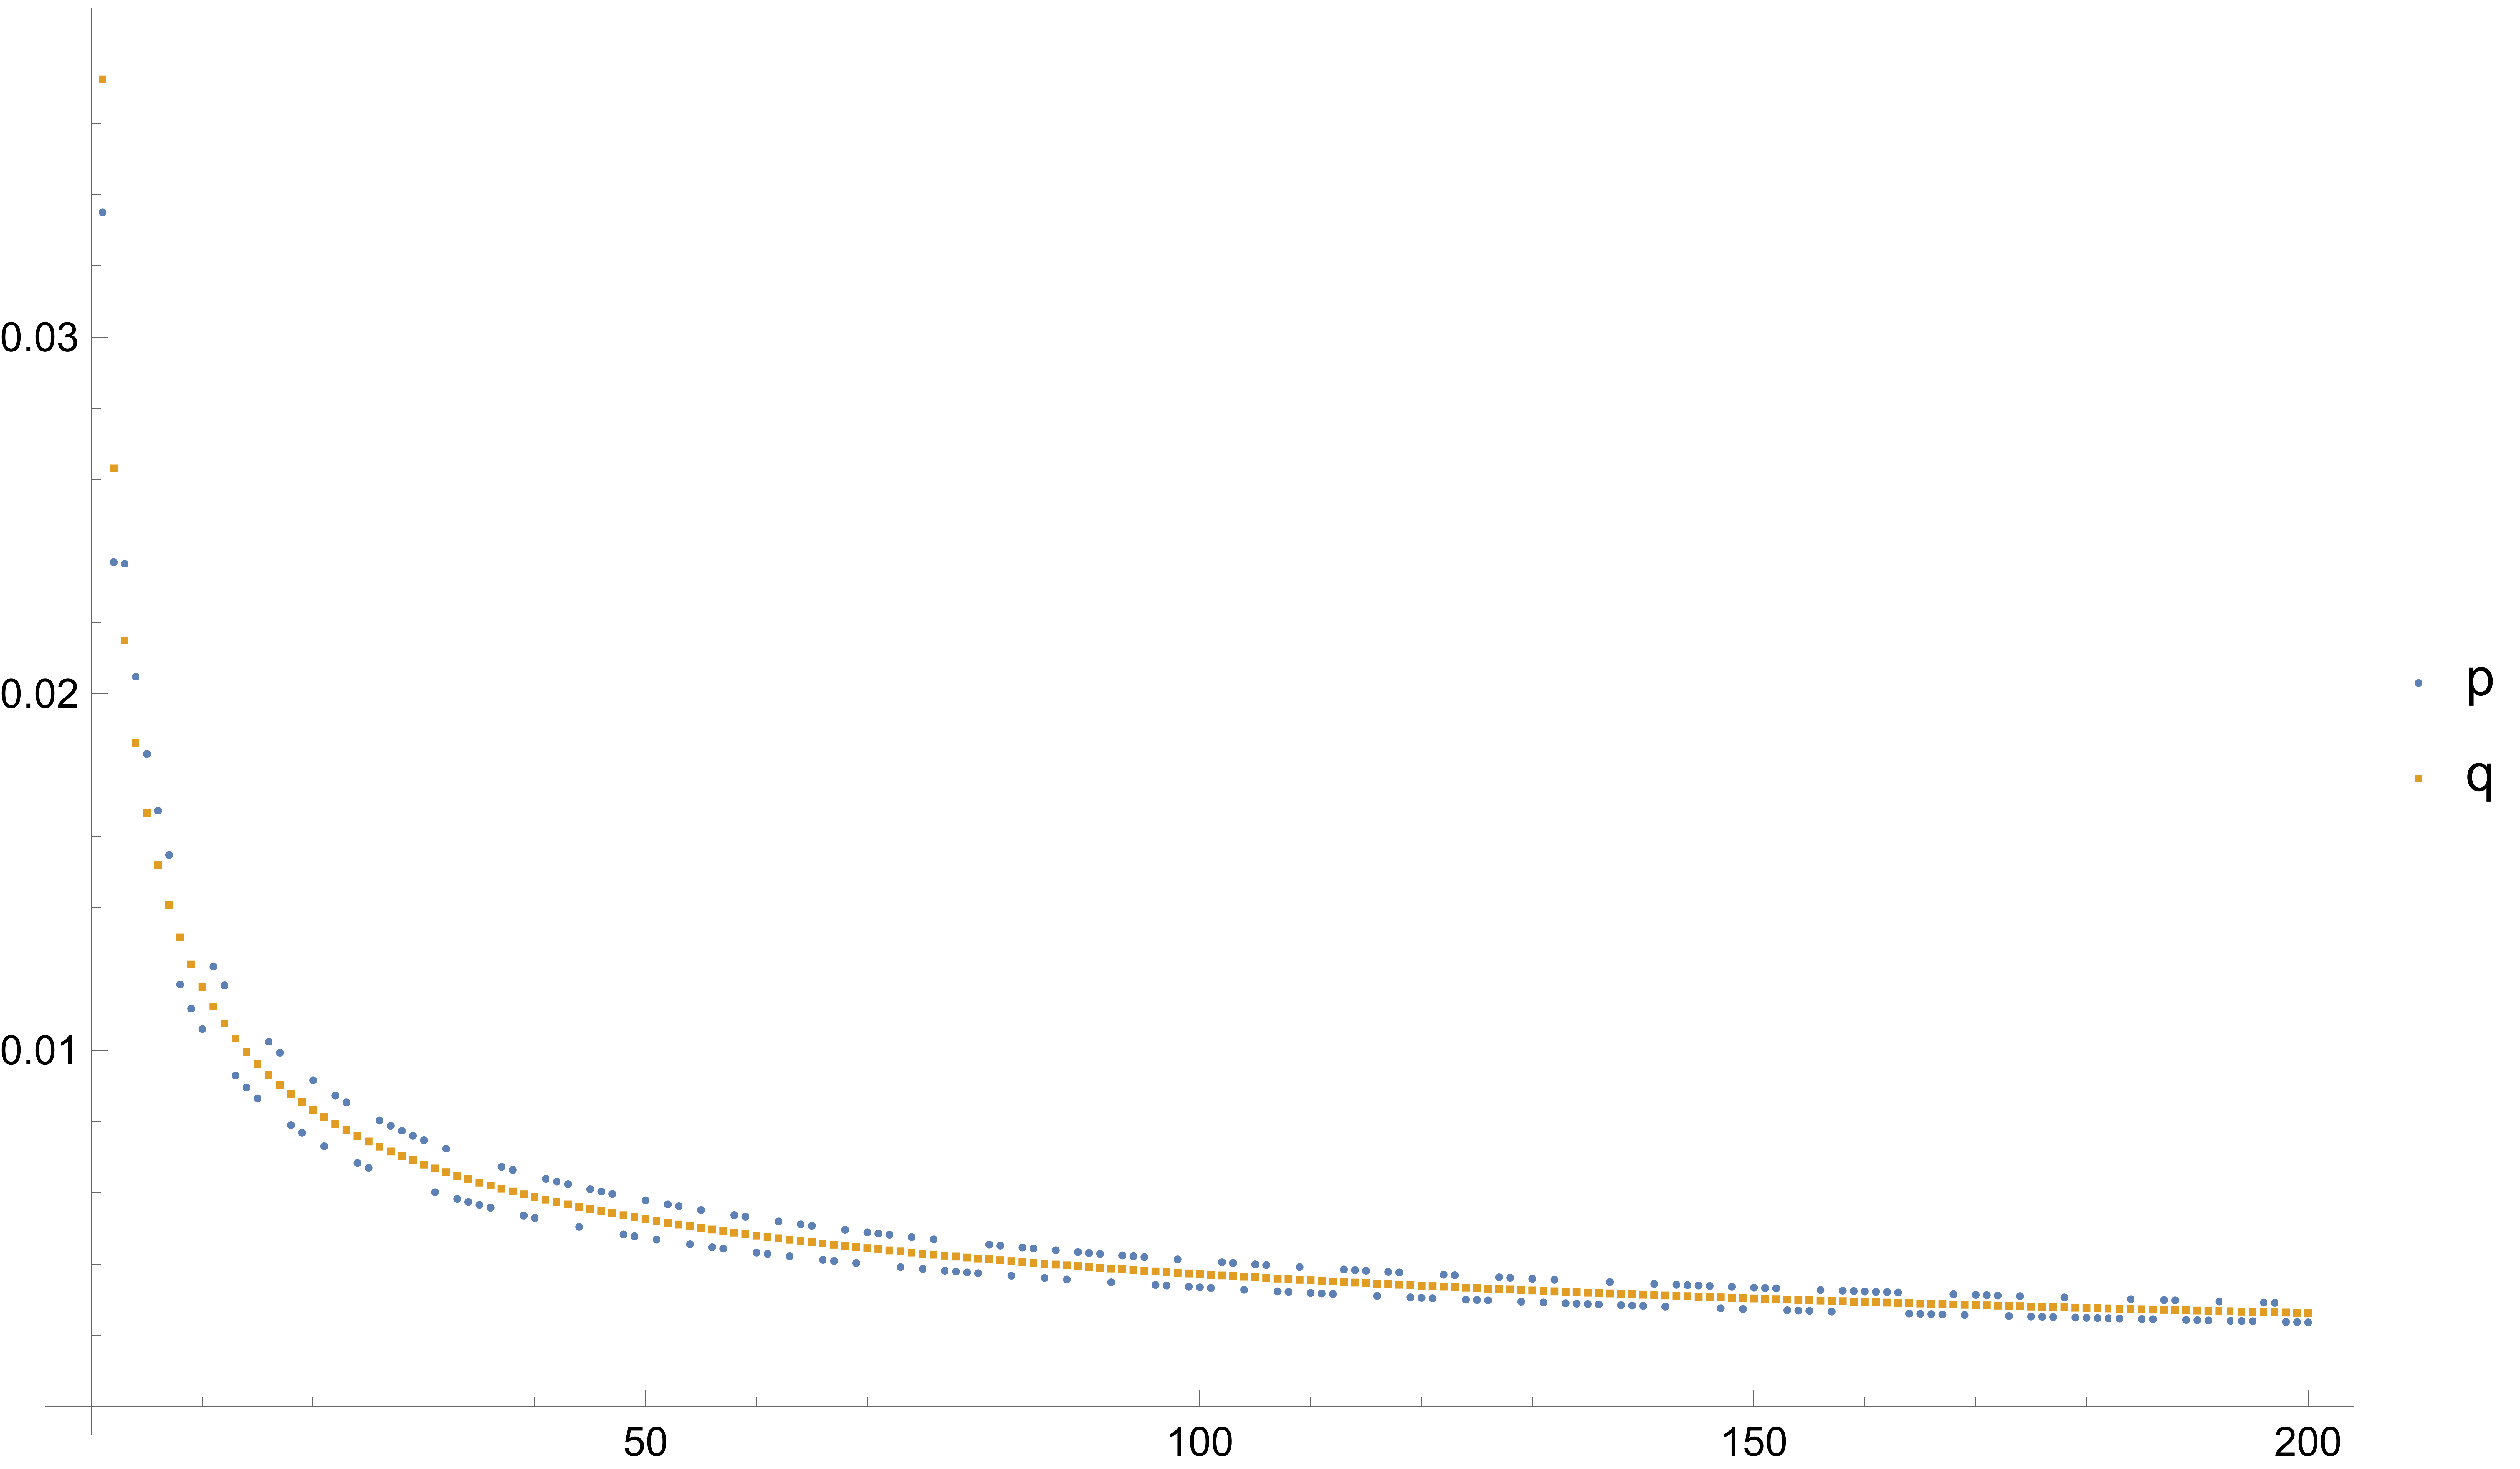
\includegraphics[width=1.0\textwidth]{figures/fig-lowerbound-zipf-pq}
	\caption{\label{fig:vv17:lb:zipf}Our reference $\q$ (Zipf distribution), along with a randomly chosen perturbation $\p$, here depicted for $\ab=200$, $\dst=1/10$.}
\end{figure}
%%%%%%%%%%%%%%%%%%%%%%%%%%%%%%%%%%%%%%%%%%%%%%%%%%%%%%%%%%%%%%%%%%%%%%%%%
While the second half (``tail'') of the distribution looks somewhat uniform (all probabilities between $\ab/2$ and $\ab$ are within a factor $\sqrt{2}$), the first half is clearly not, with the first few elements having much higher probability. Perturbing those heavy elements by the same relative amount as the rest, ``intuitively,'' is not a good idea, as it is easier to detect and can give away a lot more information. Instead, we will see what happens when we only perturb this somewhat-uniform tail of $\q$: define our $\alpha_i$'s by
\[
	\alpha_i \eqdef 
	\begin{cases}
		16\dst &\text{if } i \geq \frac{\ab}{2}\\
		0 &\text{ otherwise}
	\end{cases}
\]
In view of applying~\cref{theo:vv:lb}, we first check that the distance of our hard instances $\p_z$ to $\q$ will be at least $\dst$:
$
\max_{i} \alpha_i\q(i) = 16\dst\q(\ab/2) \ll \dst
$, and
\[
	\frac{1}{4}\sum_{i=1}^\ab \alpha_i\q(i) = 	\frac{4\dst}{H_{\ab,1/2}} \sum_{i=\frac{\ab}{2}}^\ab \frac{1}{\sqrt{i}} = 4\dst\Paren{1-\frac{H_{\frac{\ab}{2},1/2}}{H_{\ab,1/2}}} \geq 4\Paren{1-\frac{1}{\sqrt{2}}}\dst > \dst\,,
\]
so by~\cref{eq:vv:proba:far} the distance is fine. Turning to the sample complexity lower bound this will lead to, we compute
\[
	\sum_{i=1}^\ab \alpha_i^4 \q(i)^2 = \frac{(16\dst)^4}{H_{\frac{\ab}{2},1/2}^2}\sum_{i=\frac{\ab}{2}}^\ab \frac{1}{i} 
	= \frac{(16\dst)^4}{H_{\frac{\ab}{2},1/2}^2} \Paren{ H_{\ab} - H_{\frac{\ab}{2}} }
	\asymp \frac{\dst^4}{\ab}
\] 
since $H_{\ab} - H_{\ab/2} = \ln 2 + o(1)$. By~\cref{eq:vv:lb:samples}, this means we get a (tight) lower bound of $\Omega(\sqrt{\ab}/\dst^2)$ samples! All we needed to do was to restrict our perturbation to the ``near-uniform'' part of the reference distribution; crucially, this required the ability to choose different $\alpha_i$'s for different $i$, as allowed by~\cref{theo:vv:lb}.\medskip

To conclude this section, we will derive another corollary to~\cref{theo:vv:lb}, which provides the ``best'' perturbation possible for any given reference $\q$; that is, an optimal choice for the $\alpha_i$'s as a function of $\q$. Based on our previous example, we know that $\alpha_i$ somehow has to \emph{adapt} to $\q(i)$, to differentiate between the heavy elements and the ``near-uniform'' part of the distribution $\q$.

Now, on the one hand we want to establish as large a lower bound as possible, and so~\cref{eq:vv:lb:samples} says we should maximize
$
\sum_{i=1}^\ab \alpha_i^4\q(i)^2
$. On the other hand, for our lower bound to be meaningful, we also need our hard instances to be at distance $\dst$ from $\q$, and for that~\cref{eq:vv:proba:far} imposes the condition
$
\sum_{i=1}^\ab \alpha_i\q(i) \asymp \dst
$. Since
\begin{equation}
	\sum_{i=1}^\ab \alpha_i^4\q(i)^2 \leq \max_i \alpha_i^3\q(i) \cdot \sum_{i=1}^\ab \alpha_i\q(i)
\end{equation}
combining the two conditions leads us to try and maximize $\max_i \alpha_i^3\q(i)$, and the condition for equality in H\"older's inequality further suggests we should have $\alpha_i^3\q(i)$ constant; that is,
\begin{equation}
	\label{eq:vv:lb:intuition}
	\alpha_i \propto 1/\q(i)^{1/3}\,.
\end{equation}
We may not be able to do this exactly, as the theorem also requires that $\alpha_i \leq 1$, so we will have to cap our $\alpha_i$'s;  but this motivates the following idea. Without loss of generality, assume that $\q$ is non-increasing: $\q(1)\geq \q(2)\geq \dots\geq \q(\ab)$ (we can, since we know $\q$, and can permute the domain if we want) and $\dst\in(0,1/8]$; and assume, \emph{with} some loss of generality, that $\q(1)=\norminf{\q} \leq 1/2$. First, define $\alpha\geq 0$ as a value such that
\begin{equation}
	\label{eq:vv:lb:choice:alpha}
	\frac{1}{4}\sum_{i=2}^\ab \Paren{1\land \frac{\alpha}{\q(i)^{1/3}}}\q(i) = \dst
\end{equation}
where we start the summation at $i=2$ to (later) handle the (annoying) condition from~\cref{theo:vv:lb} on $\max_i \alpha_i\q(i)$, which will be $\alpha_1\q(1)$. To see why such a choice of $\alpha$ always exists, note that 
the LHS of~\cref{eq:vv:lb:choice:alpha} is continuous and non-decreasing in $\alpha$, equal to $0$ for $\alpha=0$, and goes to $\frac{1}{4}\sum_{i=2}^\ab \q(i) = \frac{1}{4}(1-\norminf{\q}) \geq \frac{1}{8}$ for $\alpha\to\infty$.

One we have this value $\alpha$, we can then set
\begin{equation}
	\label{eq:vv:lb:choice:alphai}
	\alpha_i =
	\begin{cases}
		1\land \frac{\alpha}{\q(i)^{1/3}} &\text{ if } 1\leq i\leq \ab\\
		\alpha_2\frac{\q(2)}{\q(1)} &\text{ if } i =1
	\end{cases}
\end{equation}
where the assumption that $\q$ is non-increasing implies that (i)~$\alpha_1\leq\alpha_2\leq \alpha_3\leq \dots \leq \alpha_\ab$, and (ii)~$\alpha_1\q(1)=\alpha_2\q(2)\geq \alpha_3\q(3)\geq \dots \geq \alpha_\ab\q(\ab)$ (since $\alpha_i\q(i) = \q(i)\land (\alpha\q(i)^{2/3})$).

\noindent Our (somewhat bizarre) choice of $\alpha_1$ is a technicality to ensure that
\[
	\max_i \alpha_i\q(i) = \alpha_1\q(1) = \frac{1}{2}(\alpha_1\q(1)+\alpha_2\q(2)) \leq \frac{1}{2}\sum_{i=1}^\ab \alpha_i\q(i)
\]
so that the condition of~\cref{theo:vv:lb} preceding~\cref{eq:vv:proba:far} is satisfied. Letting $L$ to be the largest value $i\geq 2$ such that $\alpha\q(i)^{-1/3} \leq 1$, we then can rewrite~\cref{eq:vv:lb:choice:alpha} as
\begin{equation}
	\label{eq:vv:lb:choice:alpha:2}
	\alpha\sum_{i=2}^L \q(i)^{2/3} + \sum_{i=L+1}^\ab \q(i) = 4\dst\,,
\end{equation}
from which $\alpha \leq 4\dst/\sum_{i=2}^L \q(i)^{2/3}$. Finally, recalling~\cref{eq:vv:lb:samples}, we bound
\begin{align}
	\sum_{i=1}^\ab \alpha_i^4\q(i)^2
	&\leq \sum_{i=2}^\ab \alpha_i^4\q(i)^2
	= \alpha^4\sum_{i=2}^L \q(i)^{2/3} + \sum_{i=L+1}^\ab \q(i)^2 \notag\\
	&\leq \alpha^3\Paren{\alpha\sum_{i=2}^L \q(i)^{2/3} + \sum_{i=L+1}^\ab \q(i) } \notag\\
	&= 4\dst \alpha^3 \tag{By~\cref{eq:vv:lb:choice:alpha:2}}\\
	&\leq \frac{(4\dst)^4}{\Paren{\sum_{i=2}^L \q(i)^{2/3}}^3}
\end{align}
where we used that $\q(i) \leq \alpha^3$ for all $i \geq L+1$ in the second inequality. Applying~\cref{theo:vv:lb} (along with the similar arguments as in the proof of~\cref{theo:uniformity:lb:vv}), what this shows is a lower bound of
\begin{equation}
	\label{eq:vv:lb:complicated}
	\bigOmega{ \frac{\Paren{\sum_{i=2}^L \q(i)^{2/3}}^{3/2}}{\dst^2}}
\end{equation}
samples to test identity to $\q$, where $L=L(\q,\dst)$ is defined above, and $\q$ satisfies $\norminf{\q}\leq 1/2$ and is (without loss of generality) assumed non-decreasing. This bound can seem quite daunting, due to the way $L(\q,\dst)$ is defined; fortunately, we can relax it a little to make it more interpretable (though technically looser). 

Observe that~\cref{eq:vv:lb:choice:alpha:2} also implies $\sum_{i=L+1}^\ab \q(i) \leq 4\dst$; thus, if we define $K=K(\q,\dst)$ as the largest integer such that $\sum_{i=K}^\ab \q(i) > 4\dst$, we are guaranteed that $K(\q,\dst)\leq L(\q,\dst)$ and therefore $\sum_{i=2}^K \q(i)^{2/3} \leq \sum_{i=2}^L \q(i)^{2/3}$. This leads to the following corollary:
\begin{theorem}
  \label{theo:2/3:lb:vv}
Given a probability distribution $\q\in\distribs{\ab}$, let $\tilde{\q}^{-\!\max}_{-4\dst}$ denote the vector obtained by seeing $\q$ as a vector in $[0,1]^\ab$, and removing (i)~its largest entry, and (ii)~its smallest entries, stopping just before the total removed exceeds $4\dst$. Then every testing algorithm for identity with reference $\q$ must have sample complexity $\ns(\ab,\dst,1/3) = \Omega(\lVert\tilde{\q}^{-\!\max}_{-4\dst}\rVert_{2/3}/\dst^2)$, provided that $\norminf{\q}\leq 1/2$ and $\dst\in(0,1/8]$.
\end{theorem}
\noindent One can check that this does retrieve the $\Omega(\sqrt{\ab}/\dst^2)$ testing lower bound both when (1)~$\q$ is the uniform distribution, (2)~$\q$ is the Zipf  distribution we saw in our earlier example\medskip.\exercise{Check it! (\cref{ex:2/3:lb:applications})}

%%%% Comment on uses beyond identity testing! E.g., LB for other problems.

Finally, it is worth mentioning that~\cref{theo:vv:lb} is not restricted to identity testing (although this is the application we detailed in this section). One can use it to establish indistinguishability results for other questions, focusing on the sample complexity lower bound it provides (\cref{eq:vv:lb:samples}) and possibly ignoring the distance part (\cref{eq:vv:proba:far}). For instance, it can be used to establish sample complexity lower bounds for testing in other norms than total variation distance, or to obtain lower bounds on estimating some parameter of interest.

%%%%%%%%%%%%%%%%%%%%%%%%%%%%%%%%%%%%%%%%%%%%%%%%%%%
\section{Proving hardness by reductions}
	\label{ssec:lb:reductions}
In this section, we will shift focus a little, and discuss how to \emph{leverage work (other) people did} in order to establish new sample complexity lower bounds. To illustrate the idea, consider the property $\property^{\searrow}=\cup_{\ab=1}^\infty \property^{\searrow}_\ab$ of \emph{monotone} (non-increasing) distributions,
\ie
\begin{equation}
\property^{\searrow}_\ab \eqdef \setOfSuchThat{ \p\in\distribs{\ab} }{ \p(1)\geq \p(2) \geq \dots \geq \p(\ab) }
\end{equation}
Say we want to test this property $\property^{\searrow}$: that is, given samples from a distribution over $\{1,2,\dots,\ab\}$, we want to test whether its pmf is non-increasing; more specifically, say we want to show it is not easy. We could try to use techniques from the previous subsections (though probably not directly those from~\cref{ssec:momentmatching}, as $\property^{\searrow}$ is most definitely not a symmetric property) to establish a sample complexity lower bound: this will require quite a bit of thinking and at least of few non-trivial computations.

But we have already shown (in a few different ways by now) that \emph{uniformity} testing had sample complexity $\Omega(\sqrt{\ab}/\dst^2)$. Can we somehow show that testing monotonicity is \emph{at least as hard}, and get the same lower bound without working much more? Enters the concept of \emph{reduction}, quite central to (theoretical) computer science. We already saw it in~\cref{ssec:l1:reduction}, when we used it to show how to use any uniformity testing algorithm for the more general problem of identity testing: that is, we described a reduction from uniformity to identity testing to get an algorithm (upper bound) for the latter, using an algorithm for the former. But every coin has two sides, and a reduction can be used to show lower bounds too!

Here's how. Imagine we had an ``efficient'' reduction from uniformity testing to monotonicity testing: given samples from an arbitrary distribution $\p\in\distribs{\ab}$, we can obtain samples from a distribution $\Phi(\p)\in\distribs{\ab'}$ such that (i)~$\Phi(\p)\in\property^{\searrow}_{\ab'}$ whenever $\p=\uniform_\ab$, and $\totalvardist{\Phi(\p)}{\property^{\searrow}_{\ab'}} > \dst'$ whenever $\totalvardist{\p}{\uniform_\ab} > \dst$. We allow the domain to change a little, from $\ab$ to some (not much larger) $\ab'$; and similarly for the distance parameter, originally $\dst$, which can become some other (not much smaller) value $\dst'$. See~\cref{fig:reduction:monotonicity} for a depiction.

\begin{figure}[htbp]\centering
\tikzset {_3eubqr20l/.code = {\pgfsetadditionalshadetransform{ \pgftransformshift{\pgfpoint{0 bp } { 0 bp }  }  \pgftransformrotate{0 }  \pgftransformscale{2.64 }  }}}
\pgfdeclarehorizontalshading{_y5uoy9rpz}{150bp}{rgb(0bp)=(0.99,0.97,0.93);
rgb(54.285714285714285bp)=(0.99,0.97,0.93);
rgb(61.96428571428571bp)=(0.98,0.95,0.95);
rgb(100bp)=(0.98,0.95,0.95)}
\tikzset{every picture/.style={line width=0.75pt}} %set default line width to 0.75pt        

\begin{tikzpicture}[x=0.75pt,y=0.75pt,yscale=-1.3,xscale=1.3]
%uncomment if require: \path (0,300); %set diagram left start at 0, and has height of 300

%Shape: Polygon Curved [id:ds24835565753561872] 
\draw  [xshift=-100pt,draw opacity=0.05,scale=0.85,yshift=20pt,xshift=-20pt][shading=_y5uoy9rpz,_3eubqr20l] (228.87,88.88) .. controls (266.87,64.88) and (266.87,111.88) .. (282.87,123.88) .. controls (298.87,135.88) and (360.87,96.88) .. (335.87,141.88) .. controls (310.87,186.88) and (389.87,249.88) .. (305.87,226.88) .. controls (221.87,203.88) and (251.87,247.88) .. (208.87,236.88) .. controls (165.87,225.88) and (201.87,193.88) .. (183.87,172.88) .. controls (165.87,151.88) and (157.87,118.88) .. (191.87,123.88) .. controls (225.87,128.88) and (190.87,112.88) .. (228.87,88.88) -- cycle ;
%Shape: Circle [id:dp2977666721327956] 
\draw  [draw opacity=0,scale=0.45,xshift=-91pt,yshift=153pt][fill={rgb, 255:red, 253; green, 170; blue, 30 }, fill opacity=0.7 ][general shadow={fill={rgb, 255:red, 245; green, 166; blue, 35 },shadow xshift=0pt,shadow yshift=0pt, opacity=0 }] (242,165.5) .. controls (248,147) and (253,132) .. (271.5,132) .. controls (290,132) and (305,147) .. (308,165.5) .. controls (310,184) and (290,199) .. (271.5,199) .. controls (253,199) and (238,184) .. (242,165.5) -- cycle ;
%Shape: Circle [id:dp2977666721327956] 
\draw  [draw opacity=0.05,scale=0.25,xshift=0pt,yshift=375pt][fill={rgb, 255:red, 253; green, 170; blue, 30 }, fill opacity=0.99 ][general shadow={fill={rgb, 255:red, 245; green, 166; blue, 35 },shadow xshift=0pt,shadow yshift=0pt, opacity=0 }] (242,165.5) .. controls (248,147) and (253,132) .. (271.5,132) .. controls (290,132) and (305,147) .. (308,165.5) .. controls (310,184) and (290,199) .. (271.5,199) .. controls (253,199) and (238,184) .. (242,165.5) -- cycle ;
%Shape: Ellipse [id:dp5805520465941827] 
\node at (50,120) (nodedistribs) {$\distribs{\ab}$};
\node at (90,145) (nodefar) {};
\node at (60,175) (nodeeps) {\scriptsize$\dst$};
\node at (70,168) (nodepropertyunif) {$\uniform_{\ab}$};
\node at (65,168) (nodepropertyunifstartarrow) {};

%%%%%%%%%%%%%%%%%%%%%%%%%%%%%%%%%%%%%%%%%%%%%%%%%%%%%%%%%%%%%%%%%%%%


%Shape: Polygon Curved [id:ds24835565753561872] 
\draw  [draw opacity=0.05][shading=_y5uoy9rpz,_3eubqr20l] (228.87,88.88) .. controls (266.87,64.88) and (266.87,111.88) .. (282.87,123.88) .. controls (298.87,135.88) and (360.87,96.88) .. (335.87,141.88) .. controls (310.87,186.88) and (389.87,249.88) .. (305.87,226.88) .. controls (221.87,203.88) and (251.87,247.88) .. (208.87,236.88) .. controls (165.87,225.88) and (201.87,193.88) .. (183.87,172.88) .. controls (165.87,151.88) and (157.87,118.88) .. (191.87,123.88) .. controls (225.87,128.88) and (190.87,112.88) .. (228.87,88.88) -- cycle ;
%Shape: Circle [id:dp2977666721327956] 
\draw  [draw opacity=0][fill={rgb, 255:red, 253; green, 170; blue, 30 }  ,fill opacity=0.70 ][general shadow={fill={rgb, 255:red, 245; green, 166; blue, 35 },shadow xshift=0pt,shadow yshift=0pt, opacity=0 }] (242,165.5) .. controls (248,147) and (253,132) .. (271.5,132) .. controls (290,132) and (305,147) .. (308,165.5) .. controls (310,184) and (290,199) .. (271.5,199) .. controls (253,199) and (238,184) .. (242,165.5) -- cycle ;
%Shape: Circle [id:dp2977666721327956] 
\draw  [draw opacity=0.05, scale=0.8,xshift=51pt,yshift=31pt][fill={rgb, 255:red, 253; green, 170; blue, 30 }  ,fill opacity=0.99 ][general shadow={fill={rgb, 255:red, 245; green, 166; blue, 35 },shadow xshift=0pt,shadow yshift=0pt, opacity=0 }] (242,165.5) .. controls (248,147) and (253,132) .. (271.5,132) .. controls (290,132) and (305,147) .. (308,165.5) .. controls (310,184) and (290,199) .. (271.5,199) .. controls (253,199) and (238,184) .. (242,165.5) -- cycle ;
%Shape: Ellipse [id:dp5805520465941827] 
\node at (240,120) (nodedistribsprime) {$\distribs{\ab'}$};
\node at (220,170) (nodefarprime) {};
\node at (245,175) (nodeepsprime) {\scriptsize$\dst'$};
\node at (275,165) (nodeproperty) {$\property^{\searrow}_{\ab'}$};



\draw [dotted,->] (nodefar) to  [out=-25,in=225] (nodefarprime);
\draw [dotted,->] (nodepropertyunifstartarrow) to [out=45,in=100] (nodeproperty);
\end{tikzpicture}
\caption{Illustration of what a reduction from uniformity testing to monotonicity testing is. The uniform distribution is mapped to some monotone distribution, while distributions far from uniform are mapped to distributions far from monotone. (Things that are neither uniform nor far from it can be mapped to anything.)\label{fig:reduction:monotonicity}}
\end{figure}
\noindent Then, any algorithm $\Tester$ for testing $\property^{\searrow}$ (with parameters $\ab',\dst'$) can be used to test uniformity (with parameters $\ab,\dst$): convert the samples from $\p\in\distribs{\ab}$ to samples from $\Phi(\p)\in\distribs{\ab'}$, run $\Tester$ on them, and output what this tester returns. Which is great\dots except that we know that $\Omega(\sqrt{\ab}/\dst^2)$ samples are required for the latter task; so the sample complexity $\ns$ of $\Tester$ must satisfy $\ns(\ab',\dst',1/3) = \Omega(\sqrt{\ab}/\dst^2)$. We get a lower bound! Whose meaningfulness, of course, depends a lot on how $\ab'$ and $\dst'$ are related to $\ab$ and $\dst$.\smallskip

Let us look at an example, to make things more concrete. Consider the following (randomized) mapping $\Psi\colon[\ab]\to[2\ab]$: 
\begin{description}
	\item[$\Psi$:] Given $i \in [\ab]$, return $i$ with probability $\frac{1}{2}$ and $\ab+i$ otherwise.
\end{description}
Applying this to a sample from a probability distribution $\p\in\distribs{\ab}$ results in a sample from $\Phi(\p)$ over $\ab'\eqdef2\ab$ (where $\Phi\colon\distribs{\ab}\to\distribs{\ab'}$), given by
\begin{equation}
	\label{eq:reduction:monotonicity}
	\Phi(\p)(i) = \frac{1}{2}\p(i\bmod\ab)
\end{equation}
which ``duplicates the domain and puts two contiguous copies of $\p$ next to each other.'' Why is it a good thing to consider? For a start, if we apply this to the uniform distribution $\uniform_\ab$, we end up with $\Phi(\uniform_\ab) = \uniform_{2\ab}$, the uniform distribution on our new domain, which is definitely in $\property^{\searrow}_{2\ab}$ (the uniform distribution may not be the most interesting monotone distribution, but it is a monotone distribution nonetheless). So this fits at least half the bill: as you will show in~\cref{ex:reduction:monotone},\exercise{Show this.} it also fits the other half: distributions which are $\dst$-far from uniform are mapped to distributions $\dst'$-far from uniform, where $\dst'\eqdef \dst/2$.

\begin{figure}[htbp]\centering
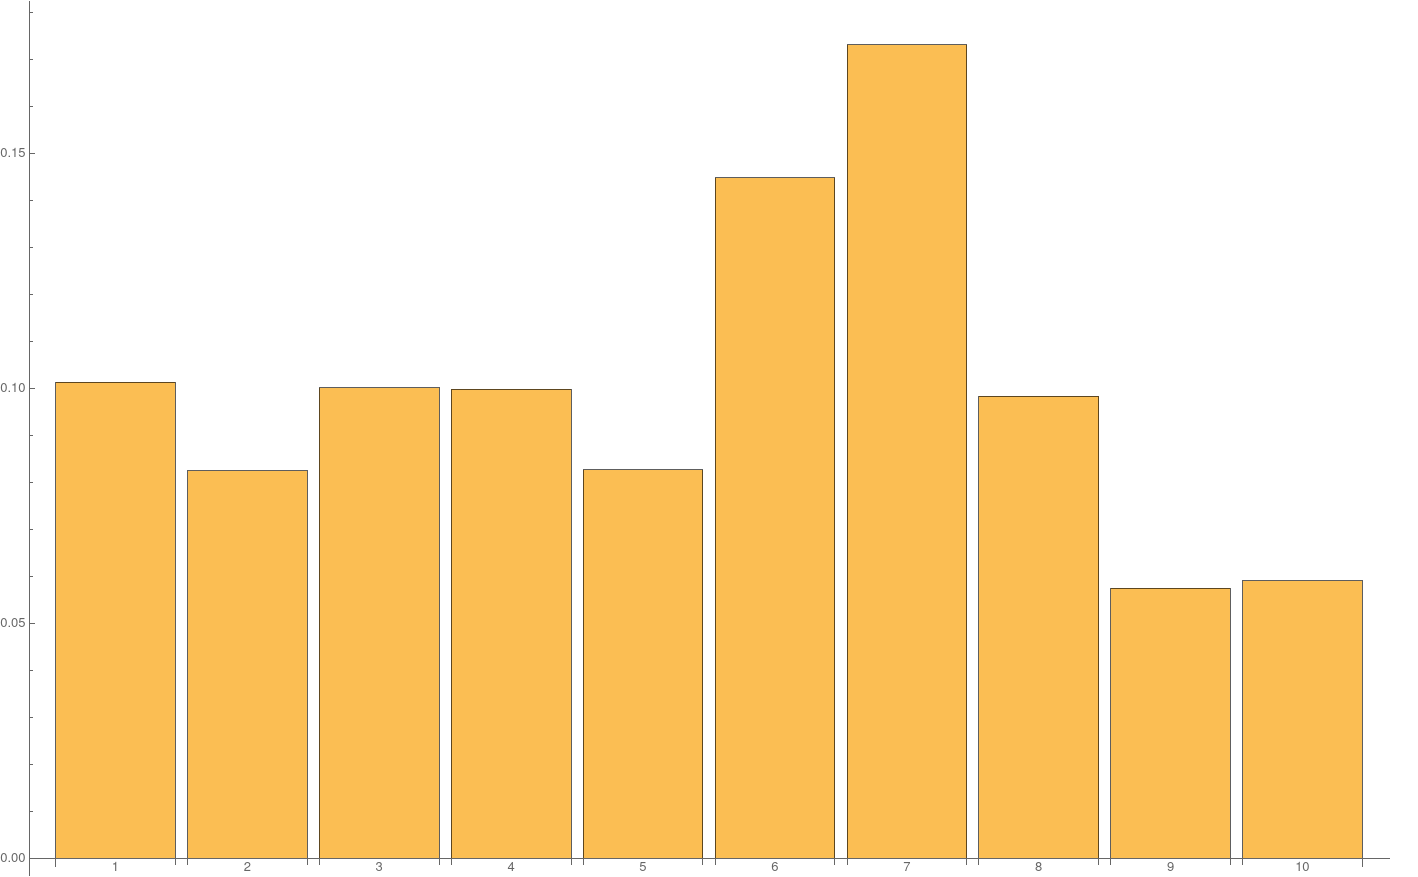
\includegraphics[width=.45\textwidth]{figures/fig-reduction-uniformity}\hfill
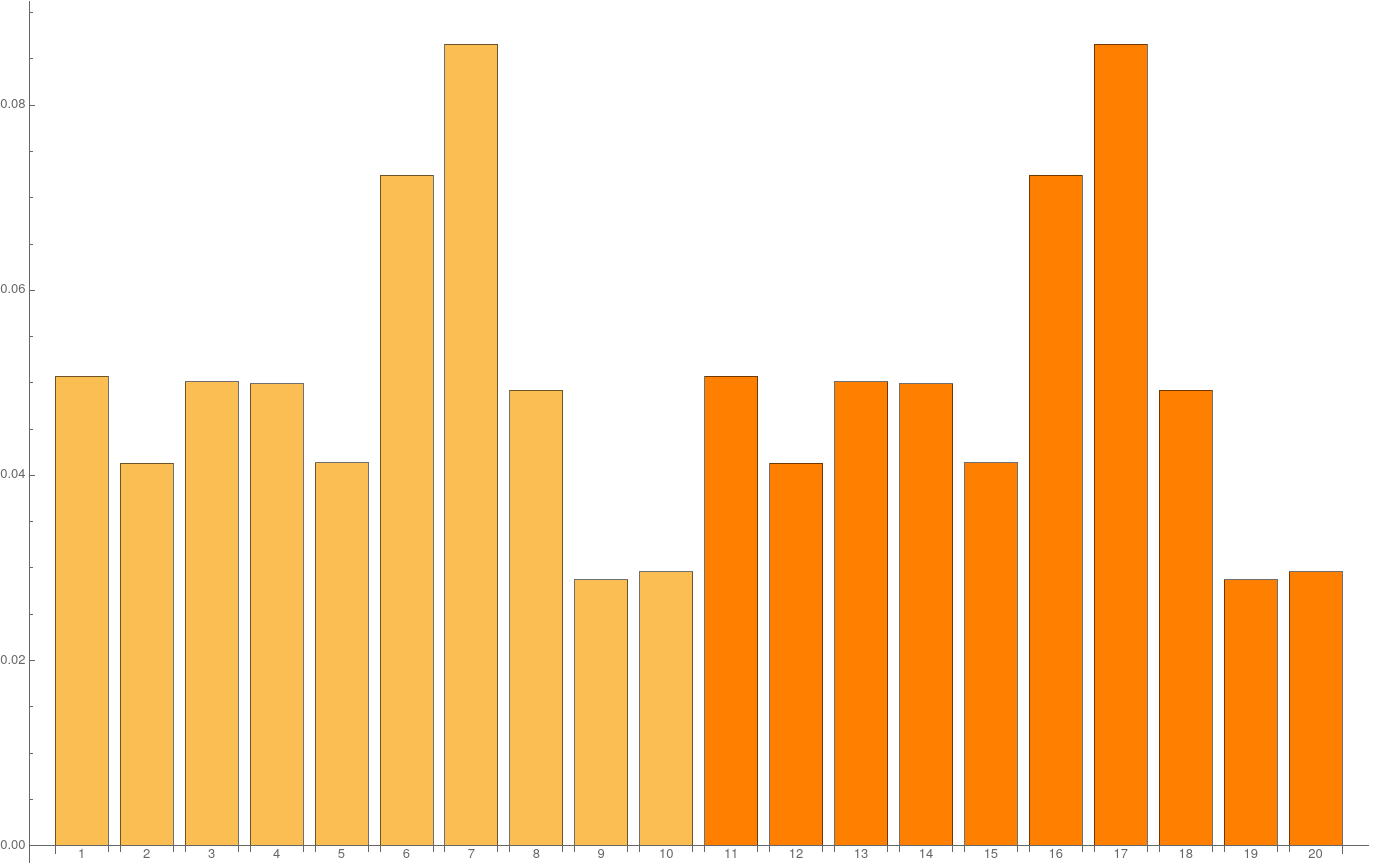
\includegraphics[width=.45\textwidth]{figures/fig-reduction-uniformity2}
\caption{An example of the reduction outlined above, with a distribution $\p$ over a domain of size $\ab=20$ (left) and the resulting $\Phi(\p)$ on a domain of size $\ab'=2\ab=40$ on the right.\label{fig:reduction:monotonicity:example}}
\end{figure}
By the above discussion, the lower bound on uniformity testing directly implies that monotonicity testing with parameters $2\ab$ and $\dst/2$ must have sample complexity $\Omega(\sqrt{\ab}/\dst^2)$. Since constant factors are just constant factors, this leads to the following:
\begin{theorem}
	\label{theo:lb:testing:monotonicity}
Every testing algorithm for $\property^{\searrow}$ (monotonicity) must have sample complexity $\ns(\ab,\dst,1/3) = \Omega(\sqrt{\ab}/\dst^2)$.
\end{theorem}
\noindent(As a side note, this is known to be tight, at least for $\dst \gg \sqrt{\log\ab}/\ab^{1/4}$.) Crucially, reductions comes with another advantage: if we were to introduce another parameter (focusing on the dependence on $\errprob$, for instance), or work with constrained measurements as in~\cref{chap:constrained}, then as long as our reduction goes through in the setting considered, we only need to derive the uniformity testing lower bound in that setting to immediately get the corresponding lower bound for monotonicity testing as well. As said earlier, reductions are great to avoid unnecessary work!

\paragraph{A general result.} The above reduction was quite specific to monotonicity testing: ideally, we would like more general statements, allowing us to derive as many lower bounds as possible while having to think as little as possible. In the rest of this section, we are going to describe such a result, which can be seen as some converse to the ``testing-by-learning'' baseline from~\cref{lemma:learning:baseline}. The high-level idea is as follows: suppose we have two properties $\property' \subseteq \property$, and we know that $\property'$ is hard to test. Then we want to conclude that $\property$, too, is hard to test~--~at least as hard as $\property'$. (In our earlier example, $\property'$ was uniformity, and $\property$ monotonicity: since the uniform distribution is monotone, the inclusion indeed holds.)

The issue with this conclusion, however, \emph{is that it is not true.} One can come up with very simple examples showing it: taking $\property_\ab = \distribs{\ab}$, for example (the trivial property containing all discrete distributions) and $\property'_\ab=\{\uniform_\ab\}$, we clearly have $\property'_\ab \subseteq \property_\ab$, yet $\property_\ab$ can be tested with exactly 0 samples~--~while $\property'_\ab$ requires $\Omega(\sqrt{\ab}/\dst^2)$.

Still, in that counterexample, the property $\property$ itself is ginormous (all distributions!), which somewhat explains the issue: in contrast, the property $\property^{\searrow}$ of monotone distributions was much smaller. If we restrict the statement to ``simple enough'' properties, then maybe the statement will hold? \textit{E.g.}, what about properties which can be \emph{learned} efficiently?  
As we will see momentarily, this is indeed the case, albeit for a very specific sense of ``learning'' we first need to introduce.

\begin{definition}[Agnostic learning]
	A class $\class=\bigcup_{\ab=1}^\infty \class_\ab$ is said to be \emph{agnostically learnable} with sample complexity $\ns(\ab,\dst,\errprob)$ if there is an algorithm which, given $\ns=\ns(\ab,\dst,\errprob)$ \iid samples from an unknown \emph{arbitrary} distribution $\p\in\distribs{\ab}$, outputs a distribution $\hat{\p}$ such that
	\[
		\totalvardist{\p}{\hat{\p}} \leq C\cdot \inf_{\q\in\class_\ab} \totalvardist{\p}{\q} + \dst
	\]
with probability at least $1-\delta$, where $C\geq 1$ is an absolute constant.
\end{definition}
In other terms, an agnostic learning algorithm works even in the unrealizable setting (when $\p\notin\class_\ab$), and its output is ``nearly as good'' as the best candidate from $\class_\ab$ would be. The main result of this section is the following theorem, which roughly states that ``if a property is easy to learn, then it is as hard to test as its hardest sub-property:''
\begin{theorem}[Hardness by Reduction]\label{theo:hardness:subclass}
  Fix any property $\property$, and suppose there exists $\property'\subseteq \property$ such that the following holds.
  \begin{enumerate}
    \item\label{theo:hardness:subclass:item1} Agnostic learning of $\property$ (with a given ``agnostic constant'' $C\geq 1$) has sample complexity at most $\ns_{\mathcal{L}}(\ab,\dst,\delta)$;
    \item\label{theo:hardness:subclass:item2} Testing $\property'$ has sample complexity at least $\ns_{\mathcal{T}}(\ab,\dst,\errprob)$;
    \item\label{theo:hardness:subclass:item3} There exists a range of parameters $\ab,\dst,\errprob$ for which learning $\property$ is easier than testing $\property'$: 
    	\[
    		\ns_{\mathcal{L}}(\ab,C\dst,\errprob) \leq \frac{1}{2}\ns_{\mathcal{T}}(\ab,3C\dst,2\errprob)
    	\]
  \end{enumerate}
  Then, for $\ab,\dst,\errprob$ in that range of parameters, every testing algorithm for $\property$ must have sample complexity at least $\frac{1}{2}\ns_{\mathcal{T}}(\ab,3C\dst,2\errprob)$.
\end{theorem}
\begin{proof}
The idea of the proof is quite simple: suppose we have a testing algorithm $\Algo$ for $\property$ with sample complexity $\ns_\Algo(\ab,\dst,\errprob)$, and let $\Learner$ be the agnostic learning algorithm for $\property$ with sample complexity $\ns_{\mathcal{L}}(\ab,\dst,\errprob)$ promised by~\cref{theo:hardness:subclass:item1}. Then we can combine both to obtain a testing algorithm for $\property'$: but since $\property'$ is hard to test, this testing algorithm cannot be \emph{too} sample-efficient (it must take at least $\ns_{\mathcal{T}}$ samples), giving us a lower bound $\ns_\Algo+\ns_\Learner \geq \ns_{\mathcal{T}}$. (Note that we only care about sample complexity, and do not make any assumption on computational efficiency.)

\noindent In more detail, consider the following testing algorithm $\Algo'$ for $\property'$: on input $\ab,\dst,\errprob$,
\begin{itemize}
	\item Run $\Algo$ with parameters $\ab,\dst/(3C),\errprob/2$; let $b\in\{\reject,\accept\}$ be the result.
	\item Run $\Learner$ with parameters $\ab,\dst/3,\errprob/2$; let $\hat{\p}$ be the output.
	\item Check whether $\totalvardist{\hat{\p}}{\property'} \leq \dst/3$; let $b'\in\{\reject,\accept\}$ indicate the result (this is purely computational and requires no samples from $\p$).
	\item Return $b\land b'$ (\ie \accept if, and only if, both $b$ and $b'$ were \accept).
\end{itemize}
Since both $\Algo$ and $\Learner$ were run with error probability $\errprob/2$, by a union bound they are simultaneously correct with probability at least $1-\errprob$. Assume hereafter this event holds.
\begin{itemize}
\item If $\p\in\property'$, then \textit{a fortiori} $\p\in\property$, and $\Algo$ returns $b=\accept$. Moreover, $\totalvardist{\p}{\hat{\p}} \leq C\cdot 0 + \dst/3 = \dst/3$, so $b'=\accept$ as well, and overall $\Algo'$ returns \accept.
\item Let us now argue the ``soundness.'' Suppose that $\Tester'$ returns $\accept$: this means that $b=\accept$, and so since $\Algo$ is a testing algorithm for $\property$ we must have $\totalvardist{\p}{\property} \leq \dst/(3C)$. But then, since $\Learner$ is an agnostic learner for $\property$, we get $\totalvardist{\p}{\hat{\p}} \leq C\cdot \totalvardist{\p}{\property} + \dst/3 \leq 2\dst/3$. And finally, since the last check was successful as well ($b'=\accept$), we have that $\totalvardist{\hat{\p}}{\property'} \leq \dst/3$. By the triangle inequality, it follows that
\[
	\totalvardist{\p}{\property'} \leq \totalvardist{\p}{\hat{\p}}+\totalvardist{\hat{\p}}{\property'} \leq \dst\,.
\]
By contrapositive, if $\totalvardist{\p}{\property'} > \dst$ then it must be the case that $\Tester'$ returns $\reject$.
\end{itemize}
So $\Tester'$ is a \textit{bona fide} testing algorithm for $\property'$, and its sample complexity is
\[
	\ns'(\ab,\dst,\errprob) = \ns_\Algo(\ab,\dst/(3C),\errprob/2) + \ns_{\mathcal{L}}(\ab,\dst/3,\errprob/2)
\]
or, reparameterizing, 
\[
	\ns'(\ab,3C\dst,2\errprob) = \ns_\Algo(\ab,\dst,\errprob) + \ns_{\mathcal{L}}(\ab,C\dst,\errprob)\,.
\]
But since we know by~\cref{theo:hardness:subclass:item2} that $\property'$ is hard to test, we must then have
\[
	\ns_\Algo(\ab,\dst,\errprob) + \ns_{\mathcal{L}}(\ab,C\dst,\errprob) \geq \ns_{\mathcal{T}}(\ab,3C\dst,2\errprob)
\]
which by~\cref{theo:hardness:subclass:item3} implies $\ns_\Algo(\ab,\dst,\errprob) \geq \ns_{\mathcal{T}}(\ab,3C\dst,2\errprob)$, and proves the theorem.
\end{proof}

With this theorem in hand, proving a sample complexity lower bound for a given property $\property$ boils down to scouring the literature to check if (1)~$\property$ is easy to learn, and (2)~something (anything!) inside $\property$ is known to be hard to test. Note that the result may not always be an \emph{optimal} lower bound; but it often gets quite close to it, and is a simple and valuable starting point.\smallskip

To conclude, let us see a direct application of this theorem to the property $\property^{\searrow}$. We can use the fact that monotone distributions can be agnostically learned with $O(\log(1+\dst\ab)/\dst^3)$ samples~\citep{Birge87,DDS:12} along with our uniformity testing lower bound (taking $\property'_\ab \eqdef \{\uniform_\ab\}$). This lets us derive the same $\Omega(\sqrt{\ab}/\dst^2)$ sample complexity lower bound for testing $\property^{\searrow}$ as in~\cref{theo:lb:testing:monotonicity}, with the additional (small) restriction $\dst \gg (\log\ab)/\sqrt{\ab}$. Here again, we relied on the uniformity testing lower bound: it is worth pointing out that we can (and sometimes must) use other ``hard-to-test'' sub-properties than uniformity! We will see such an example in~\cref{ex:testing:pbd}, where you will be asked to prove a lower bound on testing ``Poisson Binomial Distributions.''

% Exercise VV17 for Binomial + this -> LB for PBDs
%%%%%%%%%%%%%%%%%%%%%%%%%%%%%%%%%%%%%%%%%%%%%%%%%%%
%%\section{Application: distributed inference}

%%%%%%%%%%%%%%%%%%%%%%%%%%%%%%%%%%%%%%%%%%%%%%%%%%%
\section{Historical notes}

The contents of~\cref{ssec:ingster} (mostly) follow the exposition of~\citet{Pollard:2003} of the celebrated work of Le Cam (\eg~\citet{LeCam73}). The $\chi^2$ method described (\cref{lemma:ingster}) is, to the best of the author's knowledge, due to Ingster, and often referred to as the Ingster--Suslina method after~\citep{IngsterS03}.~\cref{ssec:dk16} (mostly) follows the Fano-based framework of~\citet{DiakonikolasK16}, with some simplifications and (hopefully not) the occasional new typo.

The results discussed in~\cref{ssec:momentmatching} are due to~\citet{Valiant:11}; those from~\cref{ssec:vv:instancebyinstance} first appeared in~\citet{VV:14:FOCS}, before the journal version~\citep{ValiantV17}.

The reduction-based method from~\cref{ssec:lb:reductions} was introduced in~\citet{CDGR:16} (the journal version appearing later as~\citep{CDGR:17:journal}), which also includes a variant for tolerant testing. This is not the only type of reduction-based method known; for a different flavour entirely (reduction from communication complexity), the reader is encouraged to consult~\citet{BlaisCG19}.

Importantly, all methods and results covered in this chapter focused on minimax \emph{testing} lower bounds. While they can also be used to establish sample complexity lower bounds for estimation questions (since, essentially, ``learning is harder than testing,'' as briefly discussed in~\cref{chap:what}), there are many situations where the bounds obtained by these methods will not be optimal for estimation tasks. The reader interested in estimation \textit{versus} testing lower bound methods is referred to the foundational paper of~\citet{Yu97}.

%%%%%%%%%%%%%%%%%%%%%%%%%%%%%%%%%%%%%%%%%%%%%%%%%%%%%%%%%%%%%%%%%%%%%%%%%
%%%%%%%%%%%%%%%%%%%%%%%%%%%%%%%%%%%%%%%%%%%%%%%%%%%%%%%%%%%%%%%%%%%%%%%%%
\section{Exercises}

\begin{question}\label{exo:deriving:dep:delta:lb}
Combine (the second part of)~\cref{app:distances:bh} with (the first part of)~\cref{lemma:kl:chi2} to obtain~\cref{eq:bound:ingster:mgf:uniformity} from~\cref{eq:lecam}. Use it to derive~\cref{theo:uniformity:lb:ingster:with:delta}.
\end{question}

\begin{question}\label{exo:notrealproba:lb}
Let $\p$ be a measure (not necessarily a probability measure) such that the $\lp[1]$ distance between $\p$ and $\property_\ab$ satisfies $\lp[1](\p,\property_\ab)>2\dst$, and $1/2\leq \normone{\p} \leq 3/2$. Defining $\p' \eqdef \p/\normone{\p}$ (an actual probability distribution), provide a lower bound on $\totalvardist{\p}{\property_\ab}$. Moreover, show that obtaining $\ns$ ``samples'' from the Poisson process with measure $\p$ is equivalent to getting $\poisson{\ns\normone{\p}}$ samples from the distribution $\p'$.

Conclude with how one could use a testing algorithm $\Algo$ for property $\property_\ab$ given $\poisson{\ns}$ samples (\ie in the Poissonized sampling model) to distinguish between two families of measures (\yes- and \no-instances) far in $\lp[1]$ distance, thus justifying the relaxed assumption from~\cref{ssec:dk16}.
\end{question}

\begin{question}[$\star$]\label{exo:paninski:mi:lb}
Recall that we defined the \no-instances in~\cref{ssec:dk16} by~\cref{eq:notpaninski:construction} (measures, instead of \emph{bona fide} probability measures) in order to guarantee mutual independence of $\occur_1,\dots,\occur_\ab$ (conditioned on $\mathbf{b}$. Check the argument to see which part of the argument would fail if we had used~\cref{eq:paninski:construction} instead. Then, modify the argument to fix this, and obtain the same sample complexity lower bound. \textit{(Hint: we still have mutual independence of the $\ab/2$ random variables $(\occur_1, \occur_2),\dots,(\occur_{\ab-1}, \occur_\ab)$ conditioned on $\mathbf{b}$. Establish the analogue of~\cref{eq:mutualinfobound} with $\occur_1=j,\occur_2=\ell$ instead of $\occur_1=j$, and proceed from there.}
\end{question}

\begin{question}\label{ex:2/3:lb:applications}
Verify that applying~\cref{theo:2/3:lb:vv} to (i)~the uniform distribution $\uniform_\ab$ and (ii)~the ``Zipf'' distribution $\q\in\distribs{\ab}$ such that $\q(i) \propto 1/\sqrt{i}$ leads, in both cases, to an $\Omega(\sqrt{\ab}/\dst^2)$ sample complexity lower bound for identity testing.
\end{question}

\begin{question}\label{exo:reexpress:algos:frequency:only}
Check that you can express several of the algorithms in~\cref{sec:uniformity} as a function of $\freq$ only (as defined in~\cref{ssec:momentmatching}). Specifically, verify this for~\cref{algo:collision-based,algo:unique-elements,algo:empirical:plugin}. Verify this also for~\cref{algo:chisquare}, keeping in mind that this algorithm was stated and analyzed in the Poissonized setting: what does it change?
\end{question}
\begin{question}[$\star$]\label{ex:reduction:monotone}
  Prove that the mapping $\Phi$ defined in~\cref{eq:reduction:monotonicity} does satisfy the requirements of a reduction, for $\ab'=2\ab$ and $\dst'=\dst/2$. That is, if $\p\in\distribs{\ab}$ is $\dst$-far from $\uniform_\ab$, then $\Phi(\p)\in\distribs{2\ab}$ is $\dst'$-far from every distribution $\q\in\property^{\searrow}_{2\ab}$. \textit{(Hint: for any given monotone $\q$, analyse the distance $\totalvardist{\Phi(\p)}{\q}$ according to whether $\q(\ab) > 1/(2\ab)$ or not, relating this to the set $S\subseteq[\ab]$ on which $\p$ is greater than $\uniform_\ab$.)} Moreover, show that this loss by a factor $1/2$ in the distance is necessary.
\end{question}
\iffalse %%%%%%%%%%% Hide answer
\begin{proof}[Solution of~\cref{ex:reduction:monotone}]
Fix any $\p\in\distribs{\ab}$ such that $\totalvardist{\p}{\uniform_\ab}>\dst$, and let $S\subseteq [\ab]$ the set which witnesses it:
$S\eqdef \setOfSuchThat{ 1\leq i\leq \ab }{\p(i)> 1/\ab }$ 
which satisfies 
\[
	\p(S)-\uniform_\ab(S) = \uniform_\ab([\ab]\setminus S)- \p([\ab]\setminus S) >\dst
\]
Further define $T \eqdef [\ab]\setminus S \subseteq \{1,2,\dots,\ab\}$, and $S+\ab = \setOfSuchThat{i+\ab}{i\in S} \subseteq \{\ab+1,\dots,2\ab\}$. 
By definition of $\Phi(\p)$, we then have
\[
	\uniform_{2\ab}(T)-\Phi(\p)(T)=\Phi(\p)(S+\ab)-\uniform_{2\ab}(S+\ab)= \frac{1}{2}(\p(S)-\uniform_\ab(S)>\frac{\dst}{2}\,.
\]
Now, fix any monotone distribution $\q\in\property^{\searrow}_{2\ab}$. We have two cases:
\begin{itemize}
\item If $\q(\ab) > 1/(2\ab)$, then, since $\q$ is monotone, $\q(i) > 1/(2\ab)$ for every $i \leq \ab$. This implies
\[
	\q(T)-\Phi(\p)(T) \geq \uniform_{2\ab}(T)-\Phi(\p)(T) > \frac{\dst}{2}
\]
\item If $\q(\ab) \leq 1/(2\ab)$, then $\q(i) \leq 1/(2\ab)$ for every $i \geq \ab$. This implies
\[
	\Phi(\p)(S+\ab)-\q(S+\ab) \geq \Phi(\p)(S+\ab)-\uniform_{2\ab}(S+\ab) > \frac{\dst}{2}
\]
\end{itemize}
This shows that $\totalvardist{\Phi(\p)}{\q} > \dst/2$. For the ``necessary'' part, consider $\p$ such that $\p(1)=1$.
\end{proof}
\fi  %%%%%%%%%%% End of hidden answer
\begin{question}\label{ex:testing:pbd}
\newcommand{\pbd}{\hspace{1pt}{\cdot}\kern -4pt {\subset}\kern -3pt {\rtimes}}
  A \emph{Poisson Binomial Distribution} (PBD) with parameters $\ab$ and $\vec{p}=(p_1,\dots,p_\ab)$ is the distribution of the sum of $\ab$ independent Bernoulli random variables $X_1,\dots,X_\ab$, where $X_i \sim \bernoulli{p_i}$. (This is a generalization of Binomial distributions, which correspond to $p_1=\dots=p_\ab$.) Let $\property^{\pbd}_{\ab}$ denote the class of all PBDs with parameter $\ab$. Using the facts that (1)~$\property^{\pbd}_{\ab}$ can be agnostically learned with $O(\log^2(1/\dst)/\dst^2)$ samples (independent of $\ab$)~\citep{DDS:PBD:15}, and (2)~the ``standard'' Binomial distribution $\binomial{\ab}{1/2}$ is a PBD, show that testing $\property^{\pbd}_{\ab}$ has sample complexity $\Omega(\ab^{1/4}/\dst^2)$ (as long as $\dst \geq 1/2^{O(\ab^{1/8})}$). \textit{(Hint: combine the results of~\cref{ssec:vv:instancebyinstance,ssec:lb:reductions}.)}
\end{question}

%%%%%%%%%%%%%%%%%%%%%%%%%%%%%%%%%%%%%%%%%%%%%%%%%%%%%%%%%%%%%%
%%%%%%%%%%%%%%%%%%%%%%%%%%%%%%%%%%%%%%%%%%%%%%%%%%%%%%%%%%%%%%
\chapter{Testing with Constrained Measurements}
  \label{chap:constrained}
%\cnote{Discuss what those can be (local privacy, noisy channels, linear of partial measurements, etc). Focus on communication constraints ($\numbits$-bit measurements). Talk about adaptive schemes?}

To conclude this survey, we will venture outside the usual sampling setting, and consider the following question: \emph{what happens when the algorithm does not get to see the $\ns$ \iid samples?}

This may seem absurd at first: well, then, the algorithm is in trouble, isn't it? Yet, this type of question does in fact capture many natural (or interesting) settings. Among others:
\begin{description}
	\item[Communication constraints:] The data is divided among $\ns$ users, each holding a single sample\footnote{One could also, of course, consider scenarios where users hold multiple samples each; it is, however, a little more complicated to handle.} (observation), and a central server seeks to perform the testing task. Unfortunately, the users each have a stringent \emph{bandwidth constraint}, preventing them from sending their full data point to the server: instead, they are limited to only send $\numbits$ bits of information.
	\item[Limited measurements:] Data is hard to measure, and physical devices (or social incentive mechanisms) are imperfect or restricted. For instance, it may only be possible to perform a specific type of one-bit measurement to each data point: fix a threshold, and only learn whether the value is greater. Or it may be the case that sensors can be very accurate either for higher temperatures, or lower ones, but not both: which ones to choose to deploy?
	\item[Quantization:] Very often, the underlying signal is continuous, but the measurement is intrinsically discrete. Which quantization scheme to choose? Should it be chosen once and for all, or should various quantization schemes be combined, different for distinct measurements?
	\item[Privacy:] Sometimes the data is not only distributed across many users, but also sensitive: \eg medical data, location information, or financial records. The users, while willing to send some information to the central server in order to perform the testing task, seek to preserve the privacy of their personal data. This is captured, \eg by the framework of (local) differential privacy~\citep{DworkMNS06,KLNRS:11,DJW:13:FOCS}, which guarantees (in a formal sense) that nobody~--~even the central server~--~can infer too much about any single user's data point.
	\item[Streaming and memory-limited devices:] In some cases, the measurements are performed (or the data observed) sequentially by a device with limited working memory. The algorithm thus cannot store the totality of the dataset before performing computations on it, but instead must maintain a small ``sketch'' of the samples seen so far, and base its final output on this sketch only.
	\item[Noisy channels:] We conclude this (non-exhaustive) list with the example of settings where the measurements are performed locally, and sent to a central entity for processing through a noisy communication channel. Each such transmission can be subject to data corruption, either through random noise or adversarially.
\end{description}
This is a \emph{short} concluding chapter, and we will not cover all (or, indeed, most) of the above applications; the interested reader is referred to~\cref{sec:constrained:notes} for a few pointers. Instead, we will focus on the first setting, that of communication constraints, where each of $\ns$ users observes a single (independent) sample from the same unknown distribution $\p\in\distribs{\ab}$, but must abide by a tight communication budget of $\numbits \ll \log\ab$ bits. We will also focus on upper bounds (algorithms), and on our by-now-familiar example of uniformity testing.

%%%%%%%%%%%%%%%%%%%%%%%%%%%%%%%%%%%%%%%%%%%%%%%%%%%%%%%%%%
\section{Setting(s), and the devil lurking in the details}
Before doing anything else, it is important to define~--~and discuss~--~this communication-limited setting. As mentioned, we have $\ns$ \iid samples $X_1,\dots,X_\ns$ drawn from the same unknown distribution $\p\in\distribs{\ab}$. These samples are distributed among $\ns$ users, where user $i$ observes sample $X_i$ and, from it, computes an $\numbits$-bit message $Y_i\in\{0,1\}^\numbits$ and sends it to the central server.

Upon observing these $\ns$ messages $Y_1,\dots, Y_\ns$, the central server (which does not have itself any sample from $\p$) runs an algorithm to test whether $\p$ is uniform, or $\dst$-far from it, and must be correct with probability $1-\errprob$. 

Note that we will implicitly assume afterwards that $\numbits\leq \log\ab$,\footnote{To avoid this implicit assumption, we could just replace $\numbits$ by $\numbits\land\log\ab$ in every statement, but that is neither nice to read nor to write.} since otherwise each user can simply send their full sample (which only takes $\log\ab$ bits to encode) to the server, and we are back in our familiar setting, with a tight $\Theta(\sqrt{\ab}/\dst^2)$ sample complexity bound for uniformity testing. Given this new communication constraint, we know that the new bound on $\ns$, which is both the number of users and the number of samples, will be \emph{at least} $\Theta(\sqrt{\ab}/\dst^2)$; but, most likely, higher (and should depend on $\numbits$).

\begin{figure}\centering
\scalebox{0.7}{
\begin{tikzpicture}[->,>=stealth',shorten >=1pt,auto,node distance=20mm, semithick]
  \node[circle,draw,minimum size=13mm] (A) {$X_1$};
  \node[circle,draw,minimum size=13mm] (B) [right of=A] {$X_2$};
  \node[circle,draw,minimum size=13mm] (BB) [right of=B] {$X_3$};
  \node (C) [right of=BB] {$\dots$};
  \node[circle,draw,minimum size=13mm] (DD) [right of=C] {$X_{\ns-2}$};
  \node[circle,draw,minimum size=13mm] (D) [right of=DD] {$X_{\ns-1}$};
  \node[circle,draw,minimum size=13mm] (E) [right of=D] {$X_\ns$};
  
  \node[rectangle,draw,minimum width=13mm,minimum height=7mm,fill=gray!20!white] (WA) [below of=A] {$W_1$};
  \node[rectangle,draw,minimum width=13mm,minimum height=7mm,fill=gray!20!white] (WB) [below of=B] {$W_2$};
  \node[rectangle,draw,minimum width=13mm,minimum height=7mm,fill=gray!20!white] (WBB) [below of=BB] {$W_3$};
  \node[rectangle,minimum width=13mm,minimum height=7mm,fill=none] (WC) [below of=C] {$\dots$};
  \node[rectangle,draw,minimum width=13mm,minimum height=7mm,fill=gray!20!white] (WDD) [below of=DD] {$W_{\ns-2}$};
  \node[rectangle,draw,minimum width=13mm,minimum height=7mm,fill=gray!20!white] (WD) [below of=D] {$W_{\ns-1}$};
  \node[rectangle,draw,minimum width=13mm,minimum height=7mm,fill=gray!20!white] (WE) [below of=E] {$W_\ns$};
  
  \node[draw,dashed,orange,fit=(WA) (WB) (WBB) (WC) (WDD) (WD) (WE)] {};
  \node[circle,draw,minimum size=13mm,fill=white] (YA) [below of=WA] {$Y_1$};
  \node[circle,draw,minimum size=13mm,fill=white] (YB) [below of=WB] {$Y_2$};
  \node[circle,draw,minimum size=13mm,fill=white] (YBB) [below of=WBB] {$Y_3$};
  \node[circle,minimum size=13mm] (YC) [below of=WC] {$\dots$};
  \node[circle,draw,minimum size=13mm,fill=white] (YDD) [below of=WDD] {$Y_{\ns-2}$};
  \node[circle,draw,minimum size=13mm,fill=white] (YD) [below of=WD] {$Y_{\ns-1}$};
  \node[circle,draw,minimum size=13mm,fill=white] (YE) [below of=WE] {$Y_\ns$};
  
  \begin{scope}[on background layer]
  \draw[->] (YA) edge[red,densely dotted, thick] (WB);
  \draw[->] (YA) edge[red,densely dotted, thick] (WBB);
  \draw[->] (YA) edge[red,densely dotted, thick] (WDD);
  \draw[->] (YA) edge[red,densely dotted, thick] (WE);
  \draw[->] (YB) edge[red,densely dotted, thick] (WBB);
  \draw[->] (YB) edge[red,densely dotted, thick] (WDD);
  \draw[->] (YB) edge[red,densely dotted, thick] (WD);
  \draw[->] (YB) edge[red,densely dotted, thick] (WE);
  \draw[->] (YBB) edge[red,densely dotted, thick] (WDD);
  \draw[->] (YBB) edge[red,densely dotted, thick] (WD);
  \draw[->] (YBB) edge[red,densely dotted, thick] (WE);
  \draw[->] (YDD) edge[red,densely dotted, thick] (WD);
  \draw[->] (YDD) edge[red,densely dotted, thick] (WE);
  \draw[->] (YD) edge[red,densely dotted, thick] (WE);
  \end{scope}
  
  \node (P) [above of=C] {$\p$};
  \node[rectangle,draw, minimum size=10mm] (R) [below of=YC] {Server};
  \node (out) [below of=R,node distance=13mm] {output};

  \draw[->] (P) edge[densely dashed,bend right=10] (A)(A) edge (WA)(WA) edge (YA)(YA) edge[bend right=10] (R);
  \draw[->] (P) edge[densely dashed,bend right=5] (B)(B) edge (WB)(WB) edge (YB)(YB) edge[bend right=5] (R);
  \draw[->] (P) edge[densely dashed] (BB)(BB) edge (WBB)(WBB) edge (YBB)(YBB) edge (R);
  \draw[->] (P) edge[densely dashed] (DD)(DD) edge (WDD)(WDD) edge (YDD)(YDD) edge (R);
  \draw[->] (P) edge[densely dashed,bend left=5] (D)(D) edge (WD)(WD) edge (YD)(YD) edge[bend left=5] (R);
  \draw[->] (P) edge[densely dashed,bend left=10] (E)(E) edge (WE)(WE) edge (YE)(YE) edge[bend left=10] (R);
  \draw[->] (R) edge (out);
%   \path (B) edge [loop above] node {1,1,L} (B)
%             edge              node {0,1,L} (C)
%         (C) edge              node {0,1,L} (D)
%             edge [bend left]  node {1,0,R} (E)
%         (D) edge [loop below] node {1,1,R} (D)
%             edge              node {0,1,R} (A)
%         (E) edge [bend left]  node {1,0,R} (A);
\end{tikzpicture}
}

\caption{Depiction of the communication-constrained setting, in its (almost) full, glorious generality. The orange dashed box highlights that, in the public-coin setting, the users can jointly randomize their messages even though they do not directly communicate.   The red dotted arrows indicate that, in the (sequentially) interactive setting, user $i$ observes the messages $Y_1,\dots,Y_{i-1}$, and can choose their own message $Y_i$ based on those (as well as $X_i$).\label{fig:models:distributed}}
\end{figure}

\paragraph{But what do the users know, exactly?} We assume that the users are not given the parameters $\dst,\errprob$, but know $\ab$: since they perform the measurement, they probably are aware of the domain of the data. They also know the details the protocol they must follow to compute the message to send (so, in particular, we can assume they know the total number of users $\ns$, if needed), and are given a way to identify themselves in this protocol (\ie each user has a unique ID).

\paragraph{But what do the users share, exactly?} Now, we said that user $i$ (for $1\leq i\leq \ns$) computes their message $Y_i\in\{0,1\}^\numbits$ from $X_i$. Let us make it a bit more formal: user $i$ is equipped with a (possibly randomized) function $W_i\colon \domain\to\{0,1\}^\numbits$, which is decided ahead of time as part of the overall protocol the users and server follow; and sets $Y_i \eqdef W_i(X_i)$.

Note that we allow $W_i$ to differ across users: we do not require that they all use the same mapping from observation to messages. We also allow it to be randomized, which, as we will see, can be quite useful: but this raises the question of \emph{which random seed is used}. Are $W_1,\dots,W_\ns$ randomized independently (\ie each $W_i$ has its own, ``private'' random seed $R_i$, independent of both the inputs $X_1,\dots,X_\ns$ and of the other $R_j$'s)? Are they randomized jointly (\ie each $W_i$ has its own, ``private'' random seed $R_i$ as before, \emph{and} a shared random seed $U$ which all users and the server observe~--~still independent of the inputs $X_1,\dots,X_\ns$, of course)? Or do we go even further, and do we allow $W_i$ to depend on the messages previously sent, that is, we allow user $i$ to observe $Y_1,\dots,Y_{i-1}$ before sending their own message?

The answer is: any of the above, choose your own adventure. Each of the 3 settings above captures a different scenario, and has its own pros and cons:
\begin{itemize}
	\item Independent randomization (no common random seed, only private randomness), and no seeing previous messages: this is the \emph{private-coin} setting, sometimes called private-coin ``simultaneous message-passing'' (SMP). It is possibly the simplest to implement, which is a clear advantage; however, it is also the most restrictive, and thus we can expect the sample complexity to be the worst in this setting.
	\item Joint randomization (common random seed available, on top of private randomness), and no seeing previous messages: this is the \emph{public-coin} setting. It makes sense in scenarios where the server can broadcast a message to all users, or when some earlier synchronization between devices has been performed ahead of time. More permissive than the private-coin setting, so we can hope to achieve better sample complexity.
	\item \emph{Sequentially interactive:} common random seed available, on top of private randomness, \emph{and} users get to see the messages sent by users before them. This is the most challenging to implement, and can come at the cost of delays and latencies; still, it might also allow for better sample complexity, so\dots{} maybe things balance out?
\end{itemize}
There are even more permissive settings (\eg the so-called ``blackboard model,'' also known as \emph{tree protocols}), but this is already quite a lot to absorb. The three settings discussed above are depicted (with more or less success) in~\cref{fig:models:distributed}.

\paragraph{But what can the users \emph{achieve}, exactly?} In the next section,~\cref{sec:simulate:infer}, we will see a simple, yet powerful technique, \emph{simulate-and-infer}, which leads to a $O(\ab^{3/2}/2^\numbits\dst^2)$ sample complexity for uniformity testing in the private-coin setting (\cref{theo:private-coin}). Viewed differently, this is 
\begin{equation}
	\label{eq:private:coin}
		\underbrace{\frac{\ab}{2^\numbits}}_{\substack{\text{Cost of distributed}\\\text{setting}}}\cdot \underbrace{\frac{\sqrt{\ab}}{\dst^2}}_{\substack{\text{Cost in the}\\\text{centralized setting}}}
\end{equation}
and happens to be optimal (no private-coin protocol for uniformity testing can do better, as a function of $\ab,\dst,\numbits$). As a sanity check, the first factor disappears when $\numbits = \log\ab$, which is comforting.\smallskip

We will then see that, somewhat suprisingly, \emph{public randomness helps a lot for testing}. In~\cref{sec:domain:compression}, using the \emph{domain compression} technique introduced in~\cref{ssec:random:hashing}, we will see that public-coin protocols can achieve the much better $O(\ab/2^{\numbits/2}\dst^2)$ sample complexity for uniformity testing; or, equivalently,
\begin{equation}
		\underbrace{\sqrt{\frac{\ab}{2^\numbits}}}_{\substack{\text{Cost of distributed}\\\text{setting}}}\cdot \underbrace{\frac{\sqrt{\ab}}{\dst^2}}_{\substack{\text{Cost in the}\\\text{centralized setting}}}
\end{equation}
%(Again, the first term disappears when $\numbits$ reaches $\log\ab$.) 
What is perhaps even more surprising is that this is also optimal, \emph{even} when one allows sequentially interactive protocols! So, public randomness helps; but interaction? Not so much.


Oh, one last detail: to make things slightly more confusing: since we are in a distributed setting, we now talk about testing \emph{protocols}, not algorithms.

%%%%%%%%%%%%%%%%%%%%%%%%%%%%%%%%%%%%%%%%%%%%%%%%%%%%%%%%%%
\section{Simulate-and-Infer}
  \label{sec:simulate:infer}
 We will focus here on proving the upper bound of the following theorem (the lower bound, unfortunately, would probably require another chapter, and more coffee than the author currently has at his disposal):
\begin{theorem}
  \label{theo:private-coin}
There exists a private-coin testing protocol for uniformity under $\numbits$-bits communication constraints using $\ns(\ab,\dst,\numbits, 1/3) = O(\ab^{3/2}/(2^\numbits \dst^2))$ users. Moreover, this is optimal among all such private-coin protocols.
\end{theorem}
To establish this, we will describe a very simple technique, \emph{simulate-and-infer}, which essentially allows users to simulate, \emph{via} a distributed private-coin protocols, honest-to-goodness new \iid samples from the actual (unknown) distribution $\p$, even though none of them has the communication budget to send their actual samples. Now, if it takes $\ab/2^\numbits$ users to generate a single new sample at the server, then we can just repeat this in parallel on disjoint groups of users, until the server has enough samples to run they favorite non-distributed uniformity testing algorithm from~\cref{sec:uniformity}. Hence the name of the technique: simulate samples, \emph{then} infer from them\dots which leads to the sample complexity bound of~\cref{eq:private:coin} (and~\cref{theo:private-coin}).\smallskip

\noindent Let us formally state what this ``simulation'' technique is about.
\begin{theorem}[Distributed Simulation]
	\label{theo:simulate:infer}
For any $1\leq \numbits \leq \log\ab$, there exists a private-coin protocol which lets the server simulate an expected $\ns' \asymp \ns 2^\numbits/\ab$ \iid samples from an unknown distribution $\p\in\distribs{\ab}$, given the $\numbits$-bit messages from $\ns$ users, each holding an independent sample from this $\p$.
\end{theorem}

We will not prove this theorem in detail, but instead give the main idea, starting with the case $\numbits=1$, showing how to generate \emph{one} sample from $\ns=2\ab$ users. The generalisation to $\numbits\geq 2$ is then a little cumbersome, but relatively straightforward: see~\cref{exo:simulate:infer}. 

Start by partitioning these $2\ab$ users in pairs: say, users $2i-1$ and $2i$, for $1\leq i\leq \ab$. Pair $i$ will be ``assigned'' element $i$ of the domain, and the one-bit message they will send are just the indicators
\[
	Y_{2i-1} \eqdef \indic{X_{2i-1}=i}, \qquad Y_{2i} \eqdef \indic{X_{2i}=i}
\]
of whether their respective sample fell on their assigned element $i$. The server, upon receiving these $\ns=2\ab$ messages, will check the following two conditions:
\begin{itemize}
	\item there exists one, and only one, pair $(2i-1,2i)$ of users for which the ``even'' user sent $1$ ($Y_{2i}=1$); and
	\item for this pair $(2i-1,2i)$, the ``odd'' user sent $0$ ($Y_{2i-1}=1$).
\end{itemize}
If those two conditions do not simultaneously hold (either at least two even users sent $1$, or the odd user from the pair sent $1$ as well), then the server aborts (does not output any sample, but outputs, say, $\bot$ instead). Otherwise, the server outputs $i$ as its sample. This procedure may seem arbitrary, but it is then not too hard to check that the probability that $i\in[\ab]$ is output is then given by
\begin{equation}
	\label{eq:simulate:infer:babyversion}
	\bPr{ \text{output is } i } = \p(i)\!\!\!\!\prod_{\substack{1\leq j\leq \ab\\j\neq i}} \!\!(1-\p(j)) \cdot (1-\p(i))
	= \p(i)\prod_{j=1}^\ab (1-\p(j))
\end{equation}
where (a)~the first term, $\p(i)$, is the probability that user $2i$ sends $1$, (b)~the second term, $\prod_{j\neq i} (1-\p(j))$, is the probability that no other user $2j$ sends $1$, and (c)~the last term, $1-\p(i)$, is the probability that user $2i-1$ sends $0$.

Squinting a bit at~\cref{eq:simulate:infer:babyversion}, we see that $\bPr{ \text{output is } i }\propto \p(i)$ for every $i\in[\ab]$, since $\prod_{j=1}^\ab (1-\p(j))$ does not depend on $i$. This is encouraging! This means that, conditioned on outputting \emph{something}, the server outputs a sample from the right distribution.

To conclude, it only remains to show that the probability to output \emph{something} (which, by summing~\cref{eq:simulate:infer:babyversion} over $i\in[\ab]$, is exactly this quantity $\prod_{j=1}^\ab (1-\p(j))$) is not too bad, say, at least a constant. So we need a good lower bound: using the rabbit-out-of-a-hat inequality $1-u \geq 1/4^u$ (which holds for $0\leq u \leq 1/2$), we can write
\begin{equation}
 \prod_{j=1}^\ab (1-\p(j))
\geq \prod_{j=1}^\ab \frac{1}{4^{\p(j)}} = \frac{1}{4}
\end{equation}
as long as $\norminf{\p}\leq 1/2$. \emph{Which we do not know.} But we can enforce it, using private randomness from each user, and a factor 2 in the number of users: namely, start by mapping $\p\in\distribs{\ab}$ to $\Phi(\p)\in\distribs{2\ab}$, via the simple randomized mapping $\Psi$ which, on input $i\in[\ab]$, returns either $i$ or $i+\ab$, each with probability $1/2$. This only needs private randomness from each user, preserves the total variation distances, and does not require any knowledge of $\p$; but now, $\norminf{\Phi(\p)} = \norminf{\p}/2 \leq 1/2$, so the above argument goes through~--~only replacing $\ab$ by $2\ab$ (and so, $\ns=2\ab$ users by $4\ab$ users).

What we showed can be summarized as follows:
\begin{lemma}[Distributed Simulation, Baby Version]
	\label{theo:simulate:infer:babyversion}
There exists a private-coin protocol which lets the server simulate an expected $\ns' \geq \frac{1}{4}\flr{\frac{\ns}{4\ab}}$ \iid samples from an unknown distribution $\p\in\distribs{\ab}$, given the $1$-bit messages from $\ns$ users, each holding an independent sample from this $\p$.
\end{lemma}

%%%%%%%%%%%%%%%%%%%%%%%%%%%%%%%%%%%%%%%%%%%%%%%%%%%%%%%%%%
\section{Random hashing and domain compression}
  \label{sec:domain:compression}
We have now seen a general technique to obtain private-coin protocols under communication constraints. What about \emph{public-coin} protocols? How do we take advantage of this common random seed the users have access to? Ironically, the answer to this can be found nearly a hundred pages ago, in~\cref{ssec:random:hashing}; and, more specifically,~\cref{theo:random:dct:hashing}, which will allow us to establish (the upper bound of) the following result:
\begin{theorem}
  \label{theo:public-coin}
There exists a public-coin testing protocol for uniformity under $\numbits$-bits communication constraints using $\ns(\ab,\dst,\numbits, 1/3) = O(\ab/(2^{\numbits/2} \dst^2))$ users. Moreover, this is optimal, even among \emph{interactive} protocols.
\end{theorem}
Recall that the ``domain compression'' technique described in~\cref{theo:random:dct:hashing} lets us trade \emph{distance} for \emph{domain size}: namely, we can replace distance $\dst$ but domain size $\ab$ by
distance $\dst'\asymp\dst\sqrt{L/\ab}$ but domain size $L$, for any $2\leq L\leq \ab$ of our choosing.\footnote{Ignoring some technical details, as this is only guaranteed to hold with constant probability and thus requires some amplification by repetition (losing a constant factor in the sample complexity), as in~\cref{ssec:random:hashing}.} Since each user has $\numbits$ bits to send, it is natural to set $L \eqdef 2^\numbits$: this way, they have enough communication budget to send their full induced sample from this new domain, after which the server can run, again, its favorite (non-distributed) uniformity testing algorithm from~\cref{sec:uniformity} on the $\ns$ samples over $[L]$, with distance parameter $\dst'$.

\noindent Doing so, what we get is a sample complexity
\begin{equation}
	\ns \asymp \frac{\sqrt{L}}{\dst'^2} \asymp \frac{\ab}{\dst^2 \sqrt{L}} = \frac{\ab}{\dst^22^{\numbits/2}}
\end{equation}
which is exactly what we were after. We are done!
%%%%%%%%%%%%%%%%%%%%%%%%%%%%%%%%%%%%%%%%%%%%%%%%%%%%%%%%%%
\subsection{Some open questions}
As before, we discuss three open problems related to this chapter's contents.

\begin{openproblem}
	This chapter focused on ``hard'' constraints: for instance, bandwidth constraints where a given user cannot send more than $\numbits$ bits, or (local) privacy constraints where a user's message must satisfy a stringent privacy constraint. One could try and generalize this to \emph{soft} constraints, modelling this by a suitable (application-dependent?) cost function, where for instance sending $\numbits$ bits has a cost $\textsf{cost}(\numbits)$, and the objective is to minimize the total cost. (The ``hard constraint'' setting then corresponding to a threshold cost function, going from $0$ to $\infty$.)
\end{openproblem}

\begin{openproblem}
Another interesting direction, briefly touched upon in~\cref{exo:heterogeneous}, is that of \emph{heterogeneous} constraints, where each user comes with a different constraint (possibly qualitatively different). For instance, a subset of users might have privacy constraints, some others bandwidth limitations, and a third group be subject to noisy communication channels. Can one obtain general algorithmic techniques to handle these in a unified fashion?
\end{openproblem}

\begin{openproblem}
To conclude, a very concrete open question: what if the various parameters of the problem are known to the server, but not to the users? In the case of distribution testing (esp. uniformity testing), this typically will be the domain size $\ab$: note that all techniques covered in this chapter (Simulate-and-Infer and Domain Compression) did require knowing $\ab$. But what can be done if the users only have a very loose bound on $\ab$, or, worse, no \emph{a priori} knowledge of it at all?
\end{openproblem}
%%%%%%%%%%%%%%%%%%%%%%%%%%%%%%%%%%%%%%%%%%%%%%%%%%%%%%%%%%
\section{Historical notes}
  \label{sec:constrained:notes}
Most of the material covered or hinted at in this last chapter can be found in the sequence of papers~\citet{AcharyaCT:IT1,AcharyaCT19b,AcharyaCFST21}, as well as (for the interactive setting specifically) in~\citet{AcharyaCLST21,AcharyaCST20}. Beyond this line of work (with which, for obvious reasons, the author of this survey is quite familiar), there is an extensive recent body of work addressing this type of information or measurement constraint in the context of \emph{estimation} (learning) tasks; see,~\eg~\citet{ZhangDJW13,GargMN14,Shamir14,BravermanGMNW16,YeB18,DuchiJW18,AcharyaSZ19,DuchR19,ButuceaDKS20,BarnesHO20} for some representative papers. Focusing on distribution testing,~\citet{DiakonikolasGKR19} and~\citet{AminJM20,BerrettB20} consider goodness-of-fit testing under, respectively, communication or memory constraints, and local privacy constraints.~\citet{FischerMO18,MeirMO19} focus on uniformity testing in a (slightly different) distributed model, as well as on the power of local rules where each user may hold several samples but is constrained to apply a specific binary test to them (the server then aggregating all those outputs using a simple decision rule, such as \textsf{AND} or \textsf{MAJORITY}). 

An extension of the Domain Compression Lemma (DCL) accounting for the amount of public randomness available (length of the common randomness seed), and providing a tight trade-off with respect to this extra parameter as well was obtained in~\citet{AcharyaCHST20}. The DCL itself found applications beyond the constrained measurements described here, and was recently used to obtain uniformity testing algorithms under two notions of differential privacy called \emph{pan-privacy}~\citep{AminJM20} and \emph{shuffle privacy}~\citep{BalcerCJM21,CL:22}, enabling one to easily obtain public-coin algorithms from private-coin ones.

The Simulate-and-Infer technique discussed in~\cref{sec:simulate:infer} is not specific to testing, and was also recently leveraged for nonparametric estimation (\ie learning of continuous Besov densities) in~\citet{ACST:21b}.
%%%%%%%%%%%%%%%%%%%%%%%%%%%%%%%%%%%%%%%%%%%%%%%%%%%%%%%%%%
\section{Exercises}

\begin{question}\label{exo:error:amplification}
Verify that the error amplification technique discussed in~\cref{lemma:error:proba:amplification} still goes through in the communication-constrained distributed setting.
\end{question}
\begin{question}\label{exo:identity:reduction}
Verify that the reduction from identity to uniformity testing discussed in~\cref{ssec:l1:reduction} still goes through in the communication-constrained distributed setting, both in the private- and public-coin settings. Do the users need to know the reference distribution $\q$?
\end{question}
\begin{question}[$\star$]\label{exo:simulate:infer}
Extend the argument of~\cref{theo:simulate:infer:babyversion} to $\numbits\geq 1$, to establish the more general~\cref{theo:simulate:infer}. \emph{(Hint: suppose that $2^\numbits -1$ divides $\ab$, and partition the domain in $m\eqdef \ab/(2^\numbits -1)$ sets. Each pair of users know is ``assigned'' one of these sets.)}
\end{question}
\begin{question}[$\star\star$]\label{exo:heterogeneous}
Extend the argument of~\cref{theo:simulate:infer} further to apply to the case where user has a communication constraint $\numbits_i$ (heterogeneous constraints among users). Establish an analogous bound, with $2^\numbits$ replaced by $\frac{1}{\ns}\sum_{j=1}^\ns 2^{\numbits_j}$. \emph{(Hint: consider a dyadic partition of the domain $[\ab]$. It \emph{should} work.)}
\end{question}


%%%%%%%%%%%%%%%%%%%%%%%%%%%%%%%%%%%%%%%%%%%%%%%%%%%%%%%%%%%%%%
%%%%%%%%%%%%%%%%%%%%%%%%%%%%%%%%%%%%%%%%%%%%%%%%%%%%%%%%%%%%%%
% \chapter{Beyond \iid sampling}
% \cnote{Less detailed: This is a short chapter, where each section contains one key result/example
% to illustrate the model or question, along with references.}
%
% \section{Conditional sampling}
% \cnote{Ability to sample, conditioning on specific events.}
%
% \section{Evaluation access}
% \cnote{Exact or approximate access to the probability mass or cumulative
% distribution function.}
%
% \section{Testing properties of Markov chains}
% \cnote{Only one sample (trajectory) of a Markov chain.}
%
% \section{Causal models and interventions}


%%%%%%%%%%%%%%%%%%%%%%%%%%%%%%%%%%%%%%%%%%%%%%%%%%%%%%%%%%%%%%
%%%%%%%%%%%%%%%%%%%%%%%%%%%%%%%%%%%%%%%%%%%%%%%%%%%%%%%%%%%%%%
% \chapter{Quantum distribution testing}
%
% \cnote{Less detailed: Not many full derivations here, mostly statement of the results and
% sketch of the proofs/ideas. Focus on testing the fully mixed state.}
% \section{What is quantum distribution testing?}
% \cnote{Brief (very) intro to quantum computing; mention of different models
% (treated below), and their respective advantages/disadvantages.}
% \section{Testing classical distributions with quantum measurements}
% \cnote{Short section. This is mostly about getting faster algorithms, discuss
% the (lack of) implications for sample complexity.}
% \section{Testing quantum states\dots}
% \subsection{With local measurements}
% \subsection{With unentangled measurements}
% \cnote{Two flavors: adaptive and non-adaptive. Discuss the recent work of
% Bubeck, Chen, and Li showing a separation between the two.}
% \subsection{With entangled measurements}
% \cnote{Tight bounds for testing mixed states: in particular, O'Donnell and
% Wright.}

\begin{acknowledgements}
The author is grateful to Yuhan Liu, Aditya Vikram Singh, and Sampson Wong for their valuable comments and feedback on this survey; and to Mike Casey, for his patience during the time it took to write it.
\end{acknowledgements}

\appendix

\chapter{Some good inequalities}
  \label{app:inequalities}
{theo:hoeffding}


\chapter{Metrics and divergences between probability distributions}
  \label{app:distances}
We here focus on distributions over discrete domains; all of the stated results do extend to the continuous settings, replacing ratios by Radon--Nikodym derivatives and sums by suitable integrals.

We briefly recall the definitions of the distance measures between probability distributions we will use here. This list is by no means exhaustive, of course: there be (many more) dragons. 
\begin{definition}
For two probability distributions $\p_1,\p_2$ over the same domain $\domain$, the \emph{Kullback--Leibler divergence} (in nats), \emph{chi--square divergence}, and \emph{Hellinger distance} are given by
\begin{align}
	\kldiv{\p_1}{\p_2} &= \sum_{x\in\domain} \p_1(x) \ln \frac{\p_1(x)}{\q_1(x)} \\
	\chisquare{\p_1}{\p_2} &= \sum_{x\in\domain} \frac{(\p_1(x)-\q_1(x))^2}{\q_1(x)} \\
	\hellinger{\p_1}{\p_2} %&= \Paren{\frac{1}{2}\sum_{x\in\domain} \Paren{\sqrt{\p_1(x)}-\sqrt{\q_1(x)}}^2}^{1/2}  \notag\\
	&= \frac{1}{\sqrt{2}}\normtwo{\sqrt{\p}-\sqrt{\q}}\,,
\end{align}
with the convention that $0\ln 0 = 0$. Note that the first two are not symmetric, do not satisfy the triangle inequality, and are unbounded.
\end{definition}

Importantly, TV distance, squared Hellinger, KL divergence, and chi-square divergence are all instances of \emph{$f$-divergences}, which directly endows them with many desirable properties~--~among which joint convexity and the data-processing inequality (\cref{fact:dpi}).

Squared Hellinger, KL divergence, and chi-square divergence also ``tensorize'' nicely: specifically, for any product probability distributions $\p_1\otimes\cdots\otimes\p_n$ and $\q_1\otimes\cdots\otimes\q_n$, we have
\begin{align}
\kldiv{\p_1\otimes\cdots\otimes\p_n}{\q_1\otimes\cdots\otimes\q_n} 
&= \sum_{i=1}^n \kldiv{\p_i}{\q_i} \\
\chisquare{\p_1\otimes\cdots\otimes\p_n}{\q_1\otimes\cdots\otimes\q_n} 
&= \prod_{i=1}^n \Paren{1+\chisquare{\p_i}{\q_i}} - 1
\end{align}
and
\begin{align}
\hellinger{\p_1\otimes\cdots\otimes\p_n}{\q_1\otimes\cdots\otimes\q_n}^2 
&= 1 - \prod_{i=1}^n (1-\hellinger{\p_i}{\q_i}^2) \notag\\
&\leq \sum_{i=1}^n \hellinger{\p_i}{\q_i}^2
\end{align}
while TV distance is much less cooperative, only giving the weaker
\begin{equation}
\totalvardist{\p_1\otimes\cdots\otimes\p_n}{\q_1\otimes\cdots\otimes\q_n} \leq \sum_{i=1}^n \totalvardist{\p_i}{\q_i}
\end{equation}
(typically much looser, loosing up to a factor $\sqrt{n}$ compared to what one would get via, say, Hellinger).

We now state (and prove) several useful lemmas relating these various distance measures.
\begin{lemma}
  \label{app:distances:hellinger}
For every $\p,\q$ on $\domain$, 
  \[
    \hellinger{\p}{\q}^2 \leq \totalvardist{\p}{\q} \leq \sqrt{2}\hellinger{\p}{\q}\,.
  \]
\end{lemma}
\begin{proof}
  Let us first prove the left side. Using $a-b=(\sqrt{a}-\sqrt{b})(\sqrt{a}+\sqrt{b})$,
  \begin{align*}
      \hellinger{\p}{\q}^2
      &= \frac{1}{2}\sum_{x\in\domain} \Paren{\sqrt{\p(x)}-\sqrt{\q(x)}}^2 \\
      &\leq \frac{1}{2}\sum_{x\in\domain} \abs{\sqrt{\p(x)}-\sqrt{\q(x)}}\Paren{\sqrt{\p(x)}+\sqrt{\q(x)}} \\
      &= \frac{1}{2}\sum_{x\in\domain} \abs{\p(x)-\q(x)} = \totalvardist{\p}{\q}\,.
  \end{align*}
 For the right side, we have, by Cauchy--Schwarz and then using the identity $2(a+b) = (\sqrt{a}+\sqrt{b})^2+(\sqrt{a}-\sqrt{b})^2$,
   \begin{align*}
      \totalvardist{\p}{\q} &= \frac{1}{2}\sum_{x\in\domain} \abs{\sqrt{\p(x)}-\sqrt{\q(x)}}\Paren{\sqrt{\p(x)}+\sqrt{\q(x)}}  \\
      &\leq \frac{1}{2}\sqrt{\sum_{x\in\domain} \Paren{\sqrt{\p(x)}-\sqrt{\q(x)}}^2}\sqrt{\sum_{x\in\domain} \Paren{\sqrt{\p(x)}+\sqrt{\q(x)}}^2} \\
      &= \frac{1}{\sqrt{2}}\hellinger{\p}{\q}\sqrt{\sum_{x\in\domain} \Paren{2(\p(x)+\q(x))-\Paren{\sqrt{\p(x)}-\sqrt{\q(x)}}^2 }}\\
      &= \hellinger{\p}{\q}\sqrt{2-\hellinger{\p}{\q}^2 }\,,
  \end{align*}
  which implies the (slightly weaker) inequality we wanted to show.
\end{proof}

\begin{lemma}
  \label{app:distances:chi2:tv}
For every $\p,\q$ on $\domain$, 
  \[
    \totalvardist{\p}{\q}^2 \leq \frac{1}{4}\chisquare{\p}{\q}\,.
  \]
\end{lemma}
\begin{proof}
  By Cauchy--Schwarz, 
  \begin{align*}
      \totalvardist{\p}{\q} &= \frac{1}{2}\sum_{x\in\domain} \abs{\p(x)-\q(x)} \\
      &\leq \frac{1}{2}\sqrt{\sum_{x\in\domain} \frac{(\p(x)-\q(x))^2}{\q(x)}}\sqrt{\sum_{x\in\domain} \q(x)} \\
      &= \frac{1}{2}\sqrt{\chisquare{\p}{\q}}\,.
  \end{align*}
\end{proof}

\begin{lemma}[Pinsker's Inequality]
  \label{app:distances:pinsker}
For every $\p,\q$ on $\domain$, 
\[
  \totalvardist{\p}{\q} \leq \sqrt{\frac{1}{2}\kldiv{\p}{\q}}\,.
\]
\end{lemma}
This inequality is ``good enough'' for most situations; nonetheless, we state here a lesser known, but stronger result, for when it is not:
\begin{lemma}[Bretagnolles--Huber Bound]
  \label{app:distances:bh}
For every $\p,\q$ on $\domain$, 
\begin{equation}
  \label{eq:bh}
  \totalvardist{\p}{\q} \leq \sqrt{1-e^{-\kldiv{\p}{\q}}}\,.
\end{equation}
In particular, as $\sqrt{1-e^{-x}} \leq 1-\frac{1}{2}e^{-x}$ for $x\geq 0$, this implies
\begin{equation}
  \label{eq:tsybakov}
  \totalvardist{\p}{\q} \leq 1-\frac{1}{2}e^{-\kldiv{\p}{\q}}\,.
\end{equation}
\end{lemma}
We refer the reader to~\citet{Canonne:note:22} or~\citet[Section~2.4.1]{Tsybakov09} for a proof and discussion of this inequality, due to~\citet{BretagnolleH78}.

\begin{lemma}
  \label{lemma:kl:chi2}
For every $\p,\q$ on $\domain$, 
\[
  \kldiv{\p}{\q} \leq \ln(1+\chisquare{\p}{\q}) \leq \chisquare{\p}{\q}
\]
\end{lemma}
\begin{proof}
  The second inequality follows from the standard convexity inequality $\ln(1+x) \leq x$ (for $x>-1$), so it suffices to prove the first. To do so, observe that
  \begin{align*}
      \kldiv{\p}{\q} 
      &= \sum_{x\in\domain} \p(x)\ln\frac{\p(x)}{\q(x)} \\
      &\leq \ln\sum_{x\in\domain}\frac{\p(x)^2}{\q(x)} \tag{Jensen's inequality}\\
      &= \ln(1+\chisquare{\p}{\q})\,,
  \end{align*}
  where we used concavity of the logarithm.
\end{proof}
\noindent Note that~\cref{app:distances:pinsker,lemma:kl:chi2} together imply a weaker version of~\cref{app:distances:chi2:tv}, losing a factor 2.

\chapter{Poissonization}
  \label{app:poissonization}
%%%%%%%%%%%%%%%%%%%%%%%%%%%%%%%%%%%%%%%%%%%%%%%%%%%%%%%%%%%%%%%%%%%%%%%%%%%%
\newcommand{\fish}{\hspace{1pt}{\cdot}\kern -4pt {\subset}\kern -3pt {\rtimes}}
%%%%%%%%%%%%%%%%%%%%%%%%%%%%%%%%%%%%%%%%%%%%%%%%%%%%%%%%%%%%%%%%%%%%%%%%%%%%

In the usual, standard sampling setting, the algorithm is given $\ns$ \iid samples from a distribution $\p\in\distribs{\ab}$. This is sometimes called \emph{multinomial} sampling setting, as then the vector of counts $(\occur_1,\dots,\occur_\ab)$ (where $\occur_i$ is the number of times we see element $i\in[\ab]$ among the $\ns$ samples) follows a multinomial distribution with parameters $\ns$ and $(\p(1),\dots,\p(\ab))$.

An unfortunate aspect of this is that those $\occur_1,\dots,\occur_\ab$ are not independent: each of them is marginally a Binomial random variable, with $\occur_i \sim \binomial{\ns}{\p(i)}$, but those are dependent, since for instance $\occur_1+\dots+\occur_\ab=\ns$.\footnote{More specifically, the $\occur_i$'s are \emph{negatively associated}; see~\cref{def:negative:association}.} In turn, this can make many computations annoying or complicated.

A possible solution to this is to work instead in the \emph{Poissonized sampling setting}, where the algorithm is given a \emph{random} number of samples. Specifically, the sampling process is as follows. Given an integer $\ns$,
\begin{enumerate}
	\item Draw $N\sim\poisson{\ns}$;
	\item Draw $N$ \iid samples $X_1,\dots, X_N$ from $\p$;
	\item Provide $X_1,\dots, X_N$ to the algorithm.
\end{enumerate}
Equivalently, assume we have an infinite sequence $(X_i)_{i=1}^\infty$ of \iid samples from $\p$, and the algorithm is provided the first $N$ of them, where $N\sim\poisson{\ns}$ and $(X_i)_{i=1}^\infty$ are mutually independent. We can then define a \emph{property testing in the Poissonized setting} exactly as in~\cref{def:testing}, except for the fact that the ``sample complexity'' $\ns(\ab,\dst,\errprob)$ is now referring to the parameter of $N$ (the Poisson random variable which is the number of samples actually given to the algorithm).

The reasons to do this are summarized in the following fact.
\begin{fact}
Fix any $\p\in\distribs{\ab}$, and let $(\occur_1,\dots,\occur_\ab)$ denote the vector of counts among the samples in the Poissonized sampling setting with parameter $\ns$. Then (1)~for every $i\in[\ab]$, $N_i\sim\poisson{\ns\p(i)}$, and (2)~$\occur_1,\dots,\occur_\ab$ are mutually independent.
\end{fact}
Moreover, tail bounds on Poisson concentration (\cref{theo:main:poisson:bounds}) imply that
\begin{equation}
	\bPr{ \frac{\ns}{2} \leq N \leq \frac{3\ns}{2}} \geq 1-2e^{-\ns/12}
\end{equation}
which is at least $1-\errprob$ if $\ns \geq 12\ln(2/\errprob)$. This can be used to show the following:
\begin{lemma}
	Suppose there exists a tester for property $\property$ in the Poissonized setting with sample complexity $\ns^{\fish}(\ab,\dst,\errprob)$. Then there exists a tester for property $\property$ (in the standard sampling setting) with sample complexity $\ns(\ab,\dst,\errprob)=\max\Paren{\frac{3}{2}\cdot \ns^{\fish}(\ab,\dst,\errprob/2), 18\ln(4/\errprob)}$.
\end{lemma}
\noindent We also have a converse statement:
\begin{lemma}
	Suppose there exists a tester for property $\property$ (in the standard sampling setting) with sample complexity $\ns(\ab,\dst,\errprob)$. Then there exists a tester for property $\property$ in the Poissonized setting with sample complexity $\ns^{\fish}(\ab,\dst,\errprob)=\max\Paren{2\cdot \ns(\ab,\dst,\errprob/2), 12\ln(4/\errprob)}$.
\end{lemma}
These two lemmas allow use to transfer upper and lower bounds establish the Poissonized sampling setting to the standard one, and vice versa. For more on Poissonization, see, \eg~\citet[Section~4.3]{Valiant:11} and references within, or~\citet[Appendix~D.3]{Canonne:15:Survey}.

%BACKMATTER SEE DOCUMENTATION
\backmatter  % references, restarts sample

\printbibliography
% \printindex

\end{document}
